%DIF 1-7c1-3
%DIF LATEXDIFF DIFFERENCE FILE
%DIF DEL /tmp/claude-1000/-home-mathiasr-Escritorio-proyectoTesis/be17b771-5edb-4484-990e-57da7d283f5d/scratchpad/main_submitted.tex   Sat Jul  4 11:58:18 2026
%DIF ADD main.tex                                                                                                                      Sat Jul  4 11:55:43 2026
%DIF < % !TEX program = pdflatex
%DIF < %
%DIF < % Working manuscript for International Journal for Numerical Methods in Engineering.
%DIF < % IJNME offers Free Format submission. Wiley recommends the New Journal Design
%DIF < % (NJD) LaTeX template for authors requiring a journal template. This source
%DIF < % keeps an elsarticle-compatible review layout so that it compiles without
%DIF < % proprietary journal files; adapt to the Wiley NJD class if requested after review.
%DIF -------
% ===================================================================== %DIF > 
% Structure-Aware Row Scaling for Block-Structured Mixed-Integer Programs %DIF > 
% International Journal for Numerical Methods in Engineering (Wiley) -- NJD v5. %DIF > 
%DIF -------
%
%DIF 9-15c5-10
%DIF < % Suggested compile sequence:
%DIF < %   pdflatex main
%DIF < %   bibtex main
%DIF < %   pdflatex main
%DIF < %   pdflatex main
%DIF < 
%DIF < \documentclass[5p,times,authoryear]{elsarticle}
%DIF -------
% COMPILE WITH XeLaTeX on TeX Live 2022 (the WileyNJDv5 class requires XeLaTeX; %DIF > 
% the template states TeX Live 2023 is unsupported). Sequence: %DIF > 
%   xelatex main ; bibtex main ; xelatex main ; xelatex main %DIF > 
% AMA = the journal reference style; Times1COL = single-column review layout. %DIF > 
% ===================================================================== %DIF > 
\documentclass[AMA,Times1COL]{WileyNJDv5} %DIF > 
%DIF -------

%DIF 17-25c12-15
%DIF < % -------------------------------------------------------------------------
%DIF < % Packages
%DIF < % -------------------------------------------------------------------------
%DIF < \usepackage[utf8]{inputenc}
%DIF < \usepackage[T1]{fontenc}
%DIF < % The elsarticle [times] option loads journal-like Times fonts for this layout.
%DIF < \usepackage{microtype}
%DIF < \usepackage{amsmath,amssymb,amsfonts,mathtools}
%DIF < \usepackage{amsthm}
%DIF -------
% --- Packages NOT already provided by WileyNJDv5 (which loads amsmath, amsthm, %DIF > 
%     amssymb, graphicx, hyperref, booktabs, multirow, threeparttable, float, %DIF > 
%     subfig, xcolor, url, ...). Only additive packages are loaded here. --- %DIF > 
\usepackage{mathtools} %DIF > 
%DIF -------
\usepackage{bm}
%DIF 27-29d17
%DIF < \usepackage{booktabs}
%DIF < \usepackage{multirow}
%DIF < \usepackage{array}
%DIF -------
\usepackage{threeparttable}
%DIF 31c18-19
%DIF < \usepackage{makecell}
%DIF -------
\usepackage{placeins}    % \FloatBarrier (class does not load it) %DIF > 
\usepackage{subcaption}  % subfig not active in this class mode; caption is loaded %DIF > 
%DIF -------
\usepackage{siunitx}
%DIF 33-83d21
%DIF < \usepackage{graphicx}
%DIF < \usepackage{subcaption}
%DIF < \usepackage{float}
%DIF < \usepackage{placeins}
%DIF < \usepackage{stfloats}
%DIF < \usepackage{balance}
%DIF < \captionsetup{font=small,labelfont=bf}
%DIF < \captionsetup[figure]{skip=3pt,justification=centering,singlelinecheck=false}
%DIF < \captionsetup[subfigure]{font=footnotesize,labelfont=bf,justification=centering,singlelinecheck=false}
%DIF < \captionsetup[table]{skip=4pt}
%DIF < % Float tuning for the two-column review layout. The aim is to avoid isolated
%DIF < % figure-only pages after inserting the final plots, while still allowing the
%DIF < % figures to remain close to the results they illustrate.
%DIF < \setcounter{topnumber}{5}
%DIF < \setcounter{bottomnumber}{3}
%DIF < \setcounter{totalnumber}{8}
%DIF < \setcounter{dbltopnumber}{4}
%DIF < \renewcommand{\topfraction}{0.98}
%DIF < \renewcommand{\bottomfraction}{0.92}
%DIF < \renewcommand{\textfraction}{0.02}
%DIF < \renewcommand{\floatpagefraction}{0.72}
%DIF < \renewcommand{\dbltopfraction}{0.98}
%DIF < \renewcommand{\dblfloatpagefraction}{0.72}
%DIF < \setlength{\textfloatsep}{8pt plus 2pt minus 2pt}
%DIF < \setlength{\floatsep}{6pt plus 2pt minus 2pt}
%DIF < \setlength{\dbltextfloatsep}{8pt plus 2pt minus 2pt}
%DIF < \setlength{\dblfloatsep}{6pt plus 2pt minus 2pt}
%DIF < \setlength{\intextsep}{8pt plus 2pt minus 2pt}
%DIF < % Place floats at the top of float-only pages instead of vertically centering them.
%DIF < \makeatletter
%DIF < \setlength{\@fptop}{0pt}
%DIF < \setlength{\@fpsep}{8pt plus 1fil}
%DIF < \setlength{\@fpbot}{0pt plus 1fil}
%DIF < \makeatother
%DIF < \setlength{\tabcolsep}{4.5pt}
%DIF < \renewcommand{\arraystretch}{1.08}
%DIF < \usepackage{xcolor}
%DIF < \usepackage{algorithm}
%DIF < \usepackage{algpseudocode}
%DIF < \usepackage{enumitem}
%DIF < \usepackage{hyperref}
%DIF < \usepackage[nameinlink,noabbrev]{cleveref}
%DIF < 
%DIF < \graphicspath{{figs/}}
%DIF < % Figure label convention for external plots: use English axis labels,
%DIF < % legends, and class/variant names. Recommended labels:
%DIF < % classes = {Simple, Full, SG-Ter-Mer}; variants = {SA-Aug, SA-Mat, Ruiz, Ruiz+Cols};
%DIF < % axes = {total-time speedup, solver speedup, coefficient-range ratio, fraction solved}.
%DIF < % Captions in this source are already in English. The figures are allowed to float
%DIF < % so that the preprint layout does not create pages with excessive blank space.
%DIF < 
%DIF -------
\sisetup{
  detect-weight=true,
  detect-family=true,
%DIF 87c24-26
%DIF <   group-separator={,},
%DIF -------
  detect-mode=text, %DIF > 
  mode=text, %DIF > 
  group-digits=integer, %DIF > 
%DIF -------
  group-minimum-digits=4,
%DIF 89-97c28-29
%DIF <   round-mode=places,
%DIF <   round-precision=3
%DIF < }
%DIF < 
%DIF < \hypersetup{
%DIF <   colorlinks=true,
%DIF <   linkcolor=blue,
%DIF <   citecolor=blue,
%DIF <   urlcolor=blue
%DIF -------
  group-separator={,}, %DIF > 
  table-number-alignment=center, %DIF > 
%DIF -------
}
%DIF 99a31-37
\usepackage{algorithm} %DIF > 
\usepackage{algpseudocode} %DIF > 
% orcidlink removed: fragile inside NJD \maketitle; ORCID given as text in \corres %DIF > 
\usepackage{lineno}                       % continuous line numbers for review %DIF > 
\usepackage{tikz}                          % conceptual overview figure (Fig. 1) %DIF > 
\usetikzlibrary{arrows.meta,positioning,calc} %DIF > 
\usepackage[nameinlink,noabbrev]{cleveref} % after the class-loaded hyperref %DIF > 
%DIF -------

%DIF 100-106c39-43
%DIF < % Typography safeguards for the compact two-column layout.
%DIF < \raggedbottom
%DIF < \emergencystretch=2em
%DIF < \allowdisplaybreaks[2]
%DIF < \clubpenalty=10000
%DIF < \widowpenalty=10000
%DIF < \displaywidowpenalty=10000
%DIF -------
% Open in single-page (continuous) layout. The title page is an odd, right-hand page; %DIF > 
% in a two-page/"book" viewer the reader sees a blank sheet to its left, which reads as a %DIF > 
% phantom blank first page. This hint makes compliant viewers default to one page wide, so %DIF > 
% no facing blank appears. It only sets the default view; it changes no content. %DIF > 
\hypersetup{pdfpagelayout=OneColumn} %DIF > 
%DIF -------

%DIF 108-110c45
%DIF < % -------------------------------------------------------------------------
%DIF < % Macros
%DIF < % -------------------------------------------------------------------------
%DIF -------
% --- Macros (theorem environments and caption styling are provided by the class) --- %DIF > 
%DIF -------
\newcommand{\R}{\mathbb{R}}
\newcommand{\Z}{\mathbb{Z}}
\newcommand{\nnz}{\operatorname{nnz}}
\newcommand{\diag}{\operatorname{diag}}
\newcommand{\cond}{\operatorname{cond}}
\newcommand{\argmin}{\operatorname*{arg\,min}}
\newcommand{\norm}[1]{\left\lVert #1 \right\rVert}
\newcommand{\abs}[1]{\left\lvert #1 \right\rvert}
\newcommand{\pending}[1]{\textcolor{red}{[#1]}}
\newcommand{\methodBase}{Base}
\newcommand{\methodAug}{SA-Aug}
\newcommand{\methodMat}{SA-Mat}
\newcommand{\methodRuiz}{Ruiz}
\newcommand{\methodRuizCols}{Ruiz+Cols}
\newcommand{\sgm}{\ensuremath{\operatorname{sgm}}}
\newcommand{\PARten}{\ensuremath{\operatorname{PAR10}}}
\newcommand{\PI}{\ensuremath{\operatorname{PI}}}
\newcommand{\Work}{\texttt{Work}}
%DIF 129-131d64
%DIF < \newtheorem{proposition}{Proposition}
%DIF < \newtheorem{lemma}[proposition]{Lemma}
%DIF < \newtheorem{theorem}[proposition]{Theorem}
%DIF -------

%DIF 133-154c65-69
%DIF < % Safe figure insertion: if external plot files are unavailable, the manuscript
%DIF < % still compiles without large "Missing figure" boxes. Set \showmissingfigurestrue
%DIF < % while drafting if you want visible placeholders for absent plot files.
%DIF < \newif\ifshowmissingfigures
%DIF < \showmissingfiguresfalse
%DIF < \newcommand{\safefigure}[2]{%
%DIF <   \IfFileExists{#1}{%
%DIF <     \includegraphics[width=#2,keepaspectratio]{#1}%
%DIF <   }{%
%DIF <     \ifshowmissingfigures
%DIF <       {\color{gray}\footnotesize Draft placeholder: \texttt{\detokenize{#1}}}%
%DIF <     \fi
%DIF <   }%
%DIF < }
%DIF < 
%DIF < % Full-width plot float that disappears cleanly if the external plot file is absent.
%DIF < % This avoids caption-only figures in local compilations before the final figure files
%DIF < % have been copied into figs/, figures/, results/, or img/.
%DIF < 
%DIF < % Full-width plot float. A maximum height is imposed so that final plots do not
%DIF < % turn into isolated figure-only pages in the two-column layout. If a plot is
%DIF < % generated with large white margins, use \plotfiguretrim below for that file.
%DIF -------
% Figure helpers. Figures are external vector PDFs in figs/. The two-panel helper %DIF > 
% uses subfig (\subfloat), since the class loads subfig rather than subcaption. %DIF > 
\newcommand{\singleplotheight}{.42\textheight} %DIF > 
\newcommand{\pairedplotheight}{.30\textheight} %DIF > 
\newcommand{\safefigure}[2]{\includegraphics[width=#2,keepaspectratio]{#1}} %DIF > 
%DIF -------
\newcommand{\plotfigure}[4]{%
%DIF 156-165d71
%DIF <   \IfFileExists{#1}{%
%DIF <     \begin{figure*}[!tbp]
%DIF <     \centering
%DIF <     \includegraphics[width=#2,height=.45\textheight,keepaspectratio]{#1}
%DIF <     \vspace{-0.35em}
%DIF <     \caption{#3}
%DIF <     \label{#4}
%DIF <     \end{figure*}%
%DIF <   }{%
%DIF <     \ifshowmissingfigures
%DIF -------
  \begin{figure*}[!tbp]
  \centering
%DIF 168-170c73-74
%DIF <       {\color{gray}\footnotesize Draft placeholder: \texttt{\detokenize{#1}}}
%DIF <       \caption{#3}
%DIF <       \label{#4}
%DIF -------
  \includegraphics[width=#2,height=\singleplotheight,keepaspectratio]{#1} %DIF > 
  \caption{#3}\label{#4} %DIF > 
%DIF -------
  \end{figure*}%
%DIF 172-173d76
%DIF <     \fi
%DIF <   }%
%DIF -------
}
%DIF 175-188c77
%DIF < 
%DIF < % Variant for PDF figures exported with excessive surrounding white margins.
%DIF < % The optional first argument follows graphicx trim order: left bottom right top.
%DIF < \newcommand{\plotfiguretrim}[5][0pt 0pt 0pt 0pt]{%
%DIF <   \IfFileExists{#2}{%
%DIF <     \begin{figure*}[!tbp]
%DIF <     \centering
%DIF <     \includegraphics[width=#3,height=.45\textheight,trim=#1,clip,keepaspectratio]{#2}
%DIF <     \vspace{-0.35em}
%DIF <     \caption{#4}
%DIF <     \label{#5}
%DIF <     \end{figure*}%
%DIF <   }{%
%DIF <     \ifshowmissingfigures
%DIF -------
\newcommand{\plotfiguretrim}[5][3pt 3pt 3pt 3pt]{% %DIF > 
%DIF -------
  \begin{figure*}[!tbp]
  \centering
%DIF 191-193c80-81
%DIF <       {\color{gray}\footnotesize Draft placeholder: \texttt{\detokenize{#2}}}
%DIF <       \caption{#4}
%DIF <       \label{#5}
%DIF -------
  \includegraphics[width=#3,height=\singleplotheight,trim=#1,clip,keepaspectratio]{#2} %DIF > 
  \caption{#4}\label{#5} %DIF > 
%DIF -------
  \end{figure*}%
%DIF 195-196d83
%DIF <     \fi
%DIF <   }%
%DIF -------
}
%DIF 198-202d84
%DIF < 
%DIF < % Pair two related plots under one full-width float. This is useful for evidence
%DIF < % that should be compared directly, such as static coefficient ranges versus
%DIF < % solver-level conditioning diagnostics. It also prevents long runs of isolated
%DIF < % plot-only pages after inserting final figures.
%DIF -------
\newcommand{\twoplotfigure}[8]{%
%DIF 204-205d85
%DIF <   \IfFileExists{#1}{%
%DIF <     \IfFileExists{#4}{%
%DIF -------
  \begin{figure*}[!tbp]
  \centering
%DIF 208-212c87-89
%DIF <       \begin{subfigure}[t]{0.49\textwidth}
%DIF <         \centering
%DIF <         \includegraphics[width=\linewidth,height=.35\textheight,keepaspectratio]{#1}
%DIF <         \caption{#2}
%DIF <         \label{#3}
%DIF -------
  \begin{subfigure}[t]{0.485\textwidth}\centering %DIF > 
    \includegraphics[width=\linewidth,height=\pairedplotheight,clip,keepaspectratio]{#1} %DIF > 
    \caption{#2}\label{#3} %DIF > 
%DIF -------
  \end{subfigure}\hfill
%DIF 214-218c91-93
%DIF <       \begin{subfigure}[t]{0.49\textwidth}
%DIF <         \centering
%DIF <         \includegraphics[width=\linewidth,height=.35\textheight,keepaspectratio]{#4}
%DIF <         \caption{#5}
%DIF <         \label{#6}
%DIF -------
  \begin{subfigure}[t]{0.485\textwidth}\centering %DIF > 
    \includegraphics[width=\linewidth,height=\pairedplotheight,clip,keepaspectratio]{#4} %DIF > 
    \caption{#5}\label{#6} %DIF > 
%DIF -------
  \end{subfigure}
%DIF 220-222c95
%DIF <       \vspace{-0.35em}
%DIF <       \caption{#7}
%DIF <       \label{#8}
%DIF -------
  \caption{#7}\label{#8} %DIF > 
%DIF -------
  \end{figure*}%
%DIF 224-225d97
%DIF <     }{}%
%DIF <   }{}%
%DIF -------
}

%DIF < \journal{International Journal for Numerical Methods in Engineering}
%DIF -------
\graphicspath{{figs/}} %DIF > 
%DIF < % Two-column review layout used as a journal-page proxy for free-format submission.
 %DIF > 
% --- Front matter (NJD v5) --- %DIF > 
\articletype{Research Article} %DIF > 
\received{} %DIF > 
\revised{} %DIF > 
\accepted{} %DIF > 
% Pin the running folio so the title page is numbered 1 (the class otherwise leaves %DIF > 
% the start-page placeholder unset and prints "0" on the title page, which reads as a %DIF > 
% missing/blank first page); the journal overrides this at production. %DIF > 
\startpage{1} %DIF > 
%DIF PREAMBLE EXTENSION ADDED BY LATEXDIFF
%DIF CFONT PREAMBLE %DIF PREAMBLE
\RequirePackage{color}\definecolor{RED}{rgb}{1,0,0}\definecolor{BLUE}{rgb}{0,0,1} %DIF PREAMBLE
\DeclareOldFontCommand{\sf}{\normalfont\sffamily}{\mathsf} %DIF PREAMBLE
\providecommand{\DIFadd}[1]{{\protect\color{blue} \sf #1}} %DIF PREAMBLE
\providecommand{\DIFdel}[1]{{\protect\color{red} \scriptsize #1}} %DIF PREAMBLE
%DIF SAFE PREAMBLE %DIF PREAMBLE
\providecommand{\DIFaddbegin}{} %DIF PREAMBLE
\providecommand{\DIFaddend}{} %DIF PREAMBLE
\providecommand{\DIFdelbegin}{} %DIF PREAMBLE
\providecommand{\DIFdelend}{} %DIF PREAMBLE
\providecommand{\DIFmodbegin}{} %DIF PREAMBLE
\providecommand{\DIFmodend}{} %DIF PREAMBLE
%DIF FLOATSAFE PREAMBLE %DIF PREAMBLE
\providecommand{\DIFaddFL}[1]{\DIFadd{#1}} %DIF PREAMBLE
\providecommand{\DIFdelFL}[1]{\DIFdel{#1}} %DIF PREAMBLE
\providecommand{\DIFaddbeginFL}{} %DIF PREAMBLE
\providecommand{\DIFaddendFL}{} %DIF PREAMBLE
\providecommand{\DIFdelbeginFL}{} %DIF PREAMBLE
\providecommand{\DIFdelendFL}{} %DIF PREAMBLE
%DIF LISTINGS PREAMBLE %DIF PREAMBLE
\RequirePackage{listings} %DIF PREAMBLE
\RequirePackage{color} %DIF PREAMBLE
\lstdefinelanguage{DIFcode}{ %DIF PREAMBLE
%DIF DIFCODE_CFONT %DIF PREAMBLE
  moredelim=[il][\color{red}\scriptsize]{\%DIF\ <\ }, %DIF PREAMBLE
  moredelim=[il][\color{blue}\sffamily]{\%DIF\ >\ } %DIF PREAMBLE
} %DIF PREAMBLE
\lstdefinestyle{DIFverbatimstyle}{ %DIF PREAMBLE
	language=DIFcode, %DIF PREAMBLE
	basicstyle=\ttfamily, %DIF PREAMBLE
	columns=fullflexible, %DIF PREAMBLE
	keepspaces=true %DIF PREAMBLE
} %DIF PREAMBLE
\lstnewenvironment{DIFverbatim}{\lstset{style=DIFverbatimstyle}}{} %DIF PREAMBLE
\lstnewenvironment{DIFverbatim*}{\lstset{style=DIFverbatimstyle,showspaces=true}}{} %DIF PREAMBLE
%DIF END PREAMBLE EXTENSION ADDED BY LATEXDIFF

\begin{document}

\DIFdelbegin %DIFDELCMD < \begin{frontmatter}
%DIFDELCMD < %%%
\DIFdelend \DIFaddbegin \title{Structure-Aware Row Scaling for Block-Structured Mixed-Integer Programs}
\DIFaddend 

\DIFdelbegin %DIFDELCMD < \title{Generator-Aware Positive Row Scaling for Block-Structured Engineering Mixed-Integer Programs}
%DIFDELCMD < %%%
\DIFdelend \DIFaddbegin \author[1]{Mathias Rodr\'iguez Castro}
\DIFaddend 

\DIFdelbegin %DIFDELCMD < \author[inst1]{Mathias Rodr\'iguez Castro\corref{cor1}}
%DIFDELCMD < \ead{mathiasr@fing.edu.uy}
%DIFDELCMD < \cortext[cor1]{Corresponding author.}
%DIFDELCMD < %%%
\DIFdelend \DIFaddbegin \authormark{Rodr\'iguez Castro}
\titlemark{Structure-Aware Row Scaling for Block-Structured Mixed-Integer Programs}
\DIFaddend 

\DIFdelbegin %DIFDELCMD < \affiliation[inst1]{
%DIFDELCMD <   organization={Facultad de Ingenier\'ia, Universidad de la Rep\'ublica},
%DIFDELCMD <   city={Montevideo},
%DIFDELCMD <   country={Uruguay}
%DIFDELCMD < }
%DIFDELCMD < %%%
\DIFdelend \DIFaddbegin \address[1]{\orgdiv{Facultad de Ingenier\'ia}, \orgname{Universidad de la Rep\'ublica}, \orgaddress{\state{Montevideo}, \country{Uruguay}}}
\DIFaddend 

\DIFdelbegin %DIFDELCMD < \begin{abstract}
%DIFDELCMD < %%%
\DIFdel{Model generators know more than the coefficient matrix that they eventually export. Before export, a generator knows which constraints belong to physical or operational components}\DIFdelend \DIFaddbegin \corres{Mathias Rodr\'iguez Castro, Facultad de Ingenier\'ia, Universidad de la Rep\'ublica, Montevideo, Uruguay. \email{mathiasr@fing.edu.uy} (ORCID: 0009-0002-7235-7677)}

\abstract[Abstract]{%
Generated mixed-integer programs (MIPs) are usually exported to solvers as flat coefficient matrices, yet the generator that builds them knows which constraints are local to physical components, which variables those components own, and which rows couple components through system-wide balances. We ask whether this pre-export metadata can drive positive row scaling without changing the program. We propose a structure-aware row-scaling framework for block-structured MIPs: complete constraints, including right-hand sides, are multiplied by strictly positive factors, so the feasible set, objective, and integer restrictions are preserved exactly. The contribution is not row scaling itself, but using generator metadata to order it---local rows first, then representative block scales, then coupling rows relative to the blocks they connect---which an idealized conditioning analysis shows separates local from coupling imbalance. We evaluate the method on a hydrothermal dispatch platform emitting modular MIPs, treated as a generated block-structured testbed rather than a hydro-specific application; the only metadata required are row roles, block ownership, and coupling incidence. Across three instance classes, two solvers, and two optimality tolerances, the evidence supports three scoped claims: positive row scaling is algebraically exact; structure-aware scaling robustly improves solver-facing numerical diagnostics; and runtime gains are solver dependent, concentrated under Gurobi in fewer otherwise-timing-out instances, with no robust CPLEX gain. It is best read as a structure-aware numerical preprocessing layer, not a solver-independent acceleration theorem.
}

\keywords{Numerical scaling, mixed-integer programming, generated formulations, block-structured optimization, engineering optimization, numerical preprocessing, hydrothermal dispatch}

\maketitle

\linenumbers

\section*{\DIFadd{Practitioner Points}}
\begin{itemize}
  \item \DIFadd{Generated models built by a generator retain structural metadata---which rows are local
  to a component}\DIFaddend , which variables \DIFdelbegin \DIFdel{those components create}\DIFdelend \DIFaddbegin \DIFadd{a component owns}\DIFaddend , and which rows couple \DIFdelbegin \DIFdel{components through system-wide balances. After export, the solver mainly sees }\DIFdelend \DIFaddbegin \DIFadd{components---that is lost
  once the model is exported to the solver as }\DIFaddend a flat matrix\DIFdelbegin \DIFdel{. This paper asks whether this pre-export structural information can be used to choose positive row-scaling factors that improve the solver-facing representation without changing the mixed-integer program.
}%DIFDELCMD < 

%DIFDELCMD < %%%
\DIFdel{We propose a generator-aware positive row-scaling framework for block-structured engineering mixed-integer programs (MIPs).
  The method multiplies complete constraints , }\DIFdelend \DIFaddbegin \DIFadd{, yet can be reused as numerical
  information.
  }\item \DIFadd{Scaling complete constraints (}\DIFaddend including right-hand sides\DIFdelbegin \DIFdel{, }\DIFdelend \DIFaddbegin \DIFadd{) }\DIFaddend by strictly positive\DIFdelbegin \DIFdel{factors. It therefore preserves the feasible set, objective function, and integer restrictions. The contribution is not positive row scaling by itself, but the use of pre-export generator metadata as numerical information: row roles, component ownership,
  and coupling incidence. The generator chooses the factors in three stages: it first scales local component rows, then computes representative block scales, and finally scales global coupling rows using the scales of the blocks they connect. Idealized conditioning results for block-diagonal and block-coupled matrices explain why this }\DIFdelend \DIFaddbegin \DIFadd{,
  structure-aware factors in a }\DIFaddend local--block--coupling order \DIFdelbegin \DIFdel{separates local scale imbalance from coupling imbalance.
}%DIFDELCMD < 

%DIFDELCMD < %%%
\DIFdel{We test the method on a short-term hydrothermal dispatch platform that generates modular MIPs with heterogeneous physical and economic units. Two generator-aware variants are compared with the unscaled formulation and Ruiz-type baselines across three instance classes, two commercial solvers, and two optimality tolerances.
  A controlled synthetic benchmark of generated block-structured MIPs is also used as a mechanism check: it injects local and coupling row imbalance by construction, then verifies conditioning recovery andoriginal-scale equivalence. The evidence supports three claims. First, the algebraic claim is exact: positive row scaling preserves the MIP. Second, the numerical claim is robust in this testbed: generator-aware scaling improves }\DIFdelend \DIFaddbegin \DIFadd{improves the }\DIFaddend solver-facing \DIFdelbegin \DIFdel{conditioning diagnostics. Third, the performance claim is conditional: under Gurobi, the improved representation often reduces robust runtime or deterministic effort; under CPLEX 22.1.2.0}\DIFdelend \DIFaddbegin \DIFadd{numerical
  representation while leaving the optimization problem, its feasible set, and its integer
  restrictions unchanged.
  }\item \DIFadd{The benefit is solver-dependent: under Gurobi it can lower robust runtime and}\DIFaddend , \DIFaddbegin \DIFadd{on the harder
  classes, the number of timeouts, whereas under CPLEX }\DIFaddend it does not\DIFdelbegin \DIFdel{yield a robust runtime gain. The method therefore improves numerical representation, but whether that improvement becomes acceleration depends on the solver pipeline.
}%DIFDELCMD < \end{abstract}
%DIFDELCMD < 

%DIFDELCMD < \begin{keyword}
%DIFDELCMD < %%%
\DIFdel{Numerical scaling }%DIFDELCMD < \sep %%%
\DIFdel{mixed-integer programming }%DIFDELCMD < \sep %%%
\DIFdel{generated formulations }%DIFDELCMD < \sep
%DIFDELCMD < %%%
\DIFdel{block-structured optimization }%DIFDELCMD < \sep %%%
\DIFdel{engineering optimization }%DIFDELCMD < \sep %%%
\DIFdel{numerical preprocessing
}%DIFDELCMD < \sep %%%
\DIFdel{hydrothermal dispatch
}%DIFDELCMD < \end{keyword}
%DIFDELCMD < 

%DIFDELCMD < \end{frontmatter}
%DIFDELCMD < 

%DIFDELCMD < %%%
%DIF <  -------------------------------------------------------------------------
%DIF <  Optional IJNME Practitioner Points (not printed in this compact version).
%DIF <  Uncomment if the journal or editor requests them.
%DIF < 
%DIF <  \section*{Practitioner Points}
%DIF <  \begin{itemize}[leftmargin=*,itemsep=2pt,topsep=2pt]
%DIF <    \item Generated engineering optimization models may retain useful numerical
%DIF <    information at model-generation time, before the solver sees only a flat matrix.
%DIF <    \item Positive generator-aware row scalings preserve the original mixed-integer
%DIF <    model while changing the numerical representation processed by the solver.
%DIF <    \item Coefficient-range and conditioning improvements should be evaluated together
%DIF <    with solver-level behavior, because they do not automatically imply faster branch-and-bound.
%DIF <  \end{itemize}
\DIFdelend \DIFaddbegin \DIFadd{, so coefficient-range and conditioning gains
  should be validated against per-solver runtime rather than assumed to speed up branch-and-bound.
}\end{itemize}
\DIFaddend 


% -------------------------------------------------------------------------
\section{Introduction}
\label{sec:introduction}
% -------------------------------------------------------------------------

A model generator and a solver see different representations of the same optimization problem. The generator builds the model from components: hydro plants, thermal units, market rules, resource limits, demand balances, and discrete operating decisions. While doing so, it knows which rows are local to one component, which variables that component owns, and which constraints link several components. The solver receives the exported version: rows, columns, coefficients, bounds, and tolerances. In that exported matrix, much of the generator's structural knowledge has disappeared.

This loss matters because numerical representation affects computation. Two formulations
can describe the same feasible set and objective, yet lead a solver through different
presolve reductions, relaxation bases, cuts, incumbent searches, branching decisions, and
feasibility checks. Generic scaling routines can inspect coefficient magnitudes after
export. They usually cannot tell whether a row is a local turbine restriction, a thermal
limit, or a system-wide balance. The generator can make that distinction before export.
\DIFaddbegin \DIFadd{Mainstream modeling environments---Pyomo, JuMP, GAMS, AMPL---are exactly such generators:
they assemble the model component by component but, in their standard export paths, hand the
solver a flat matrix that no longer marks which rows are local, which variables a component
owns, or which rows couple components. Block-structured extensions of these ecosystems do
transport such structure---graph-based and block-decomposition modeling layers, and
solver-side decomposition files---but they feed it to decomposition algorithms rather than to
numerical preprocessing, which is the gap addressed here.
}

\DIFadd{This is not made obsolete by solver-internal scaling. Commercial solvers already contain
sophisticated numerical preprocessing, and the experiments below leave it enabled; the
question here is complementary---whether an external layer can supply structural numerical
information before the solver sees the matrix as an anonymous list of rows and columns. A
positive answer would not replace solver scaling, but change the representation on which the
solver's pipeline starts.
}\DIFaddend 

The resulting question is simple: can generator-level block information guide positive row scalings that improve the solver-facing representation without changing the MIP? The question is not whether positive row scaling is valid. Multiplying a complete constraint by a strictly positive scalar preserves the feasible set. The question is whether the scaling factors should depend on information that the generator still has: local rows, component blocks, and coupling rows. In this sense, the paper treats pre-export metadata as numerical information rather than only as modeling bookkeeping.

We answer this question with a \DIFdelbegin \DIFdel{generator-aware }\DIFdelend \DIFaddbegin \DIFadd{structure-aware }\DIFaddend row-scaling framework. The method scales
only whole constraints, including their right-hand sides. Hence it preserves the original
mixed-integer optimization problem. Its novelty lies in the order and source of the
scales, not in claiming that row scaling is new. The generator first scales local component
rows. It then summarizes the scale of each locally scaled block. Finally, it scales global
coupling rows with the scales of the blocks they connect. Throughout the paper, this
local--block--coupling order is the main object of study.

The \DIFaddbegin \DIFadd{paper contributes four elements: an algebraically exact positive row-scaling layer for
generated block-structured MIPs; a structure-aware rule that uses row roles, component
ownership, and coupling incidence; idealized conditioning arguments that motivate the
local--block--coupling order; and an empirical evaluation that separates numerical
representation from solver-dependent performance. \Cref{fig:overview} summarizes the
contribution at a glance.
}

\begin{figure}[t]
\centering
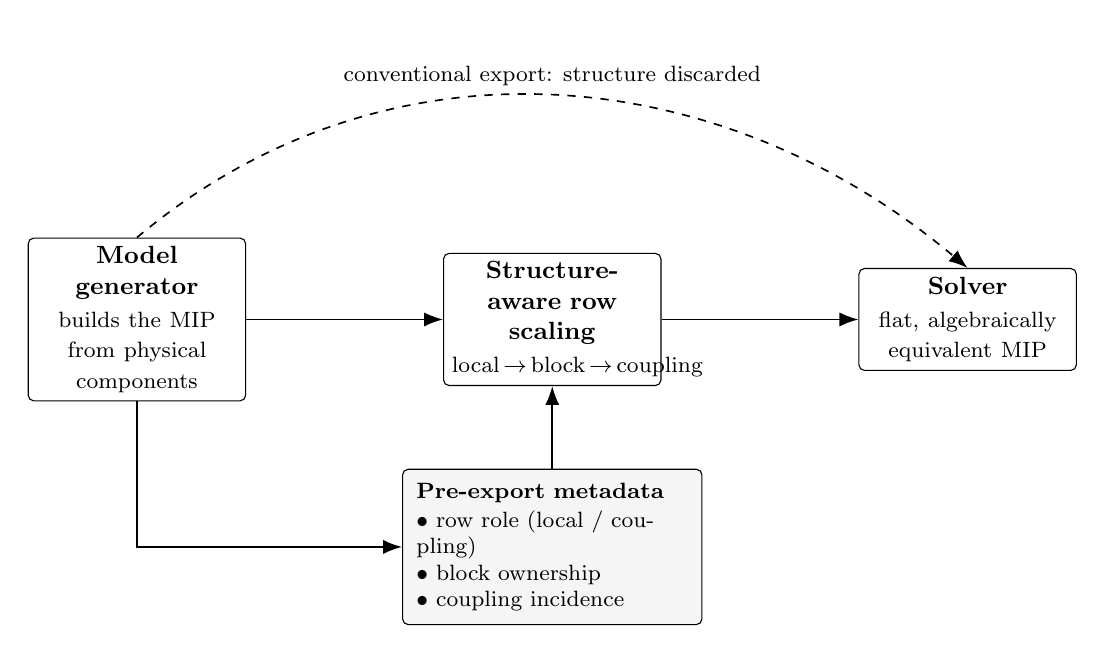
\begin{tikzpicture}[
  font=\small,
  >=Latex,
  box/.style={draw, rounded corners=2pt, align=center, minimum height=1.05cm,
              text width=2.55cm, inner sep=3pt},
  metabox/.style={draw, fill=black!4, rounded corners=2pt, align=left,
                  text width=3.45cm, inner sep=5pt, font=\footnotesize},
  arr/.style={-{Latex[length=2.4mm]}, semithick},
  darr/.style={-{Latex[length=2.4mm]}, semithick, dashed}
]
  \node[box] (gen) {\textbf{Model generator}\\[1pt]\footnotesize builds the MIP from
                    physical components};
  \node[box, right=2.5cm of gen] (scale) {\textbf{Structure-aware row scaling}\\[1pt]
                    \footnotesize local\,$\to$\,block\,$\to$\,coupling};
  \node[box, right=2.5cm of scale] (solver) {\textbf{Solver}\\[1pt]\footnotesize flat,
                    algebraically equivalent MIP};
  \node[metabox, below=1.05cm of scale] (meta) {\textbf{Pre-export metadata}\\[1pt]
                    $\bullet$ row role (local / coupling)\\
                    $\bullet$ block ownership\\
                    $\bullet$ coupling incidence};
  % main pipeline
  \draw[arr] (gen) -- (scale);
  \draw[arr] (scale) -- (solver);
  % the generator emits metadata, which keys the scaling
  \draw[arr] (gen.south) |- (meta.west);
  \draw[arr] (meta.north) -- (scale.south);
  % what a flat export throws away
  \draw[darr] (gen.north) to[out=40,in=140]
        node[above, font=\footnotesize] {conventional export: structure discarded}
        (solver.north);
\end{tikzpicture}
\caption{\DIFaddFL{The proposed layer in one picture. A generator assembles the MIP from physical
components and, in doing so, knows each row's role (local or coupling), which block owns
each variable, and how coupling rows link blocks. A conventional export (dashed) hands the
solver a flat matrix in which this structure is lost. The structure-aware layer instead
reuses that pre-export metadata to choose positive row factors in a local--block--coupling
order, then exports an \emph{algebraically equivalent} MIP whose representation is better
scaled. The solver still receives a single flat matrix; only its numbers change.}}
\label{fig:overview}
\end{figure}

\DIFadd{The }\DIFaddend numerical rationale is also local--block--coupling. In an ideal block-diagonal matrix,
scalar block scaling can reduce scale separation between blocks \DIFdelbegin \DIFdel{, but it cannot repair the
intrinsic conditioning of a block. Once }\DIFdelend \DIFaddbegin \DIFadd{but cannot repair a block's
intrinsic conditioning; once }\DIFaddend coupling rows are added, their relevant magnitude is \DIFdelbegin \DIFdel{not just their raw coefficient size; it is }\DIFdelend their size
relative to the scaled local blocks\DIFaddbegin \DIFadd{, not their raw coefficients}\DIFaddend . Idealized conditioning
results make this \DIFdelbegin \DIFdel{distinction precise . They justify the architecture of the preprocessing rule, but they do not claim }\DIFdelend \DIFaddbegin \DIFadd{precise and justify the rule's architecture, without claiming }\DIFaddend to predict
mixed-integer runtime.

We test the method on short-term hydrothermal dispatch\DIFdelbegin \DIFdel{. The methodological contribution is not a new hydrothermal formulation ; rather, the dispatch platform is }\DIFdelend \DIFaddbegin \DIFadd{, used not as a new formulation but as }\DIFaddend a
demanding testbed\DIFdelbegin \DIFdel{for the preprocessing idea. It naturally }\DIFdelend \DIFaddbegin \DIFadd{: it }\DIFaddend creates local hydro, thermal, market, shortage, and demand modules \DIFdelbegin \DIFdel{, then links them through global balance equations. The coefficients mix }\DIFdelend \DIFaddbegin \DIFadd{linked
by global balances, with coefficients mixing }\DIFaddend water volumes, turbine flows, power outputs, \DIFdelbegin \DIFdel{generation costs,
shortage penalties, and demand balances. The testbed therefore combines engineering structure with numerical }\DIFdelend \DIFaddbegin \DIFadd{costs,
and penalties---block structure with strong }\DIFaddend scale heterogeneity. \DIFaddbegin \DIFadd{The intended generality,
however, is the generated block-structured MIP, not the hydrothermal equations. The layer
requires only metadata that many modular generators already have---which rows are local, which
block owns a variable or constraint, which global rows couple blocks---while reservoir dynamics,
turbine curves, and market costs determine the instances but never enter the scaling rule. The
hydrothermal model thus supplies a realistic stress test for a layer that targets any generated
MIP with local components and sparse global coupling.
}\DIFaddend 

The hydrothermal formulation used in the experiments descends from models for the
R\'io Negro hydroelectric complex \DIFdelbegin \DIFdel{, extensions to }\DIFdelend \DIFaddbegin \DIFadd{and extensions to hydrothermal dispatch with }\DIFaddend Salto
Grande, \DIFdelbegin \DIFdel{and enriched hydrothermal
variants }\DIFdelend developed by Risso and coauthors, together with a modular C++ implementation
used as the experimental platform
\DIFdelbegin \DIFdel{\citep{risso2025rioNegro,risso2025uruguayRiver,risso2026enriched,rodriguez2025thesis}}\DIFdelend \DIFaddbegin \DIFadd{\cite{risso2025rioNegro,risso2025uruguayRiver,rodriguez2025thesis}}\DIFaddend .
We take the formulation as given and insert the proposed preprocessing layer after model
generation and before solver invocation.

The paper makes three claims of different strength\DIFdelbegin \DIFdel{. The }\DIFdelend \DIFaddbegin \DIFadd{: the }\DIFaddend algebraic claim is exact \DIFdelbegin \DIFdel{: }\DIFdelend \DIFaddbegin \DIFadd{(}\DIFaddend positive row
scaling preserves the MIP\DIFdelbegin \DIFdel{. The }\DIFdelend \DIFaddbegin \DIFadd{); the }\DIFaddend numerical claim is empirical \DIFdelbegin \DIFdel{: in the tested hydrothermal instances, generator-aware }\DIFdelend \DIFaddbegin \DIFadd{(structure-aware }\DIFaddend scaling improves
solver-facing conditioning \DIFdelbegin \DIFdel{measures. The }\DIFdelend \DIFaddbegin \DIFadd{in the tested instances); and the }\DIFaddend performance claim is conditional
\DIFdelbegin \DIFdel{: under Gurobi , }\DIFdelend \DIFaddbegin \DIFadd{(under Gurobi }\DIFaddend the improved representation often reduces robust runtime or deterministic effort\DIFdelbegin \DIFdel{; }\DIFdelend \DIFaddbegin \DIFadd{,
while }\DIFaddend under CPLEX 22.1.2.0 \DIFdelbegin \DIFdel{, the same external transformations do notproduce a robust runtime gain. Thus the }\DIFdelend \DIFaddbegin \DIFadd{it does not). The }\DIFaddend method improves representation\DIFdelbegin \DIFdel{, while }\DIFdelend \DIFaddbegin \DIFadd{; }\DIFaddend acceleration depends
on how the solver uses \DIFdelbegin \DIFdel{that representation}\DIFdelend \DIFaddbegin \DIFadd{it}\DIFaddend .

The rest of the paper follows this chain of evidence. \Cref{sec:related-work} identifies
the research niche. \Cref{sec:model} defines the generated model structure and testbed.
\Cref{sec:scaling} gives the scaling method. \Cref{sec:experimental-design} explains how
the experiments test the claims. \Cref{sec:results} reports numerical and runtime
evidence. \Cref{sec:discussion} interprets that evidence and answers likely objections.
\Cref{sec:validity} states the main limitations and reproducibility implications, and
\cref{sec:conclusion} summarizes the contribution.

\section{Related work}
\label{sec:related-work}
% -------------------------------------------------------------------------

The literature \DIFdelbegin \DIFdel{establishes the setting for the paper }\DIFdelend \DIFaddbegin \DIFadd{sets the stage }\DIFaddend but leaves a specific niche. \DIFdelbegin \DIFdel{The hydrothermal-dispatch literature supplies realistic generated engineering models . Numerical-scaling literature supplies flat-matrix preprocessing tools. Work on generated formulations explains why model-generation information may remain available before export. The missing argument is not that scaling can be useful in general; that is already well known}\DIFdelend \DIFaddbegin \DIFadd{Hydrothermal-dispatch models provide realistic generated block-structured MIPs with heterogeneous units and global balances; numerical-scaling work explains why coefficient magnitudes matter, but its standard tools operate on the exported matrix; and formulation-quality practice shows that algebraic representation can matter as much as the underlying set}\DIFaddend . The missing argument is narrower \DIFdelbegin \DIFdel{: when the generator knows the block and coupling role of each row, that information can guide algebraically equivalent row scalings}\DIFdelend \DIFaddbegin \DIFadd{than ``scaling is useful'': when a generator still knows each row's role and each variable's block, that metadata can be used as numerical information before export}\DIFaddend , and the \DIFdelbegin \DIFdel{value of those scalings must be judged through both numerical evidence and solver behavior}\DIFdelend \DIFaddbegin \DIFadd{resulting transformation must be evaluated separately as an algebraic equivalence, a representation change, and a solver-dependent performance intervention}\DIFaddend .

\subsection{Hydrothermal dispatch and MIP formulations}

Hydrothermal dispatch has been studied with dynamic programming, stochastic dual
dynamic programming, nonlinear programming, and mathematical programming. Classical
references emphasize the trade-off between thermal generation costs, hydro opportunity
costs, demand satisfaction, and intertemporal reservoir management
\DIFdelbegin \DIFdel{\citep{wood2013power,conejo2010decision}}\DIFdelend \DIFaddbegin \DIFadd{\cite{wood2013power,conejo2010decision}}\DIFaddend . In short-term settings, MIP formulations are
attractive because they incorporate discrete decisions, piecewise-linear approximations,
local operating constraints, and system-wide balance equations in a single model
\DIFdelbegin \DIFdel{\citep{vielma2015formulation}}\DIFdelend \DIFaddbegin \DIFadd{\cite{vielma2015formulation}}\DIFaddend .

This literature motivates the \DIFdelbegin \DIFdel{testbed but does not define the paper's methodological contribution. The objective here is not to redesign the hydrothermal model itself. Instead, the dispatch model acts as }\DIFdelend \DIFaddbegin \DIFadd{experimental domain but not the novelty claim. The dispatch model is used because it is }\DIFaddend a representative generated \DIFdelbegin \DIFdel{engineering MIPwith }\DIFdelend \DIFaddbegin \DIFadd{block-structured MIP: }\DIFaddend local physical modules \DIFdelbegin \DIFdel{and global coupling equations}\DIFdelend \DIFaddbegin \DIFadd{are created separately, their variables have heterogeneous units, and a smaller set of global rows links the modules through system-wide balances. These are precisely the structural features exploited by the preprocessing layer}\DIFaddend .

\subsection{Dispatch models used in this study}

The computational experiments use a reference formulation from a research line on
MIP-based dispatch models for the Uruguayan power system. Risso et al. introduced a mixed combinatorial optimization model for the
R\'io Negro hydroelectric complex \DIFdelbegin \DIFdel{\citep{risso2025rioNegro}, }\DIFdelend \DIFaddbegin \DIFadd{\cite{risso2025rioNegro} and }\DIFaddend extended the
modeling line to \DIFdelbegin \DIFdel{the hydrothermal dispatch of
}\DIFdelend \DIFaddbegin \DIFadd{hydrothermal dispatch for }\DIFaddend the Uruguay River hydroelectric plant\DIFdelbegin \DIFdel{\citep{risso2025uruguayRiver},
and developed an
enriched formulation for the R\'io Negro complex with additional operational components
\citep{risso2026enriched}}\DIFdelend \DIFaddbegin \DIFadd{,
with emphasis on Salto Grande and coupled hydrothermal operation
\cite{risso2025uruguayRiver}}\DIFaddend . The implementation used here builds on a modular
C++ version of the R\'io Negro dispatch model \DIFdelbegin \DIFdel{\citep{rodriguez2025thesis}}\DIFdelend \DIFaddbegin \DIFadd{\cite{rodriguez2025thesis}}\DIFaddend .

This provenance fixes the scope of the experiments. The dispatch formulation, data
pipeline, and physical components are \DIFdelbegin \DIFdel{not redesigned}\DIFdelend \DIFaddbegin \DIFadd{taken as given}\DIFaddend . The proposed method acts after the
model has been generated and before the solver is called. \DIFaddbegin \DIFadd{Consequently, any observed
difference between variants is attributed to an algebraically equivalent representation of
the same generated MIP, not to a modified dispatch model.
}\DIFaddend 

\subsection{Numerical scaling \DIFdelbegin \DIFdel{in mathematical programming}\DIFdelend \DIFaddbegin \DIFadd{and solver-facing representation}\DIFaddend }

Scaling is a standard preprocessing operation in linear and mixed-integer optimization.
Multiplying a constraint by a positive factor preserves the feasible region but changes
the numerical magnitudes passed to the solver. These magnitudes can affect feasibility
tolerances, relaxation stability, presolve transformations, \DIFaddbegin \DIFadd{cut generation, basis quality,
}\DIFaddend and the numerical behavior of LP relaxations. Practical guidelines for difficult LP and
MIP models warn that large coefficient ranges and poor scaling can harm solver
performance even when the mathematical formulation is correct \DIFdelbegin \DIFdel{\citep{klotz2013lp,klotz2013mip}}\DIFdelend \DIFaddbegin \DIFadd{\cite{klotz2013lp,klotz2013mip}}\DIFaddend .

\DIFaddbegin \DIFadd{This paper uses that observation in a restricted way: it does not claim coefficient compression
is itself an objective, nor that a smaller coefficient range must speed up branch-and-bound. A MIP
solver is a pipeline---presolve, internal scaling, root relaxation, cuts, heuristics, incumbents,
branching, node processing, termination---whose stages can respond differently to the same
external scaling. The experiments therefore distinguish exported coefficient-range ratios from
solver-level conditioning diagnostics and from runtime, a distinction central to interpreting the
Gurobi--CPLEX contrast.
}

\subsection{\DIFadd{Generic equilibration and its limitation for generated models}}

\DIFaddend Generic equilibration procedures balance rows and columns according to matrix norms.
\DIFaddbegin \DIFadd{This is a mature subfield of numerical linear algebra. Geometric-mean and
arithmetic-mean ($\ell_\infty$) scaling normalize each row or column by an average of its
coefficient magnitudes \cite{tomlin1975scaling}; Curtis--Reid scaling chooses logarithmic
diagonal factors that minimize a least-squares measure of coefficient spread
\cite{curtisreid1972}; Sinkhorn--Knopp iteration drives a nonnegative matrix toward a
doubly stochastic form by alternating row and column normalization \cite{sinkhorn1967};
and }\DIFaddend Ruiz-type \DIFdelbegin \DIFdel{scaling is a representative method: it }\DIFdelend \DIFaddbegin \DIFadd{scaling }\DIFaddend iteratively equilibrates row and column norms through diagonal
transformations \DIFdelbegin \DIFdel{\citep{ruiz2001scaling}}\DIFdelend \DIFaddbegin \DIFadd{\cite{ruiz2001scaling}. These methods are the standard tools and are
already embedded in solver presolve and internal scaling \cite{achterberg2020presolve}.
Their computational payoff, however, is known to be irregular: the largest empirical study
of LP scaling to date found that no scaling method consistently improves---and can even
degrade---simplex performance across solvers \cite{elble2012scaling}, an early warning that
coefficient compression alone is not the lever}\DIFaddend .
Such methods are useful because they are model-agnostic \DIFaddbegin \DIFadd{and can be applied after export}\DIFaddend .
That strength is also their limitation \DIFdelbegin \DIFdel{here. They balance
the exported matrix but do not necessarily know }\DIFdelend \DIFaddbegin \DIFadd{in the setting considered here. A flat-matrix method
can see coefficient magnitudes and sparsity, but it is not told }\DIFaddend whether a row \DIFdelbegin \DIFdel{represents a local
device
restrictionor a global coupling equation}\DIFdelend \DIFaddbegin \DIFadd{is a local
turbine restriction, a thermal bound, a market-cost relation, a shortage constraint, or a
system-wide balance}\DIFaddend .

\DIFdelbegin \subsection{\DIFdel{Generated formulations and the remaining niche}}
%DIFAUXCMD
\addtocounter{subsection}{-1}%DIFAUXCMD
\DIFdelend \DIFaddbegin \DIFadd{Against this background, the proposed rule is not a new equilibration kernel: its local row
factor is, in isolation, a geometric mean of the per-row coefficient extremes, as in
geometric-mean scaling. What is new is \emph{where the scales come from and in what order}---the
factors are keyed to generator metadata (row role, block ownership, coupling incidence) rather
than the flat matrix, and applied in a local--block--coupling order so coupling rows are
normalized relative to the already-scaled blocks they connect, not their raw coefficients. A flat
method (Ruiz, Curtis--Reid, geometric-mean, Sinkhorn--Knopp) cannot make this
local-versus-coupling distinction, because role information is exactly what export discards. Concretely, take two rows with
identical coefficients: a flat method sees one row and scales them alike, whereas the
structure-aware rule need not. If one is a local block row and the other a coupling row, the
local row is scaled by its own coefficients while the coupling row is scaled relative to the
\emph{already-scaled} blocks it links---so a coupling row with small raw coefficients can still
receive a large factor when it joins a poorly-scaled block, and conversely. Identical numbers,
different roles, different factors: that is the lever a flat matrix cannot expose. The
model stays monolithic, as with generic scaling: an external, auditable layer that uses
generator metadata before the exported matrix loses it.
}\DIFaddend 

\DIFdelbegin \DIFdel{A modular model generator provides information that is not explicit in the coefficient
matrix alone. Each module contributes local rows and variables, while global rows couple
several modules. Treating all rows identically can ignore this modeling structure. Generator-aware preprocessing exploits this distinction while leaving the feasible region
unchanged. }\DIFdelend \DIFaddbegin \subsection{\DIFadd{Formulation quality, generated structure, and decomposition}}
\DIFaddend 

The \DIFdelbegin \DIFdel{present work occupies the niche between generic scaling and }\DIFdelend \DIFaddbegin \DIFadd{MIP literature also stresses that formulation quality matters: two algebraically
related formulations can describe the same modeling intention but lead to different
relaxations, numerics, and search behavior \cite{vielma2015formulation}. The present
work is adjacent to that tradition but changes a different object. It does not strengthen
the formulation, add valid inequalities, alter variables, or change the feasible set. It
changes only the positive row multipliers applied to complete constraints.
}

\DIFadd{The method is also adjacent to }\DIFaddend structural decomposition. Like \DIFdelbegin \DIFdel{decomposition, it uses block structure; unlike }\DIFdelend Dantzig--Wolfe, Benders, or
Lagrangian \DIFaddbegin \DIFadd{approaches, it recognizes local blocks and global linking rows. Unlike those
}\DIFaddend methods, it does not decompose the optimization problem\DIFaddbegin \DIFadd{, introduce a master problem, or
exchange prices or cuts between subproblems}\DIFaddend . The solver still receives one monolithic MIP.
The \DIFdelbegin \DIFdel{only change is an algebraically equivalent row scaling
chosen from generator-level information. For benchmarking, we use performance profiles,
a standard tool for comparing optimization algorithms over heterogeneous instance sets
\citep{dolan2002performance}}\DIFdelend \DIFaddbegin \DIFadd{use of block structure is numerical rather than algorithmic decomposition: block
metadata guide the representation presented to the solver}\DIFaddend .

\DIFaddbegin \subsection{\DIFadd{Remaining niche}}

\DIFaddend The resulting contribution is deliberately narrow: it tests whether local rows, block scales, and
coupling rows should be treated as different numerical objects before a generated \DIFdelbegin \DIFdel{engineering }\DIFdelend \DIFaddbegin \DIFadd{block-structured }\DIFaddend MIP
is exported\DIFdelbegin \DIFdel{to a commercial solver}\DIFdelend \DIFaddbegin \DIFadd{. The performance comparison rests on distributional evidence over heterogeneous
instances rather than a single runtime average, using performance profiles
\cite{dolan2002performance}, paired tests, deterministic-effort metrics, and solver-level
conditioning diagnostics}\DIFaddend .

\section{Materials and methods: generated modular formulation and testbed}
\label{sec:model}
% -------------------------------------------------------------------------

We now define the objects that the scaling rule changes and the objects it must leave
unchanged. The generator supplies the block structure; the preprocessing layer changes the
row magnitudes; the solver then receives an algebraically equivalent MIP. The dispatch
model itself is not new. What matters here is the structure that the generator exposes and
the original scale in which all feasibility and objective checks are evaluated after the
solve. We consider generated modular MIP instances formulated as
\begin{equation}
\begin{aligned}
  \min_{x} \quad & c^\top x \\
  \text{s.t.} \quad & Ax \le b, \\
  & x_j \in \Z, \qquad j \in \mathcal{I}, \\
  & x_j \in \R, \qquad j \notin \mathcal{I}.
\end{aligned}
\label{eq:generic-mip}
\end{equation}
In the general generated setting, the vector $x$ collects all variables created by the
modules, while $A$ and $b$ contain both local component constraints and global linking
constraints. In the hydrothermal testbed used here, $x$ includes generation, reservoir,
flow, spillage, shortage, and operating variables. Equalities are represented either
explicitly or by pairs of inequalities, depending on the solver interface.

\DIFaddbegin \DIFadd{The notation is intentionally application-agnostic: the layer uses the generator's structural
map---row role, block ownership, coupling incidence---not hydrological, thermal, or economic
semantics. The hydrothermal variables above explain the physical origin of the coefficients;
they are not assumptions of the scaling method.
}

\DIFaddend \subsection{Hydrothermal dispatch testbed and scope}

The computational testbed uses the reference model generated by the modular dispatch
platform developed around R\'io Negro and Salto Grande hydrothermal dispatch models
\DIFdelbegin \DIFdel{\citep{risso2025rioNegro,risso2025uruguayRiver,risso2026enriched,rodriguez2025thesis}}\DIFdelend \DIFaddbegin \DIFadd{\cite{risso2025rioNegro,risso2025uruguayRiver,rodriguez2025thesis}}\DIFaddend .
The application is useful because it exhibits the target structure: local modules
with heterogeneous physical units and global rows that couple those modules through
system-wide balances. The hydraulic, thermal, and market-cost constraints are those of
the reference model and its implementation.

\DIFdelbegin \DIFdel{The paper therefore separates the preprocessing idea from the application that tests it . The proposed }\DIFdelend \DIFaddbegin \DIFadd{A caveat about those heterogeneous units is in order, because it is tempting to read the
imbalance as artificial. The unit heterogeneity (reservoir volumes in $\mathrm{hm}^3$, flows in
$\mathrm{m}^3/\mathrm{s}$, power in MW) lives on the \emph{variables}---the columns---and
rescaling units is, mathematically, column scaling. Two points keep this from being a hidden
lever. First, column scaling of a continuous variable is an exact reformulation: it leaves the
optimum unchanged and can only affect \emph{runtime}, never the solution. Moreover it cannot be
applied to integer variables at all---$x\in\mathbb{Z}$ with $x=s\,x'$ makes $x'$ non-integer---so
in a MIP unit normalization is necessarily partial (continuous columns only) and need not leave the
matrix better balanced relative to the integer columns. Second, our column-normalizing baseline
(\methodRuizCols{}), which equilibrates the continuous columns toward unit $\infty$-norm, is the
weakest variant in runtime, and degrades further as that normalization is pushed harder---in line
with aggressive scaling hurting rather than helping the MIP search (\cref{subsec:internal-scaling}).
The lever that moves runtime in this testbed is therefore on the rows, not the columns. We do not
claim that a clean, one-shot change of units would harm the model---that is a separate question;
the narrower point is that the runtime gain comes from structural row scaling, not from attacking
the units. And the base is not an artificially ill-scaled straw man: it already runs under the
solver's own internal equilibration, and no internal scaling setting matches the structure-aware
variants (\cref{subsec:internal-scaling}).
}

\DIFadd{The }\DIFaddend method acts on the generated algebraic model\DIFdelbegin \DIFdel{; it does not modify }\DIFdelend \DIFaddbegin \DIFadd{, not }\DIFaddend the physical dispatch formulation\DIFdelbegin \DIFdel{. All preprocessing transformations }\DIFdelend \DIFaddbegin \DIFadd{: every transformation }\DIFaddend must preserve the feasible set and \DIFdelbegin \DIFdel{must allow }\DIFdelend \DIFaddbegin \DIFadd{let }\DIFaddend objective values, constraint violations, and operational variables \DIFdelbegin \DIFdel{to be interpreted }\DIFdelend \DIFaddbegin \DIFadd{be read }\DIFaddend in the original scale after solution. \DIFaddbegin \DIFadd{It never uses a hydro-specific rule (reservoir priority, turbine efficiency, unit commitment) to choose factors---those details generate the rows, and only their structural role in the block-coupled MIP is used afterward.
}\DIFaddend 

\subsection{Block structure}

The method targets models generated by components or agents. Each component
$i\in\mathcal{B}$ creates local variables $x_i$, contributes local constraints
$A_i x_i\le b_i$, and appears in a smaller number of global constraints. \DIFaddbegin \DIFadd{Let
$\mathcal{R}_i$ denote the local row index set of component $i$. }\DIFaddend In the hydrothermal
testbed, these components include hydro, thermal, market, and demand modules. If $u_{\mathrm{loc}}$ stacks all local variables and $g$ denotes an aggregate
coupling variable, the row structure can be written schematically as
\begin{equation}
\begin{bmatrix}
D & 0 \\
0 & I_T \\
L & -I_T
\end{bmatrix}
\begin{bmatrix}
u_{\mathrm{loc}} \\
g
\end{bmatrix}
\sim
\begin{bmatrix}
b \\
d \\
0
\end{bmatrix},
\qquad
D=\diag(A_1,\ldots,A_B).
\label{eq:compact-dispatch-structure}
\end{equation}
The first block contains local component restrictions. The second block represents an
aggregate system restriction. The third block contains coupling equations that link local
component decisions with the aggregate system variable. In the dispatch application,
these rows correspond to demand and balance relationships. Equivalently, after row and
column permutations, the coefficient matrix has the block form
\begin{equation}
A =
\begin{bmatrix}
A_1 & 0   & \cdots & 0 \\
0   & A_2 & \cdots & 0 \\
\vdots & \vdots & \ddots & \vdots \\
0   & 0   & \cdots & A_B \\
L_1 & L_2 & \cdots & L_B
\end{bmatrix},
\qquad
b =
\begin{bmatrix}
b_1\\ b_2\\ \vdots\\ b_B\\ h
\end{bmatrix}.
\label{eq:block-matrix}
\end{equation}
The matrices $A_i$ encode local restrictions. The matrices $L_i$ encode each block's contribution to the global coupling rows, such as demand balance in the hydrothermal
testbed.

This structure suggests three scaling decisions: scale local rows inside each block; compute representative block scales after local row scaling; and scale global coupling rows with those block scales. The goal is to reduce harmful scale heterogeneity without erasing the modular meaning of the formulation.

\subsection{Algebraic equivalence and spectral diagnostics}
\label{subsec:equivalence-diagnostics}

We restrict the preprocessing layer to positive row scalings. This restriction makes the
transformation auditable: variables keep their original units, and the generated MIP remains
the same optimization problem. Let $D_r=\diag(d_1,\ldots,d_m)$, with $d_r>0$ for every
row. We replace $(A,b)$ by
\begin{equation}
\widetilde A = D_r A,
\qquad
\widetilde b = D_r b .
\label{eq:row-scaling}
\end{equation}
For every vector $x$,
\begin{equation}
Ax\le b
\quad\Longleftrightarrow\quad
D_rAx\le D_rb,
\label{eq:row-scaling-equivalence}
\end{equation}
because each component of the inequality is multiplied by a strictly positive scalar.
Thus positive row scaling preserves the feasible set, the integer restrictions, and the
objective function. Any difference observed after preprocessing must therefore come from
the numerical representation seen by the solver, not from a different mathematical MIP.

The theoretical arguments below use the spectral condition number as a diagnostic of linear-algebraic sensitivity. For a real matrix $M$, define
\begin{equation}
\kappa_2(M)=
\frac{\sigma_{\max}(M)}{\sigma_{\min}^{+}(M)},
\label{eq:spectral-condition}
\end{equation}
where $\sigma_{\max}(M)$ is the largest singular value and $\sigma_{\min}^{+}(M)$ is the
smallest positive singular value. For rectangular matrices, this ratio is used only as a
diagnostic over the nonzero singular spectrum; in square nonsingular benchmarks, rank
deficiency is interpreted as infinite condition number. This diagnostic does not characterize the full difficulty of a MIP. A MIP solver also depends on presolve, cuts, branching, primal heuristics, incumbent discovery, feasibility tolerances, and integrality. The role of $\kappa_2$ is narrower: it provides an idealized matrix argument explaining why local rows and coupling rows should not be scaled in exactly the same way.

\subsection{Ideal block scaling}
\label{subsec:ideal-block-scaling}

The block structure is not only a modeling convenience. It identifies what scalar scaling
can and cannot repair. In a purely block-diagonal matrix $D=\diag(A_1,\ldots,A_B)$, a
single scalar per block can remove differences of scale between blocks, but it cannot
improve the intrinsic conditioning of an individual block. The following benchmark makes
this statement precise in the ideal square nonsingular case.

\begin{proposition}[Ideal scalar scaling of block-diagonal matrices]
\label{prop:ideal-block-scaling}
Let $D=\diag(A_1,\ldots,A_B)$, where every $A_i$ is square and nonsingular. Let
$M_i=\sigma_{\max}(A_i)$ and $m_i=\sigma_{\min}(A_i)>0$. Then
\begin{equation}
\min_{\alpha_i>0}
\kappa_2\!\left(\diag(\alpha_1 I,\ldots,\alpha_B I)D\right)
=
\max_i \kappa_2(A_i).
\label{eq:ideal-block-minimax}
\end{equation}
One minimizer is
\begin{equation}
\alpha_i=\frac{1}{\sqrt{M_i m_i}}
=
\frac{1}{\sqrt{\sigma_{\max}(A_i)\sigma_{\min}(A_i)}} .
\label{eq:ideal-block-factor}
\end{equation}
\end{proposition}

\begin{proof}
For fixed positive scalars $\alpha_i$, the scaled matrix is block diagonal:
\begin{equation*}
\diag(\alpha_1 I,\ldots,\alpha_B I)D
=
\diag(\alpha_1 A_1,\ldots,\alpha_B A_B).
\end{equation*}
The singular values of a block-diagonal matrix are the union of the singular values of
its blocks. Therefore, for every $i$,
\begin{equation*}
\kappa_2\!\left(\diag(\alpha_1 A_1,\ldots,\alpha_B A_B)\right)
\ge
\kappa_2(\alpha_i A_i)
=
\kappa_2(A_i).
\end{equation*}
Taking the maximum over $i$ gives the lower bound
\begin{equation*}
\kappa_2\!\left(\diag(\alpha_1 A_1,\ldots,\alpha_B A_B)\right)
\ge
\max_i \kappa_2(A_i)
\end{equation*}
for every admissible block scaling.

Now choose $\alpha_i=(M_i m_i)^{-1/2}$. Then the largest and smallest singular values of
$\alpha_i A_i$ are
\begin{align*}
\sigma_{\max}(\alpha_i A_i)
&=\sqrt{\frac{M_i}{m_i}}=\sqrt{\kappa_2(A_i)},\\
\sigma_{\min}(\alpha_i A_i)
&=\sqrt{\frac{m_i}{M_i}}=\frac{1}{\sqrt{\kappa_2(A_i)}}.
\end{align*}
Because the singular values of the complete block-diagonal matrix are obtained by
pooling the singular values of its blocks,
\begin{equation*}
\sigma_{\max}\!\left(\diag(\alpha_1 A_1,\ldots,\alpha_B A_B)\right)
=
\sqrt{\max_i \kappa_2(A_i)},
\end{equation*}
and
\begin{equation*}
\sigma_{\min}\!\left(\diag(\alpha_1 A_1,\ldots,\alpha_B A_B)\right)
=
\frac{1}{\sqrt{\max_i \kappa_2(A_i)}}.
\end{equation*}
The resulting condition number is $\max_i\kappa_2(A_i)$, matching the lower bound.
\end{proof}

This proposition is not used as an algorithmic recipe. The generated MIPs considered in
this paper contain rectangular local matrices, inequalities, bounds, redundant rows, and
integer variables; computing singular-value-based block scalings would not be a practical
external preprocessing rule for the exported MIP. The proposition instead justifies the
architecture of the method. First, poor scale separation between blocks should be treated
differently from poor conditioning inside a block. Second, after local row scaling, each
block should contribute a representative scale before global coupling rows are processed.
The implemented rules therefore replace the ideal singular-value quantities
$(M_i,m_i)$ with coefficient-based proxies that are cheap to compute from the generated
model. These propositions are design principles, not performance theorems. They should not be read as predictive guarantees for the implemented
MIP preprocessing rule; they motivate the distinction between local rows, block scales,
and coupling rows.

\subsection{Effect of global coupling rows}
\label{subsec:global-coupling-theory}

Local block scaling does not exhaust the numerical issue because the generated model is
not purely block diagonal. In the hydrothermal dispatch testbed, global rows couple local
agent decisions through demand and balance equations. The relevant schematic block is
\begin{equation}
A_B=
\begin{bmatrix}
D & 0\\
L & -I_T
\end{bmatrix},
\label{eq:balance-block-matrix}
\end{equation}
where $D=\diag(A_1,\ldots,A_B)$ represents the local blocks and $L$ collects the
coefficients by which local decisions enter the global balance. If $D$ is nonsingular, then
\begin{equation}
A_B=
\begin{bmatrix}
I & 0\\
LD^{-1} & -I_T
\end{bmatrix}
\begin{bmatrix}
D & 0\\
0 & I_T
\end{bmatrix}.
\label{eq:balance-factorization}
\end{equation}
This factorization separates local scale from coupling scale. The matrix $L$ by itself is
not the relevant object: the coupling felt by the balance row after the local block scales
are taken into account is $LD^{-1}$. Thus a row with moderate entries in $L$ can still be
numerically influential if some local block contains weak directions.

The next result makes the dependence on the effective coupling norm explicit.

\begin{proposition}[Conditioning of a triangular coupling factor]
\label{prop:triangular-coupling}
Let $R\in\R^{m\times n}$ and define
\begin{equation}
T_R=
\begin{bmatrix}
I_n & 0\\
R & I_m
\end{bmatrix}.
\end{equation}
If $\rho=\norm{R}_2$, then
\begin{equation}
\kappa_2(T_R)=
\left(\frac{\sqrt{\rho^2+4}+\rho}{2}\right)^2 .
\label{eq:link-condition}
\end{equation}
\end{proposition}

\begin{proof}
Let $R=U\Sigma V^\top$ be a singular value decomposition of $R$, with $U$ and $V$
orthogonal. Orthogonal multiplication does not change singular values, and hence
$T_R$ has the same singular values as
\begin{equation*}
\begin{bmatrix}
V^\top & 0\\
0 & U^\top
\end{bmatrix}
\begin{bmatrix}
I_n & 0\\
R & I_m
\end{bmatrix}
\begin{bmatrix}
V & 0\\
0 & U
\end{bmatrix}
=
\begin{bmatrix}
I_n & 0\\
\Sigma & I_m
\end{bmatrix}.
\end{equation*}
For each singular value $\sigma$ of $R$, the nontrivial part reduces to the two-dimensional
block
\begin{equation*}
B_\sigma=
\begin{bmatrix}
1 & 0\\
\sigma & 1
\end{bmatrix}.
\end{equation*}
The squared singular values of $B_\sigma$ are the eigenvalues of
\begin{equation*}
B_\sigma^\top B_\sigma=
\begin{bmatrix}
1+\sigma^2 & \sigma\\
\sigma & 1
\end{bmatrix},
\end{equation*}
namely
\begin{equation*}
\lambda_{\pm}(\sigma)=
\frac{\sigma^2+2\pm \sigma\sqrt{\sigma^2+4}}{2}.
\end{equation*}
Their product is one, and $\lambda_+(\sigma)$ is increasing for $\sigma\ge0$. Additional
directions associated with zero singular values of $R$ contribute singular values equal to
one. Therefore the largest squared singular value of $T_R$ is $\lambda_+(\rho)$ and the
smallest squared singular value is $1/\lambda_+(\rho)$. Consequently,
\begin{align*}
\kappa_2(T_R)
&=\lambda_+(\rho)\\
&=\frac{\rho^2+2+\rho\sqrt{\rho^2+4}}{2}\\
&=\left(\frac{\sqrt{\rho^2+4}+\rho}{2}\right)^2 .
\end{align*}
\end{proof}

Applied to \eqref{eq:balance-factorization}, the proposition shows that the balance row
should not be treated as an ordinary local row. Its numerical effect depends on the
effective coupling proxy $\norm{LD^{-1}}_2$, not only on the raw magnitude of the
entries in $L$. Moreover, if a common positive factor $\gamma$ is applied to the coupling
row, the scaled block satisfies
\begin{equation}
\begin{bmatrix}
D & 0\\
\gamma L & -\gamma I_T
\end{bmatrix}
=
\begin{bmatrix}
I & 0\\
\gamma LD^{-1} & -I_T
\end{bmatrix}
\begin{bmatrix}
D & 0\\
0 & \gamma I_T
\end{bmatrix}.
\label{eq:scaled-balance-factorization}
\end{equation}
Thus $\gamma$ changes both the effective coupling term and the relative scale of the
aggregate variable in the balance equation. This is the trade-off behind the proposed
coupling-row factor: global rows should be scaled after local rows, using block-level
representative scales, rather than by an isolated row norm. In the implemented variants,
$D^{-1}$ and singular values are replaced by coefficient-based block proxies, yielding a
cheap operational approximation to the ideal coupling measure.


\DIFaddbegin \subsection{\DIFadd{From ideal diagnostics to implementable proxies}}
\label{subsec:ideal-to-proxies}

\DIFadd{The two propositions establish \emph{which} numerical distinctions a structure-aware
rule must preserve, and thereby justify the architecture. They imply three design
requirements: local scale imbalance should be reduced before global coupling rows are
diagnosed; blocks should be summarized only after their local rows are on a comparable
scale; and a coupling row should be scaled relative to the blocks it connects, not only
relative to its own raw coefficient norm. The implemented method realizes exactly these
distinctions through coefficient-based proxies: they are cheap to compute from the
generated model before export, auditable because they depend only on visible row and
block metadata, and they avoid expensive or unstable singular-value information from the
rectangular, redundant, inequality-based matrices that arise in generated MIPs. The row
factor based on the geometric mean of the smallest and largest nonzero magnitudes is a
robust coefficient-scale proxy that centers each eligible row without changing variables,
bounds, integrality, or the objective.
}

\DIFadd{The coupling rule implements the same logic. In \cref{prop:triangular-coupling}, the
relevant ideal object is the effective coupling magnitude after local scaling, a term of
the form $LD^{-1}$; since generated blocks are rectangular, possibly redundant, and not
inverted by the preprocessing layer, the block scale $s_i$ used below is a representative
coefficient scale for block $i$ computed after local row scaling, and the coupling proxy
divides each coupling coefficient by the representative scale of the block owning its
column. This is a cheap, auditable surrogate for asking whether the coupling row is large
relative to the local numerical scale of the blocks it links.
}

\DIFadd{We state the scope of this argument once and plainly: the propositions describe square,
nonsingular blocks under exact SVD scaling, the proxies act on rectangular,
inequality-based matrices, and we establish no bound relating the proxy scale to the
ideal spectral factor in \cref{prop:ideal-block-scaling}. The propositions therefore
motivate the design, and its empirical validity is verified directly in the controlled
synthetic suite of \cref{subsec:synthetic-benchmark}, where blocks are small, singular
values are cheap to compute, and conditioning is measurable by construction.
}

\DIFadd{This bridge also explains why the proposed method is row-based. Positive row scaling
preserves the original units and domains of all variables; integer and binary variables do
not require reinterpretation, and objective coefficients are left in their original
economic units. Column scaling can be useful as a generic numerical device, so a
Ruiz-plus-column baseline is included in the experiments. It is not part of the proposed
structure-aware layer because the central claim is that row-role and coupling metadata
alone already provide useful pre-export numerical information while keeping the
transformation algebraically transparent.
}


\DIFaddend % -------------------------------------------------------------------------
\section{Numerical scaling method}
\label{sec:scaling}
% -------------------------------------------------------------------------

The scaling method keeps the same structural roles visible throughout: local rows, blocks, and coupling rows. Local rows receive row factors first. Blocks then inherit representative scales from their scaled local rows. Coupling rows receive their factors last, using the blocks they connect. This order is the algorithmic expression of the numerical argument in \cref{subsec:ideal-block-scaling,subsec:global-coupling-theory} \DIFaddbegin \DIFadd{and of the proxy interpretation in \cref{subsec:ideal-to-proxies}}\DIFaddend .

This section defines the numerical transformations tested in the results. The base variant is the unscaled model generated by the platform. The two proposed variants use the same local--block--coupling architecture but differ in whether the right-hand side participates in the scale diagnosis. Ruiz-type variants provide generic flat-matrix baselines. This organization makes two contrasts explicit. The comparison between \methodAug{} and \methodMat{} isolates the role of right-hand-side information within the same architecture; the comparison with Ruiz-type baselines tests whether generator-level row roles add information beyond generic flat-matrix equilibration.

\subsection{Base formulation}

The \methodBase{} variant is passed to the solver without external scaling. Internal
solver presolve and internal scaling remain enabled unless stated otherwise. All
speedups, objective deviations, and equivalence checks are computed relative to this
variant on the same instance, solver, and gap setting.

\subsection{Augmented \DIFdelbegin \DIFdel{generator-aware }\DIFdelend \DIFaddbegin \DIFadd{structure-aware }\DIFaddend scaling}
\label{subsec:strategy-1}

The first proposed variant, denoted \methodAug{}, computes row factors from both
coefficient magnitudes and right-hand sides. The motivation is that a generated row may
have moderate coefficients but a right-hand side in a very different physical or economic
scale. Such a row can still lead to a poorly balanced numerical representation.

For each local row $r$, define
\begin{equation}
\mathcal{S}_r^{A,b}
=
\left\{
\abs{a_{rj}}: a_{rj}\neq 0
\right\}
\cup
\left\{
\abs{b_r}: b_r\neq 0
\right\}.
\label{eq:augmented-set}
\end{equation}
If $\mathcal{S}_r^{A,b}\neq\emptyset$, let
\begin{equation}
M_r^{A,b}=\max \mathcal{S}_r^{A,b},
\qquad
m_r^{A,b}=\min \mathcal{S}_r^{A,b}.
\label{eq:augmented-extremes}
\end{equation}
The local row factor is
\begin{equation}
\alpha_r^{A,b}=\frac{1}{\sqrt{M_r^{A,b}m_r^{A,b}}}.
\label{eq:alpha-augmented}
\end{equation}
The scaled row is
\begin{equation}
\alpha_r^{A,b}a_r^\top x\le \alpha_r^{A,b}b_r.
\end{equation}

The augmented rule is not only a row-by-row normalization. It is a three-stage
\DIFdelbegin \DIFdel{generator-aware }\DIFdelend \DIFaddbegin \DIFadd{structure-aware }\DIFaddend procedure that first rescales local rows, then summarizes the resulting
local block scales, and finally uses those block scales to treat coupling rows separately.
After local scaling, let $\widetilde a_{rj}=\alpha_r^{A,b}a_{rj}$ for local rows. For each
local block $i$, define
\DIFdelbegin %DIFDELCMD < \begin{equation}
%DIFDELCMD < M_i^{A,b}
%DIFDELCMD < =
%DIFDELCMD < \max_{r\in A_i,\,j:\,\widetilde a_{rj}\neq 0}
%DIFDELCMD < \abs{\widetilde a_{rj}},
%DIFDELCMD < \qquad
%DIFDELCMD < m_i^{A,b}
%DIFDELCMD < =
%DIFDELCMD < \min_{r\in A_i,\,j:\,\widetilde a_{rj}\neq 0}
%DIFDELCMD < \abs{\widetilde a_{rj}}.
%DIFDELCMD < \label{eq:augmented-block-extremes}
%DIFDELCMD < \end{equation}%%%
\DIFdelend \DIFaddbegin \begin{equation}
M_i^{A,b}
=
\max_{r\in\mathcal{R}_i,\,j:\,\widetilde a_{rj}\neq 0}
\abs{\widetilde a_{rj}},
\qquad
m_i^{A,b}
=
\min_{r\in\mathcal{R}_i,\,j:\,\widetilde a_{rj}\neq 0}
\abs{\widetilde a_{rj}}.
\label{eq:augmented-block-extremes}
\end{equation}\DIFaddend 
The representative scale of block $i$ is
\begin{equation}
s_i^{A,b}=\sqrt{M_i^{A,b}m_i^{A,b}}.
\label{eq:augmented-block-scale}
\end{equation}
For a coupling row $r$, let $b(j)$ denote the local block associated with column $j$.
The effective coupling proxy used by \methodAug{} is
\begin{equation}
\widehat\rho_r^{A,b}
=
\sqrt{
\sum_j
\left(
\frac{\abs{a_{rj}}}{s_{b(j)}^{A,b}}
\right)^2
}.
\label{eq:augmented-coupling-rho}
\end{equation}
If $\widehat\rho_r^{A,b}>0$, the coupling-row factor is
\begin{equation}
\gamma_r^{A,b}=\frac{1}{\widehat\rho_r^{A,b}}.
\label{eq:augmented-coupling-factor}
\end{equation}
All factors are then clipped by the safeguards described below. This sequence is the
main structural feature of the proposed method: local physical scales are used first,
block scales are estimated after local normalization, and global coupling rows are scaled
only after the blocks they connect have been put on comparable numerical footing.

\subsection{Matrix-only \DIFdelbegin \DIFdel{generator-aware }\DIFdelend \DIFaddbegin \DIFadd{structure-aware }\DIFaddend scaling}
\label{subsec:strategy-2}

The second proposed variant, denoted \methodMat{}, uses the same row--block--coupling
architecture but excludes $b$ from the diagnosis. The right-hand side is still multiplied
by the selected row factor to preserve equivalence, but it does not influence factor
selection.

For each local row $r$, define the nonzero coefficient extremes
\begin{equation}
M_r^{A}=\max_{j:\,a_{rj}\neq 0}\abs{a_{rj}},
\qquad
m_r^{A}=\min_{j:\,a_{rj}\neq 0}\abs{a_{rj}}.
\label{eq:matrix-row-extremes}
\end{equation}
If the row has at least one nonzero coefficient, the row factor is
\begin{equation}
\alpha_r^{A}=\frac{1}{\sqrt{M_r^{A}m_r^{A}}}.
\label{eq:matrix-row-factor}
\end{equation}
The scaled row is
\begin{equation}
\alpha_r^{A}a_r^\top x\le \alpha_r^{A}b_r.
\end{equation}
This factor centers the smallest and largest nonzero coefficient magnitudes of the row
around a common scale. Unlike Euclidean-norm scaling, it does not directly depend on
the number of nonzeros in the row.

Let $\widetilde a_{rj}=\alpha_r^A a_{rj}$ after local row scaling. For each local block
$i$, define
\DIFdelbegin %DIFDELCMD < \begin{equation}
%DIFDELCMD < M_i^{A}
%DIFDELCMD < =
%DIFDELCMD < \max_{r\in A_i,\,j:\,\widetilde a_{rj}\neq 0}
%DIFDELCMD < \abs{\widetilde a_{rj}},
%DIFDELCMD < \qquad
%DIFDELCMD < m_i^{A}
%DIFDELCMD < =
%DIFDELCMD < \min_{r\in A_i,\,j:\,\widetilde a_{rj}\neq 0}
%DIFDELCMD < \abs{\widetilde a_{rj}}.
%DIFDELCMD < \label{eq:matrix-block-extremes}
%DIFDELCMD < \end{equation}%%%
\DIFdelend \DIFaddbegin \begin{equation}
M_i^{A}
=
\max_{r\in\mathcal{R}_i,\,j:\,\widetilde a_{rj}\neq 0}
\abs{\widetilde a_{rj}},
\qquad
m_i^{A}
=
\min_{r\in\mathcal{R}_i,\,j:\,\widetilde a_{rj}\neq 0}
\abs{\widetilde a_{rj}}.
\label{eq:matrix-block-extremes}
\end{equation}\DIFaddend 
The representative block scale is
\begin{equation}
s_i^A=\sqrt{M_i^A m_i^A}.
\label{eq:matrix-block-scale}
\end{equation}
No additional multiplier is applied to all rows or columns of block $i$ at this stage.
The quantity $s_i^A$ is an auxiliary representative scale: it is used only to
normalize the contribution of block $i$ when the coupling-row proxy is computed.

For a coupling row $r$, let $b(j)$ denote the block associated with column $j$. Define
\begin{equation}
\widehat{\rho}_r^{A}
=
\sqrt{
\sum_j
\left(
\frac{\abs{a_{rj}}}{s_{b(j)}^{A}}
\right)^2
}.
\label{eq:matrix-coupling-rho}
\end{equation}
If $\widehat{\rho}_r^{A}>0$, the coupling-row factor is
\begin{equation}
\gamma_r^{A}=\frac{1}{\widehat{\rho}_r^{A}}.
\label{eq:matrix-coupling-factor}
\end{equation}

The comparison between \methodAug{} and \methodMat{} isolates the empirical value of
including the right-hand side in the scaling diagnosis. Both variants preserve the same
structural architecture; they differ only in whether $b$ participates in factor selection.

\subsection{Safeguards}

All applied scaling factors---the local row factors and the coupling-row factors in the
augmented or matrix-only variants---are subject to two per-factor safeguards, applied
independently to each factor. The representative block scales $s_i$ are auxiliary
quantities used to compute coupling-row proxies; they are not applied as independent
row or column scalings.

\paragraph{Near-identity threshold}
A factor is applied only if it departs from one by at least a factor of $u=2$; factors
falling in the band $[\,1/u,\;u\,]=[0.5,\,2]$ are treated as negligible and skipped:
\begin{equation}
\theta \text{ is applied}
\iff
\left(\theta \le \frac{1}{u}\right)\ \text{or}\ \left(\theta \ge u\right),
\qquad u=2 .
\label{eq:near-identity}
\end{equation}
This prevents re-scaling rows or coupling rows that are already at a reasonable scale.

\paragraph{Admissible coefficient range}
A factor is applied only if it keeps every affected coefficient within the window
$[\varepsilon_{\min},\varepsilon_{\max}] = [10^{-9},\,10^{9}]$. Writing
$c_{\min}$ and $c_{\max}$ for the smallest and largest magnitudes of the affected
coefficients, the factor $\theta$ is admitted only if
\begin{equation}
\begin{aligned}
\varepsilon_{\min} &\le c_{\min}\,\theta,
& c_{\max}\,\theta &\le \varepsilon_{\max},\\
[\varepsilon_{\min},\varepsilon_{\max}]&=[10^{-9},\,10^{9}].
\end{aligned}
\label{eq:coef-window}
\end{equation}
Otherwise, the factor is not applied and the corresponding row or coupling row is left at its base scale. The coupling factor is additionally hard-clipped to
$\gamma \in [10^{-8},\,10^{8}]$ prior to this check.

Because each admitted factor is a strictly positive multiplier applied to a complete
constraint---both its coefficients and its right-hand side---the feasible set and the
objective value are preserved exactly. The safeguards therefore restrict only the
numerical aggressiveness of the transformation, never its equivalence to the base model.


\subsection{Ruiz-type baselines}

We compare the proposed variants with two generic baselines. The first,
\methodRuiz{}, applies iterative row equilibration based on the maximum norm. The
second, \methodRuizCols{}, combines Ruiz-type row equilibration with continuous-column
scaling and physical normalization. These baselines separate the effect of generic
coefficient compression from the effect of exploiting model structure.

\DIFaddbegin \DIFadd{\methodRuiz{} is deliberately not a weak foil. Max-norm Ruiz equilibration is a standard,
well-regarded scheme from the same family of row/column equilibrators embedded in commercial
presolve, so it represents what a strong flat-matrix routine---one that sees coefficient
magnitudes but not row roles---can achieve, and \methodRuizCols{} additionally grants it the
column-scaling lever the structure-aware rule forgoes. The comparison is therefore conservative
by design, and it is \emph{not} a contest against the solver's internal numerical engineering:
internal scaling and presolve stay enabled in every run, and the dedicated control for ``could
the solver have done this itself'' is the internal-scaling baseline of
\cref{subsec:internal-scaling}, not the Ruiz contrast. The question the baselines isolate is
narrower---whether generator-level row roles and coupling incidence carry numerical information
that a flat-matrix equilibrator, however well tuned, cannot recover once export has discarded
those roles. Every variant hands the solver the same monolithic MIP and lets the same internal
pipeline run downstream; only the pre-export row factors differ.
}

\DIFaddend The final implementation uses
\begin{equation}
K=4
\end{equation}
Ruiz iterations. Binary and integer variables are not rescaled unless explicitly stated,
so that bounds, objective interpretation, and integrality remain unchanged.

\subsection{Algorithmic summary}

\DIFdelbegin %DIFDELCMD < \begin{algorithm}[H]
%DIFDELCMD < \caption{Augmented generator-aware row scaling}
%DIFDELCMD < \label{alg:augmented-scaling}
%DIFDELCMD < \begin{algorithmic}[1]
%DIFDELCMD < \Require Matrix $A$, right-hand side $b$, block partition $\mathcal{B}$
%DIFDELCMD < \Ensure Scaled matrix $\widetilde A$, scaled right-hand side $\widetilde b$
%DIFDELCMD < \State Initialize row factors $d_r\gets 1$
%DIFDELCMD < \For{each local block $i\in\mathcal{B}$}
%DIFDELCMD <   \For{each local row $r\in A_i$}
%DIFDELCMD <     \State Build $\mathcal{S}_r^{A,b}$ from nonzero coefficients and nonzero right-hand side
%DIFDELCMD <     \If{$\mathcal{S}_r^{A,b}\neq\emptyset$}
%DIFDELCMD <       \State Compute $M_r^{A,b}$ and $m_r^{A,b}$ using \cref{eq:augmented-extremes}
%DIFDELCMD <       \State Set $\alpha_r^{A,b}\gets 1/\sqrt{M_r^{A,b}m_r^{A,b}}$
%DIFDELCMD <       \State Apply safeguards and update $d_r\gets d_r\alpha_r^{A,b}$
%DIFDELCMD <     \EndIf
%DIFDELCMD <   \EndFor
%DIFDELCMD < \EndFor
%DIFDELCMD < \State Compute the locally scaled coefficients $\widetilde a_{rj}=d_r a_{rj}$
%DIFDELCMD < \State Compute block scales $s_i^{A,b}=\sqrt{M_i^{A,b}m_i^{A,b}}$ using \cref{eq:augmented-block-scale}
%DIFDELCMD < \For{each coupling row $r$}
%DIFDELCMD <   \State Compute $\widehat\rho_r^{A,b}$ using \cref{eq:augmented-coupling-rho}
%DIFDELCMD <   \If{$\widehat\rho_r^{A,b}>0$}
%DIFDELCMD <     \State Set $\gamma_r^{A,b}\gets 1/\widehat\rho_r^{A,b}$
%DIFDELCMD <     \State Apply safeguards and update $d_r\gets d_r\gamma_r^{A,b}$
%DIFDELCMD <   \EndIf
%DIFDELCMD < \EndFor
%DIFDELCMD < \State Return $\widetilde A=\diag(d)A$ and $\widetilde b=\diag(d)b$
%DIFDELCMD < \end{algorithmic}
%DIFDELCMD < \end{algorithm}
%DIFDELCMD < %%%
\DIFdelend \DIFaddbegin \begin{algorithm}[t]
\caption{Augmented structure-aware row scaling}
\label{alg:augmented-scaling}
\begin{algorithmic}[1]
\Require Matrix $A$, right-hand side $b$, block partition $\mathcal{B}$
\Ensure Scaled matrix $\widetilde A$, scaled right-hand side $\widetilde b$
\State Initialize row factors $d_r\gets 1$
\For{each local block $i\in\mathcal{B}$}
  \For{each local row $r\in\mathcal{R}_i$}
    \State Build $\mathcal{S}_r^{A,b}$ from nonzero coefficients and nonzero right-hand side
    \If{$\mathcal{S}_r^{A,b}\neq\emptyset$}
      \State Compute $M_r^{A,b}$ and $m_r^{A,b}$ using \cref{eq:augmented-extremes}
      \State Set $\alpha_r^{A,b}\gets 1/\sqrt{M_r^{A,b}m_r^{A,b}}$
      \State Apply safeguards and update $d_r\gets d_r\alpha_r^{A,b}$
    \EndIf
  \EndFor
\EndFor
\State Compute the locally scaled coefficients $\widetilde a_{rj}=d_r a_{rj}$
\State Compute block scales $s_i^{A,b}=\sqrt{M_i^{A,b}m_i^{A,b}}$ using \cref{eq:augmented-block-scale}
\For{each coupling row $r$}
  \State Compute $\widehat\rho_r^{A,b}$ using \cref{eq:augmented-coupling-rho}
  \If{$\widehat\rho_r^{A,b}>0$}
    \State Set $\gamma_r^{A,b}\gets 1/\widehat\rho_r^{A,b}$
    \State Apply safeguards and update $d_r\gets d_r\gamma_r^{A,b}$
  \EndIf
\EndFor
\State Return $\widetilde A=\diag(d)A$ and $\widetilde b=\diag(d)b$
\end{algorithmic}
\end{algorithm}
\DIFaddend 

The matrix-only algorithm is obtained from \cref{alg:augmented-scaling} by replacing
$\mathcal{S}_r^{A,b}$ with the coefficient-only set
$\{\abs{a_{rj}}:a_{rj}\neq 0\}$ and by using the representative block scales and coupling
proxies in \cref{eq:matrix-block-scale,eq:matrix-coupling-rho}. In the present
manuscript, \methodMat{} is interpreted as an ablation of the right-hand-side
information: it preserves the same local-row and coupling-row architecture, but the
right-hand side does not enter the factor-selection rule.

% -------------------------------------------------------------------------
\section{Experimental design}
\label{sec:experimental-design}
% -------------------------------------------------------------------------

\subsection{Instance classes and scenarios}

The experiments are organized around four reader questions\DIFdelbegin \DIFdel{. Does }\DIFdelend \DIFaddbegin \DIFadd{: does }\DIFaddend scaling preserve the original
optimization problem\DIFdelbegin \DIFdel{? Does }\DIFdelend \DIFaddbegin \DIFadd{, does }\DIFaddend it improve the numerical representation\DIFdelbegin \DIFdel{? Does that improvement }\DIFdelend \DIFaddbegin \DIFadd{, does that }\DIFaddend change solver
behavior\DIFdelbegin \DIFdel{? Does }\DIFdelend \DIFaddbegin \DIFadd{, and does }\DIFaddend the effect survive changes in \DIFdelbegin \DIFdel{instance }\DIFdelend class, solver, and tolerance? \DIFdelbegin \DIFdel{To answer these questions, the computational }\DIFdelend \DIFaddbegin \DIFadd{The }\DIFaddend study uses
three instance classes generated by the same modular hydrothermal \DIFdelbegin \DIFdel{dispatch platform. The pools are }\DIFdelend \DIFaddbegin \DIFadd{platform, }\DIFaddend built from
operational instances \DIFdelbegin \DIFdel{for which the required }\DIFdelend \DIFaddbegin \DIFadd{with available }\DIFaddend real input data\DIFdelbegin \DIFdel{are available. Consequently, the number
of valid runs may differ
}\DIFdelend \DIFaddbegin \DIFadd{. The pools are balanced by construction:
every variant is attempted on every instance of a class (204 Simple, 68 SG-Ter-Mer, 34 Full), so
no instance is dropped for one variant and kept for another. Valid-run counts still differ
slightly }\DIFaddend across class--scenario--variant \DIFdelbegin \DIFdel{combinations: some instances may be absent because the
corresponding real data, generated model, or solver logis unavailable . Descriptive
aggregate }\DIFdelend \DIFaddbegin \DIFadd{cells because individual runs can fail with an error
status (an aborted solve, a missing log, an unavailable conditioning read)---a small fraction,
about $1$--$3\%$ per class in the Gurobi scenarios, recorded per run in the artifacts. Descriptive
}\DIFaddend metrics use all valid runs for \DIFdelbegin \DIFdel{the reported row . Speedups, statistical }\DIFdelend \DIFaddbegin \DIFadd{a row (so a cell may report, say, $195$--$199$ of $204$ Simple
instances), whereas speedups, }\DIFaddend tests, and all \DIFdelbegin \DIFdel{claims involving direct comparison with the base model }\DIFdelend \DIFaddbegin \DIFadd{base comparisons }\DIFaddend use matched base--variant pairs \DIFdelbegin \DIFdel{for the same instance, solver, and gap tolerance}\DIFdelend \DIFaddbegin \DIFadd{in
which both runs succeeded, and are therefore unaffected by the unbalanced descriptive counts}\DIFaddend .

\begin{table*}[t]
\centering
\caption{The experimental design turns the main claim into reader questions, evidence, and possible objections.}
\label{tab:argument-design}
\begin{threeparttable}
\small
\begin{tabular}{@{}p{0.23\textwidth}p{0.33\textwidth}p{0.34\textwidth}@{}}
\toprule
Reader question & Evidence reported in the paper & Objection addressed by the design \\
\midrule
Does scaling change the optimization problem? & Algebraic equivalence of positive row scaling, descaling checks, and original-scale feasibility/integrality tests. & A faster run would be irrelevant if it solved a different MIP or hid violations created by rescaling. \\
Does generator awareness improve numerical representation? & Coefficient-range summaries, estimated conditioning ratios, and solver-level conditioning diagnostics when available. & Static matrix compression alone may not measure the numerical state actually used by the solver. \\
Does numerical improvement become algorithmic improvement? & Matched base--variant speedups, deterministic effort, performance profiles, and primal--dual progress. & Better conditioning diagnostics do not necessarily imply shorter branch-and-bound search. \\
Is the effect a property of the method or of one solver pipeline? & Separate Gurobi and CPLEX scenarios at two MIPGap tolerances. & A positive result under one solver may be absorbed, reversed, or made irrelevant by another solver's internal preprocessing and search strategy. \\
\bottomrule
\end{tabular}
\begin{tablenotes}[flushleft]\footnotesize
\item The table is used as a guide to the results. It separates claims from the
evidence that can support them and keeps the strongest performance claim conditional on
solver behavior.
\end{tablenotes}
\end{threeparttable}
\end{table*}

\noindent \Cref{tab:argument-design} states the logic of the \DIFdelbegin \DIFdel{computational study. The
experiments are designed not only to report faster or slower runs, but also to
show which
}\DIFdelend \DIFaddbegin \DIFadd{study: each measurement is tied to
the }\DIFaddend part of the argument \DIFdelbegin \DIFdel{each measurement can support}\DIFdelend \DIFaddbegin \DIFadd{it can support, not only to whether a run is faster or slower}\DIFaddend .

\begin{table*}[t]
\centering
\caption{Three instance classes test the method on progressively different generated hydrothermal models.}
\label{tab:instance-stats}
\begin{threeparttable}
\small
\begin{tabular}{@{}p{0.16\textwidth}p{0.42\textwidth}p{0.28\textwidth}r@{}}
\toprule
Class & Configuration & Main role & Instances \\
\midrule
Simple & R\'io Negro + fixed demand + fixed dispatch & Basic numerical behavior & 204 \\
Full & R\'io Negro nonlinear + Salto Grande + thermal units + market & Largest integrated model & 34 \\
SG-Ter-Mer & Salto Grande + thermal units + market & Coupled hydrothermal subset & 68 \\
\bottomrule
\end{tabular}
\begin{tablenotes}[flushleft]\footnotesize
\item The counts report the maximum operational instance pools with available real input
      data. Scenario tables may show different $n$ values because each aggregate row uses
      the valid runs available for that solver--gap--variant combination. Pairwise
      speedups and tests use matched base--variant pairs only.
\end{tablenotes}
\end{threeparttable}
\end{table*}

\noindent Table~\ref{tab:instance-stats} separates the three \DIFdelbegin \DIFdel{experimental poolsbefore solver results are compared. }\DIFdelend \DIFaddbegin \DIFadd{pools: }\DIFaddend Simple gives the largest
sample for distributional evidence, Full is the smallest and most integrated model, and
SG-Ter-Mer isolates a coupled hydrothermal \DIFdelbegin \DIFdel{subset. This distinction matters because the descriptive }\DIFdelend \DIFaddbegin \DIFadd{subset---so the }\DIFaddend averages and paired tests do not come
from a single homogeneous \DIFdelbegin \DIFdel{instance }\DIFdelend population.

\DIFaddbegin \DIFadd{The class names are application-specific, but the contrast is structural: whether the rule behaves
consistently as the generated MIP moves from a simpler modular model to larger or more strongly
coupled ones. The conclusions are thus stated at two levels---empirical evidence from hydrothermal
dispatch, methodological object the use of generator metadata in block-structured engineering
MIPs.
}


\DIFaddend We evaluate four solver--gap scenarios. The time limit is one hour per solve in every
case. Internal solver presolve and internal scaling are left enabled, because the goal is
to test whether external preprocessing helps in a realistic solver pipeline. All main
experiments were run on ClusterUY, a collaborative high-performance computing
platform for scientific computing in Uruguay \DIFdelbegin \DIFdel{\citep{nesmachnow2019clusteruy}}\DIFdelend \DIFaddbegin \DIFadd{\cite{nesmachnow2019clusteruy}}\DIFaddend .

\begin{table*}[t]
\centering
\caption{Four solver--tolerance scenarios separate solver dependence from gap-tolerance effects.}
\label{tab:solver-scenarios}
\begin{threeparttable}
\small
\begin{tabular}{@{}clc@{}}
\toprule
Scenario & Solver & Relative MIPGap \\
\midrule
1 & Gurobi & $10^{-2}$ \\
2 & Gurobi & $10^{-3}$ \\
3 & CPLEX  & $10^{-2}$ \\
4 & CPLEX  & $10^{-3}$ \\
\bottomrule
\end{tabular}
\begin{tablenotes}[flushleft]\footnotesize
\item Deterministic time is reported when available: \Work{} units for Gurobi and ticks
for CPLEX.
\end{tablenotes}
\end{threeparttable}
\end{table*}

\noindent The four scenarios \DIFaddbegin \DIFadd{in \cref{tab:solver-scenarios} }\DIFaddend vary two dimensions separately: the stopping tolerance and the solver pipeline. Scenarios 1--2 test Gurobi at two MIPGap values; scenarios 3--4 repeat the comparison under CPLEX and serve as a solver contrast\DIFdelbegin \DIFdel{, not as another route to a universal acceleration claim}\DIFdelend .


\DIFdelbegin %DIFDELCMD < \begin{table*}[t]
%DIFDELCMD < \centering
%DIFDELCMD < \caption{The computational environment fixes solver versions, time limits, and default presolve settings for all comparisons.}
%DIFDELCMD < \label{tab:computational-environment}
%DIFDELCMD < \begin{threeparttable}
%DIFDELCMD < \small
%DIFDELCMD < \begin{tabular}{@{}ll@{}}
%DIFDELCMD < \toprule
%DIFDELCMD < Item & Configuration \\
%DIFDELCMD < \midrule
%DIFDELCMD < Cluster & ClusterUY, partition \texttt{ute} \\
%DIFDELCMD < Processor & Intel Xeon Gold 6138 \\
%DIFDELCMD < Threads & 16 \\
%DIFDELCMD < Memory limit & 12 GB \\
%DIFDELCMD < Time limit & 1 hour per solve \\
%DIFDELCMD < Gurobi version & 13.0.1 \\
%DIFDELCMD < CPLEX version & 22.1.2.0 \\
%DIFDELCMD < Presolve & solver default, enabled \\
%DIFDELCMD < \bottomrule
%DIFDELCMD < \end{tabular}
%DIFDELCMD < \begin{tablenotes}[flushleft]\footnotesize
%DIFDELCMD < \item Solver-internal scaling and presolve were left at their default enabled settings
%DIFDELCMD < unless otherwise stated. CPLEX 22.1.2.0 is the version available in the ClusterUY
%DIFDELCMD < environment used for the long runs; conclusions involving CPLEX should therefore be
%DIFDELCMD < interpreted as solver-version and environment specific.
%DIFDELCMD < \end{tablenotes}
%DIFDELCMD < \end{threeparttable}
%DIFDELCMD < \end{table*}
%DIFDELCMD < %%%
\DIFdelend \DIFaddbegin \begin{table*}[t]
\centering
\caption{The computational environment fixes solver versions, time limits, and default presolve settings for all comparisons.}
\label{tab:computational-environment}
\begin{threeparttable}
\small
\begin{tabular}{@{}ll@{}}
\toprule
Item & Configuration \\
\midrule
Cluster & ClusterUY, partition \texttt{ute} \\
Processor & Intel Xeon Gold 6138 \\
Threads & 16 \\
Memory limit & 12 GB \\
Time limit & 1 hour per solve \\
Gurobi version & 13.0.1~\cite{gurobi_manual} \\
CPLEX version & 22.1.2.0~\cite{cplex_manual} \\
Presolve & solver default, enabled \\
\bottomrule
\end{tabular}
\begin{tablenotes}[flushleft]\footnotesize
\item Solver-internal scaling and presolve were left at their default enabled settings
unless otherwise stated. CPLEX 22.1.2.0 is the version available in the ClusterUY
environment used for the long runs; conclusions involving CPLEX should therefore be
interpreted as solver-version and environment specific.
\end{tablenotes}
\end{threeparttable}
\end{table*}
\DIFaddend 

\noindent \DIFdelbegin \DIFdel{This configuration }\DIFdelend \DIFaddbegin \DIFadd{The configuration in \cref{tab:computational-environment} }\DIFaddend matters because the proposed preprocessing is tested on top of each solver's default numerical pipeline. The CPLEX conclusions below are therefore statements about this version and ClusterUY environment, not claims about all CPLEX releases or parameter choices.



\DIFaddbegin \FloatBarrier
\DIFaddend \subsection{Controlled synthetic block-structured benchmark}
\label{subsec:synthetic-benchmark}

The hydrothermal testbed evaluates the proposed preprocessing rule on realistic
operational generated MIPs. To complement this real-data setting, we define a controlled
synthetic benchmark whose purpose is diagnostic rather than physical. The synthetic
instances are not intended to model a power system. They isolate the numerical mechanism
targeted by the method by allowing local-row scale imbalance and coupling-row scale
imbalance to be varied independently.

Each synthetic instance consists of $B$ local blocks. Block $i$ contains continuous
activity variables $y_i\in\R^{n_y}_+$ and binary activation variables
$z_i\in\{0,1\}^{n_z}$. A nonnegative slack vector $s$ is added to the global coupling
constraints to guarantee feasibility. The generic synthetic MIP is
\begin{equation}
\begin{aligned}
\min_{y,z,s}\quad
& \sum_{i=1}^{B} c_i^\top y_i
  + \sum_{i=1}^{B} q_i^\top z_i
  + P\mathbf{1}^\top s \\
\text{s.t.}\quad
& R_i y_i + G_i z_i \le r_i,
  \qquad i=1,\ldots,B,\\
& 0 \le y_{ik} \le U_{ik}z_{ik},
  \qquad i=1,\ldots,B,\quad k=1,\ldots,n_y,\\
& \sum_{i=1}^{B} L_i y_i
  + \sum_{i=1}^{B} H_i z_i
  + s \ge d,\\
& s\ge 0,\qquad z_i\in\{0,1\}^{n_z}.
\end{aligned}
\label{eq:synthetic-mip}
\end{equation}
The first group of constraints defines local block restrictions, the second group links
continuous activity variables to binary activation variables, and the third group creates
global coupling rows. The penalty $P$ is chosen large enough that the slack variable is
used only when the activated block capacity cannot satisfy the synthetic demand.

The unscaled coefficients are generated from bounded random distributions with controlled
sparsity. Local matrices $R_i$ and $G_i$ define block-internal resource constraints.
Coupling matrices $L_i$ and $H_i$ define the contribution of each block to the global rows.
The generator records row metadata
\begin{equation}
\texttt{row\_type}\in\{\texttt{local},\texttt{coupling}\},
\qquad
\texttt{block\_id}\in\{1,\ldots,B\},
\label{eq:synthetic-row-metadata}
\end{equation}
and column metadata identifying the block associated with each variable. This metadata is
the same information required by the \DIFdelbegin \DIFdel{generator-aware }\DIFdelend \DIFaddbegin \DIFadd{structure-aware }\DIFaddend scaling rules.

Scale imbalance is introduced after the clean synthetic MIP has been generated. For each
eligible row $r$, a positive row multiplier
\begin{equation}
\theta_r = 10^{\xi_r},
\qquad
\xi_r\sim\mathrm{Unif}[-S,S],
\label{eq:synthetic-row-factor}
\end{equation}
is drawn and applied to the entire row, including its right-hand side. Therefore, the
scaled representation is algebraically equivalent to the clean synthetic MIP. The severity
parameter $S$ controls the possible scale range. We use
\begin{equation}
S\in\{0,3,6\},
\label{eq:synthetic-severity}
\end{equation}
corresponding to no artificial imbalance, moderate imbalance, and strong imbalance.

Four scale patterns are considered:
\DIFdelbegin %DIFDELCMD < \begin{enumerate}[leftmargin=*,itemsep=1pt,topsep=2pt]
%DIFDELCMD <   %%%
\DIFdelend \DIFaddbegin \begin{enumerate}
  \DIFaddend \item \textbf{None:} no artificial row scaling is applied.
  \item \textbf{Local:} only local block rows are multiplied by factors
  \eqref{eq:synthetic-row-factor}.
  \item \textbf{Coupling:} only global coupling rows are multiplied by factors
  \eqref{eq:synthetic-row-factor}.
  \item \textbf{Mixed:} both local block rows and global coupling rows are multiplied.
\end{enumerate}
The ``none'' pattern is a negative control: a useful preprocessing rule should not create
large artificial changes when the representation is already reasonably scaled. The
``local'' and ``coupling'' patterns isolate the two numerical objects distinguished by the
proposed method. The ``mixed'' pattern approximates the combined heterogeneity observed in
generated \DIFdelbegin \DIFdel{engineering }\DIFdelend models. These controlled patterns are mechanism checks\DIFdelbegin \DIFdel{; they do not replace }\DIFdelend \DIFaddbegin \DIFadd{. They verify that the implementation reacts correctly when the source of imbalance is known by construction, but they are not }\DIFaddend an operational local-only versus coupling-only ablation on the real hydrothermal instances.


\begin{table*}[t]
\centering
\caption{Controlled synthetic benchmark factors isolate the numerical mechanisms targeted by the scaling rule.}
\label{tab:synthetic-design}
\begin{threeparttable}
\small
\begin{tabular}{@{}p{0.18\textwidth}p{0.20\textwidth}p{0.26\textwidth}p{0.27\textwidth}@{}}
\toprule
Factor & Levels used & Controlled object & Purpose \\
\midrule
Scale pattern & none, local, coupling, mixed
& Row class affected by artificial scaling
& Separate local imbalance from coupling imbalance \\
Severity $S$ & $0,3,6$
& Range of row multipliers $10^{-S}$--$10^S$
& Test mild and severe numerical heterogeneity \\
Blocks and size & $B=10$, $n_y=n_z=8$
& Number and size of generated local components
& Keep a fixed block structure while varying row-scale imbalance \\
Rows and seeds & $8$ local rows per block, $3$ coupling rows, $20$ seeds
& Random coefficients and sparsity patterns
& Estimate distributional behavior rather than one instance \\
\bottomrule
\end{tabular}
\begin{tablenotes}[flushleft]\footnotesize
\item The synthetic instances are not physical power-system models. They are controlled
block-structured MIPs designed to test whether the preprocessing rule responds to the type
of scale imbalance it is designed to exploit. The reported synthetic grid uses the middle
size $B=10$, the four patterns, the three severity levels, and twenty random seeds per
pattern--severity cell.
\end{tablenotes}
\end{threeparttable}
\end{table*}

The reported synthetic runs \DIFdelbegin \DIFdel{use }\DIFdelend \DIFaddbegin \DIFadd{follow the factor grid summarized in \cref{tab:synthetic-design},
using }\DIFaddend the five scaling variants in \cref{subsec:variants}, the
same original-scale feasibility and objective checks, Gurobi with relative MIPGap
$10^{-3}$, and a $600$ second time limit. They are intentionally small: the benchmark is a
controlled mechanism check for numerical conditioning and algebraic equivalence, not a
performance experiment. Runtime claims are reserved for the operational hydrothermal
instances.

\subsection{Scaling variants}
\label{subsec:variants}

The compared variants are: \methodBase{}, the original formulation; \methodAug{},
the augmented \DIFdelbegin \DIFdel{generator-aware }\DIFdelend \DIFaddbegin \DIFadd{structure-aware }\DIFaddend scaling rule; \methodMat{}, the matrix-only
\DIFdelbegin \DIFdel{generator-aware }\DIFdelend \DIFaddbegin \DIFadd{structure-aware }\DIFaddend rule with safeguards; \methodRuiz{}, generic Ruiz-type row
equilibration with $K=4$ iterations; and \methodRuizCols{}, Ruiz-type row scaling plus
continuous-column scaling and physical normalization. Binary and integer variables are
not rescaled.

\DIFaddbegin \subsection{\DIFadd{Additional controls: internal scaling, sensitivity, and stage ablation}}
\label{subsec:added-controls}

\DIFadd{Three further controls sharpen the attribution of the main comparison. They reuse the same
matched-pairs design, the same instance classes, and the same original-scale verification,
and they leave the five variants above unchanged.
}

\paragraph{\DIFadd{Solver-internal-scaling baseline}}
\DIFadd{To separate ``structure-aware external scaling helps'' from ``any extra scaling pass
helps, and the solver could have produced it,'' we run the \emph{unscaled} model under the
solver's own scaling controls and compare it, within each scenario, against the
structure-aware variants run under default internal scaling. For Gurobi we sweep the scaling
flag over its admissible settings (no scaling, equilibration, geometric, and aggressive
modes); for CPLEX we sweep its read-scaling parameter (none, default equilibration,
aggressive). If a tuned internal setting matches the structure-aware runtime on the same
instances, the distinctive claim collapses to generic coefficient compression; if it does
not, the gain cannot be attributed to a scaling pass the solver could have produced itself.
Internal scaling and presolve remain enabled throughout, as in the main experiments.
}

\paragraph{\DIFadd{Hyperparameter sensitivity}}
\DIFadd{The method fixes three constants: the near-identity band $u=2$ (\cref{eq:near-identity}),
the admissible coefficient window $[\varepsilon_{\min},\varepsilon_{\max}]=[10^{-9},10^{9}]$
(\cref{eq:coef-window}), and the number of Ruiz iterations $K=4$. We report a sensitivity
analysis over $u\in\{1.5,2,4\}$, $K\in\{2,4,8\}$, and the window over
$\{[10^{-6},10^{6}],[10^{-9},10^{9}],[10^{-12},10^{12}]\}$ on the Simple class under Gurobi.
The $K$ sweep also tests whether the irregular matched behavior of the Ruiz baseline is an
artifact of a particular iteration count.
}

\paragraph{\DIFadd{Operational stage ablation}}
\DIFadd{The synthetic benchmark isolates local and coupling imbalance by construction, but the
operational comparison evaluates the full local--block--coupling architecture. To attribute
the operational effect to its stages, we additionally run two single-stage ablations on the
hydrothermal classes---local rows scaled but coupling rows left at base scale, and coupling
rows scaled but local rows left at base scale---against the same base. Comparing the full
architecture with each ablation identifies how much of the Gurobi effect comes from local
row normalization and how much from the coupling-row treatment.
}

\DIFaddend \subsection{Metrics and reporting conventions}
\label{subsec:metrics}

The analysis reports three families of metrics. First, feasibility preservation is checked
after descaling the solver solution and evaluating it on the original MIP. The primary
post-solve check is the maximum violation of the original constraints, together with the
maximum integrality violation. A run is labeled feasible in original scale if the maximum
row violation is at most $10^{-4}$ and the maximum integer violation is at most
$10^{-5}$. Recomputing the objective in original units is retained as an auxiliary
consistency diagnostic, but it is not the primary feasibility criterion. Objective agreement
with the base is measured by
\begin{equation}
\Delta z_{\mathrm{rel}}=
\frac{|z_v-z_{\mathrm{base}}|}{\max\{1,|z_{\mathrm{base}}|\}}.
\label{eq:relative-objective-deviation}
\end{equation}

Second, numerical behavior is a primary outcome, not only an explanatory variable for
speed. We distinguish three quantities. The first is the spectral condition number used in
\cref{subsec:equivalence-diagnostics} to motivate the rule in an idealized linear-algebraic
setting. The second is the exported coefficient-range ratio
\begin{equation}
\rho_\kappa(v)=
\frac{(\max |a|/\min |a|)_v}{(\max |a|/\min |a|)_{\mathrm{base}}},
\label{eq:static-kappa-ratio}
\end{equation}
where the extrema are computed over nonzero coefficients in the generated matrix. This
is a static proxy and should not be interpreted as the condition number of the MIP. The
third is the solver-level ratio
\begin{equation}
\rho^{\mathrm{solver}}_\kappa(v)=
\frac{\kappa_{\mathrm{solver}}(v)}{\kappa_{\mathrm{solver}}(\mathrm{base})},
\label{eq:solver-kappa-ratio}
\end{equation}
where $\kappa_{\mathrm{solver}}$ is obtained from the fixed-integer LP after the main MIP
solve when available\DIFdelbegin \DIFdel{. For }\DIFdelend \DIFaddbegin \DIFadd{; for }\DIFaddend CPLEX we also record tree-level KappaStats \DIFdelbegin \DIFdel{: }\DIFdelend \DIFaddbegin \DIFadd{(}\DIFaddend maximum sampled basis
condition number, \DIFdelbegin \DIFdel{fractions of }\DIFdelend unstable and ill-conditioned \DIFdelbegin \DIFdel{bases, and a }\DIFdelend \DIFaddbegin \DIFadd{fractions, }\DIFaddend numerical attention score\DIFdelbegin \DIFdel{. Solver numerical warnings parsed from logs are retained }\DIFdelend \DIFaddbegin \DIFadd{). Parsed
solver warnings are kept }\DIFaddend as a descriptive alert, not \DIFdelbegin \DIFdel{as }\DIFdelend a ranking criterion. Values below one
indicate improvement relative to the base. The paper \DIFdelbegin \DIFdel{therefore }\DIFdelend \DIFaddbegin \DIFadd{thus }\DIFaddend separates the numerical effect \DIFdelbegin \DIFdel{of the preprocessing from
the
question of whether that numerical effect }\DIFdelend \DIFaddbegin \DIFadd{from
whether it }\DIFaddend is converted into faster MIP search.

Third, efficiency is measured by wall-clock time, solver time, total time including
preprocessing, deterministic time, node counts, iterations, final gap, and the
primal--dual integral. For any time measure $T_q$, the paired speedup is
\begin{equation}
\mathrm{speedup}_{q}(v)=
\frac{T_{q,\mathrm{base}}}{T_{q,v}},
\qquad
q\in\{\mathrm{solver},\mathrm{total},\det\}.
\label{eq:speedup}
\end{equation}
Values above one indicate that variant $v$ is faster than the base. Because solution
times are highly skewed, we report shifted geometric means
\begin{equation}
\sgm_s(\{x_i\})=
\exp\!\left(\frac{1}{n}\sum_i \log(x_i+s)\right)-s,
\label{eq:shifted-geometric-mean}
\end{equation}
using $s=1$ s for times and $s=10$ for node counts. Timeouts are summarized by
\PARten{}, where a timeout counts as ten times the time limit. The primal--dual integral
is
\begin{equation}
\PI=\frac{1}{T}\int_0^T \gamma(t)\,dt,
\label{eq:primal-dual-integral}
\end{equation}
where $\gamma(t)$ is the reported optimality gap during the run.

\subsection{Statistical analysis}

The statistical analysis is paired by construction: every variant is compared with the
base formulation on the same instance, solver, and MIPGap tolerance. Since MIP solution
times are strongly skewed and include censored observations, solver-time comparisons
use the Wilcoxon signed-rank test on matched, non-double-timeout pairs. Pairs in which
both the base and the variant reach the time limit are treated as censored for this
paired test; their global effect is still reflected in \PARten{} and in the Dolan--Mor\'e
performance profiles. Alongside the test statistic $W$, we report the raw $p$-value, the
Benjamini--Hochberg adjusted value $q_{\mathrm{BH}}$, and Cliff's $\delta$ as an effect
size. \DIFaddbegin \DIFadd{The Benjamini--Hochberg correction is applied within each scenario (solver $\times$
tolerance), over the family of all four scaled variants across the three instance classes
(twelve paired tests); the tables display the two structure-aware variants, while
$q_{\mathrm{BH}}$ reflects that full family. }\DIFaddend With the convention used here, negative values of $\delta$ indicate that the
variant tends to be faster than the base, whereas positive values indicate deterioration.

To \DIFdelbegin \DIFdel{evaluate the connection between }\DIFdelend \DIFaddbegin \DIFadd{connect }\DIFaddend numerical and algorithmic effects, we \DIFdelbegin \DIFdel{first }\DIFdelend report conditioning ratios \DIFdelbegin \DIFdel{directly }\DIFdelend by class and variant
\DIFdelbegin \DIFdel{, and then }\DIFdelend \DIFaddbegin \DIFadd{and }\DIFaddend compute Spearman correlations between solver speedup and two \DIFdelbegin \DIFdel{conditioning }\DIFdelend ratios: the exported
coefficient-range ratio $\rho_\kappa$ and the solver-level \DIFdelbegin \DIFdel{conditioning }\DIFdelend ratio $\rho_\kappa^{\mathrm{solver}}$.
The \DIFdelbegin \DIFdel{central comparison is not merely whether either correlation }\DIFdelend \DIFaddbegin \DIFadd{question is not only whether either }\DIFaddend is significant, but whether the solver-level diagnostic is
more informative than the static \DIFdelbegin \DIFdel{coefficient-range }\DIFdelend proxy on the same matched observations\DIFdelbegin \DIFdel{. We therefore
}\DIFdelend \DIFaddbegin \DIFadd{; we }\DIFaddend compare the two
overlapping dependent correlations \DIFdelbegin \DIFdel{using }\DIFdelend \DIFaddbegin \DIFadd{with }\DIFaddend the Williams--Steiger test\DIFdelbegin \DIFdel{,
which also uses the correlation between $\rho_\kappa$ and
}\DIFdelend \DIFaddbegin \DIFadd{. To rule out a size artifact,
we also report the first-order partial rank correlation between }\DIFaddend $\rho_\kappa^{\mathrm{solver}}$ \DIFdelbegin \DIFdel{. Where relevant, the numerical audit also checks partial
rank correlations }\DIFdelend \DIFaddbegin \DIFadd{and
speedup }\DIFaddend controlling for instance size \DIFaddbegin \DIFadd{(loaded nonzeros), pooled across classes and variants (size
is nearly constant within a class). The partial coefficient
($\rho_{\mathrm{partial}}\approx-0.25$}\DIFaddend , \DIFdelbegin \DIFdel{to ensure that the }\DIFdelend \DIFaddbegin \DIFadd{$n=1185$) is essentially unchanged from the unconditional
value ($\approx-0.26$, explaining only $\rho^2\approx6\%$ of the speedup variance), so the
weak conditioning--speedup }\DIFaddend association is not \DIFdelbegin \DIFdel{only
a proxy for larger or harder instances}\DIFdelend \DIFaddbegin \DIFadd{a size artifact; the
same comparison shows the solver-level diagnostic predicts speedup markedly better than the static
proxy (Williams--Steiger $Z\approx6.1$, $p<10^{-8}$), while either association stays
weak---consistent with conditioning being at most a partial mediator (\cref{sec:discussion})}\DIFaddend .

\section{Computational results}
\label{sec:results}

The results follow the hierarchy of claims. We first check whether the solver-facing representation improves. We then ask whether Gurobi converts that improvement into lower runtime or deterministic effort. Finally, we use CPLEX as a contrast to test whether the performance effect is solver-independent.

This order is important because numerical improvement and algorithmic acceleration are related, but not identical, outcomes. The main pattern is clear but bounded. Under Gurobi, the \DIFdelbegin \DIFdel{generator-aware }\DIFdelend \DIFaddbegin \DIFadd{structure-aware }\DIFaddend variants improve solver-facing conditioning and usually reduce time or deterministic effort. Under CPLEX 22.1.2.0, the same external scalings do not produce a robust runtime gain. The section therefore moves from the positive Gurobi evidence to the CPLEX contrast, with each table adding one layer of evidence: efficiency, conditioning, paired tests, and solver dependence.

A conditioning table alone would imply too much, because a better-scaled matrix does not
guarantee easier branch-and-bound search. A timing table alone would imply too little,
because it would hide the numerical mechanism. The numerical and algorithmic evidence
must therefore be read together.

\DIFaddbegin \subsection{\DIFadd{Original-scale equivalence across the operational campaigns}}
\label{subsec:original-scale-audit}

\DIFadd{Before the per-scenario results, we report the descaling audit promised in
\cref{subsec:metrics} for the four operational campaigns. After every completed run, the
solver solution is descaled and re-evaluated on the untransformed MIP;
\cref{tab:original-scale-audit} pools the four scaling variants per scenario and instance
class and reports the share of runs meeting the primary criterion (maximum row violation
at most $10^{-4}$, maximum integrality violation at most $10^{-5}$), together with the
median and worst row violation and the objective deviation $\Delta z_{\mathrm{rel}}$ of
\cref{eq:relative-objective-deviation}. Three facts hold uniformly over the 4}{\DIFadd{,}}\DIFadd{806
variant runs. The integrality criterion is met in every run (worst violation
$9.9\times10^{-6}$). The objective recomputed on the original model from the descaled
solution matches the solver incumbent to at most $1.0\times10^{-6}$, so the descaling
trail itself is exact to solver precision. Every exceedance discussed below is therefore
a property of the solution returned by the solver, not an artifact of rescaling or of
the bookkeeping that undoes it.
}

\DIFadd{Feasibility pass rates are high wherever the solver returns clean solutions: 89\% of
runs pooled over the Gurobi campaigns and 94\% of the CPLEX runs outside the Simple
class meet the strict criterion. The visible exception is Simple under CPLEX (32\%
pass). The unscaled base is the control that locates the cause: it fails the same
checker at essentially the same rate (25--26\% pass), on essentially the same instances
(151 of the 154 base failures at 1\% MIPGap recur under \methodAug{}), on the same rows
(balance equalities with zero right-hand side), and with the same magnitude (median
residual near $3\times10^{-4}$), while Gurobi passes the identical instances at
99.5\%. The exceedance is attributable to the solutions CPLEX returns on this class,
not to the external scaling, and is consistent with feasibility tolerances being
enforced on the solver's internally scaled and presolved model rather than on the
original rows. A fixed absolute threshold also explains the largest worst-case entries:
a residual at solver tolerance on a scaled row maps back to $\varepsilon/\alpha_r$ on
the original row, and the extremes sit on rows of large magnitude. The worst absolute
violation in the table ($7.9\times10^{2}$, Simple under CPLEX at 0.1\%) carries a
relative residual of at most $1.6\times10^{-6}$ on a constraint whose right-hand side
exceeds $5\times10^{8}$ in original units, and the SG-Ter-Mer maximum of
$1.1\times10^{-1}$ is below $4.5\times10^{-10}$ relative to its row. The remaining
Gurobi exceedances are a bounded tail: the scaled variants exceed the absolute
threshold in 13--15\% of Simple runs (22--28\% for the Ruiz row variant, 6--15\% for
the structure-aware variants), and in the worst cell, Full under \methodAug{} at 1\%
(79\% pass), the seven failing runs violate original rows by $2.8\times10^{-4}$ to
$2.6\times10^{-3}$ (all but one on equality rows) with zero integrality violation and
objective agreement with the base within the gap band.
}

\DIFadd{Objective agreement must be read against the MIPGap: both members of a pair are solved
to the campaign gap, so deviations up to roughly twice the gap are alternative
near-optima, not model changes, and the median $\Delta z_{\mathrm{rel}}$ is at or below
gap level in every cell. Deviations beyond twice the gap affect 72 of the 4}{\DIFadd{,}}\DIFadd{806 runs
(1.5\%), concentrate on a handful of instances, and split into two patterns, both
internally consistent in the sense above. First, Ruiz-family runs occasionally claim
optimality at grossly suboptimal incumbents: a single Full instance drives the
$1.8\times10^{2}$ maxima, with the row-Ruiz run terminating at gap zero on an incumbent
whose original-scale cost is $1.9\times10^{8}$ against a base incumbent of
$1.1\times10^{6}$, under both solvers and both gaps. Second, some unscaled-base runs
claim optimality at objectives that verified-feasible scaled runs beat by wide margins:
on one Simple instance all four variants reach costs 73\% below the base's claimed
optimum, and on one Full instance under CPLEX all four variants agree within 0.5\% on
an objective the base misses by a factor of six, the value the Gurobi campaigns
confirm. The audit flags failures in both directions; the worst worse-than-base
deviation of a structure-aware variant among claimed-optimal runs is 3.6\%, on one Full
instance. Runs that fail to complete are excluded from the matched pairs throughout;
runs that merely exceed the strict original-scale threshold are retained in the
performance analyses, since filtering on an outcome correlated with the treatment would
bias the runtime comparison.
}

\begin{table*}[t]
\centering
\caption{Original-scale equivalence audit of the four operational campaigns. Each
solver solution is descaled and re-evaluated on the untransformed MIP; a run passes if
the maximum row violation is at most $10^{-4}$ and the maximum integrality violation at
most $10^{-5}$ (\cref{subsec:metrics}). Row violations are absolute, in original units;
$\Delta z_{\mathrm{rel}}$ is \cref{eq:relative-objective-deviation} against the base
incumbent on the same instance.}
\label{tab:original-scale-audit}
\begin{threeparttable}
\small
\begin{tabular}{@{}ll S[table-format=3.0] S[table-format=3.1] S[table-format=3.1] S[table-format=1.1e-1] S[table-format=1.1e-1] S[table-format=1.1e-2] S[table-format=1.1e-1] @{}}
\toprule
Scenario & Class & {$n$\tnote{a}} & {Pass (\%)} & {Base (\%)\tnote{b}} & {viol.\ med.} & {viol.\ max.} & {$\Delta z_{\mathrm{rel}}$ med.} & {$\Delta z_{\mathrm{rel}}$ max.} \\
\midrule
\multirow{3}{*}{Gurobi, 1\%}
 & Simple     & 792 & 86.7 & 99.5  & 2.9e-6 & 4.9e-3 & 3.8e-5  & 8.7e-1 \\
 & Full       & 134 & 89.6 & 97.1  & 4.8e-6 & 2.6e-3 & 9.2e-4  & 1.8e2  \\
 & SG-Ter-Mer & 270 & 98.1 & 100.0 & 6.8e-7 & 1.1e-1 & 7.9e-5  & 2.1e-2 \\
\addlinespace
\multirow{3}{*}{Gurobi, 0.1\%}
 & Simple     & 787 & 85.4 & 99.5  & 3.5e-6 & 1.2e0  & 2.7e-5  & 8.7e-1 \\
 & Full       & 122 & 90.2 & 100.0 & 4.8e-6 & 4.5e-3 & 6.3e-5  & 1.8e2  \\
 & SG-Ter-Mer & 255 & 98.4 & 100.0 & 6.6e-7 & 1.1e-1 & 1.5e-14 & 2.1e-2 \\
\addlinespace
\multirow{3}{*}{CPLEX, 1\%}
 & Simple     & 816 & 32.0 & 24.5  & 2.3e-4 & 4.4e-1 & 1.4e-15 & 7.3e-2 \\
 & Full       & 136 & 80.9 & 75.8  & 1.4e-5 & 1.3e-3 & 1.0e-3  & 5.3e1  \\
 & SG-Ter-Mer & 272 & 100.0 & 100.0 & 6.8e-7 & 1.4e-5 & 4.3e-14 & 9.7e-3 \\
\addlinespace
\multirow{3}{*}{CPLEX, 0.1\%}
 & Simple     & 816 & 32.6 & 26.0  & 2.4e-4 & 7.9e2  & 4.3e-15 & 1.1e-1 \\
 & Full       & 134 & 83.6 & 84.8  & 1.3e-5 & 6.2e-4 & 7.0e-6  & 5.3e1  \\
 & SG-Ter-Mer & 272 & 100.0 & 100.0 & 6.9e-7 & 1.4e-5 & 9.1e-15 & 2.0e-3 \\
\bottomrule
\end{tabular}
\begin{tablenotes}[flushleft]\footnotesize
\item[\DIFaddFL{a}] Completed runs pooled over \methodAug{}, \methodMat{}, \methodRuiz{}, and
\methodRuizCols{}; runs that failed to complete are excluded, and three runs lacking
verification output are counted as non-passing.
\item[\DIFaddFL{b}] Pass rate of the unscaled base under the same checker
($n$ per scenario: 195--204 Simple, 31--34 Full, 62--68 SG-Ter-Mer).
\end{tablenotes}
\end{threeparttable}
\end{table*}

\DIFaddend \subsection{Scenario 1: Gurobi with 1\% MIPGap}

At the looser Gurobi tolerance, the evidence favors the \DIFdelbegin \DIFdel{generator-aware }\DIFdelend \DIFaddbegin \DIFadd{structure-aware }\DIFaddend family.
\methodMat{} gives the lowest shifted geometric solver time in Simple and SG-Ter-Mer,
and it improves deterministic effort in all three classes. \methodAug{} remains the
strongest descriptive rule in Full. The Ruiz-type baselines do not tell the same story:
they may change coefficient ranges, but their runtime behavior is irregular.

\DIFdelbegin %DIFDELCMD < \begin{table*}[t]
%DIFDELCMD < \centering
%DIFDELCMD < \footnotesize
%DIFDELCMD < \caption{At $1\%$ MIPGap, Gurobi converts generator-aware scaling into lower robust-efficiency metrics in the Simple and SG-Ter-Mer classes.}
%DIFDELCMD < \label{tab:robust-gurobi-1pct-mipgap}
%DIFDELCMD < \resizebox{\textwidth}{!}{%
%DIFDELCMD < \begin{tabular}{llrrrrr}
%DIFDELCMD < \toprule
%DIFDELCMD < Class & Variant & $n$ & $\sgm T$ & med. sp.$^{\det}$ & \PARten{} & \PI{} \\
%DIFDELCMD < \midrule
%DIFDELCMD < Simple & \methodBase & 197 & 4.05 & 1.00 & 11.6 & 0.246 \\
%DIFDELCMD <  & \methodAug & 197 & 2.20 & 1.07 & 2.6 & 0.242 \\
%DIFDELCMD <  & \methodMat & 198 & \textbf{2.03} & 1.06 & \textbf{2.4} & 0.241 \\
%DIFDELCMD <  & \methodRuiz & 198 & 8.27 & 0.88 & 26.7 & 0.300 \\
%DIFDELCMD <  & \methodRuizCols & 199 & 7.52 & 1.02 & 27.6 & \textbf{0.233} \\
%DIFDELCMD < Full & \methodBase & 34 & 82.93 & 1.00 & 3384.8 & 0.120 \\
%DIFDELCMD <  & \methodAug & 34 & \textbf{70.56} & \textbf{1.37} & 3307.8 & 0.075 \\
%DIFDELCMD <  & \methodMat & 34 & 77.82 & 1.15 & \textbf{2487.2} & \textbf{0.055} \\
%DIFDELCMD <  & \methodRuiz & 33 & 126.94 & 1.13 & 4566.5 & 0.263 \\
%DIFDELCMD <  & \methodRuizCols & 33 & 75.89 & 1.32 & 4696.3 & 0.239 \\
%DIFDELCMD < SG-Ter-Mer & \methodBase & 67 & 14.14 & 1.00 & 572.7 & 0.664 \\
%DIFDELCMD <  & \methodAug & 67 & 8.39 & 1.32 & 562.2 & 0.566 \\
%DIFDELCMD <  & \methodMat & 67 & \textbf{6.75} & \textbf{1.40} & \textbf{21.0} & \textbf{0.531} \\
%DIFDELCMD <  & \methodRuiz & 68 & 14.40 & 1.00 & 567.3 & 0.639 \\
%DIFDELCMD <  & \methodRuizCols & 68 & 18.35 & 0.78 & 585.1 & 0.662 \\
%DIFDELCMD < \bottomrule
%DIFDELCMD < \end{tabular}%
%DIFDELCMD < }
%DIFDELCMD < \begin{flushleft}\footnotesize
%DIFDELCMD < \emph{Notes.} $\sgm T$: shifted geometric mean of solver time in seconds. med.
%DIFDELCMD < sp.$^{\det}$: median deterministic speedup with respect to the base model. \PI{}:
%DIFDELCMD < primal--dual integral. Lower is better for $\sgm T$, \PARten{}, and \PI{};
%DIFDELCMD < higher is better for med. sp.$^{\det}$. Bold values mark the best descriptive value within
%DIFDELCMD < each class and metric.
%DIFDELCMD < \end{flushleft}
%DIFDELCMD < \end{table*}
%DIFDELCMD < %%%
\DIFdelend \DIFaddbegin \begin{table*}[t]
\centering
\footnotesize
\caption{At $1\%$ MIPGap, Gurobi converts structure-aware scaling into lower robust-efficiency metrics in the Simple and SG-Ter-Mer classes.}
\label{tab:robust-gurobi-1pct-mipgap}
\begin{tabular}{@{}ll S[table-format=3.0] S[table-format=3.2] S[table-format=1.2] S[table-format=4.1] S[table-format=1.3] @{}}
\toprule
Class & Variant & {$n$} & {$\sgm T$} & {med. sp.$^{\det}$} & {\PARten{}} & {\PI{}} \\
\midrule
Simple & \methodBase & 197 & 4.05 & 1.00 & 11.6 & 0.245 \\
 & \methodAug & 197 & 2.20 & 1.07 & 2.6 & 0.242 \\
 & \methodMat & 198 & \textbf{2.03} & 1.06 & \textbf{2.4} & 0.241 \\
 & \methodRuiz & 198 & 8.27 & 0.88 & 26.7 & 0.300 \\
 & \methodRuizCols & 199 & 7.52 & 1.02 & 27.6 & \textbf{0.233} \\
\addlinespace
Full & \methodBase & 34 & 82.93 & 1.00 & 3384.8 & 0.120 \\
 & \methodAug & 34 & \textbf{70.56} & \textbf{1.37} & 3307.8 & 0.075 \\
 & \methodMat & 34 & 77.82 & 1.15 & \textbf{2487.2} & \textbf{0.055} \\
 & \methodRuiz & 33 & 126.94 & 1.13 & 4566.5 & 0.263 \\
 & \methodRuizCols & 33 & 75.89 & 1.32 & 4696.3 & 0.239 \\
\addlinespace
SG-Ter-Mer & \methodBase & 67 & 14.14 & 1.00 & 572.7 & 0.664 \\
 & \methodAug & 67 & 8.39 & 1.32 & 562.2 & 0.566 \\
 & \methodMat & 67 & \textbf{6.75} & \textbf{1.40} & \textbf{21.0} & \textbf{0.531} \\
 & \methodRuiz & 68 & 14.40 & 1.00 & 567.3 & 0.639 \\
 & \methodRuizCols & 68 & 18.35 & 0.78 & 585.1 & 0.662 \\
\bottomrule
\end{tabular}
\begin{flushleft}\footnotesize
\emph{Notes.} $\sgm T$: shifted geometric mean of solver time in seconds. med.
sp.$^{\det}$: median deterministic speedup with respect to the base model. \PI{}:
primal--dual integral. Lower is better for $\sgm T$, \PARten{}, and \PI{};
higher is better for med. sp.$^{\det}$. Bold values mark the best descriptive value within
each class and metric. In SG-Ter-Mer the large \PARten{} separation of \methodMat{}
reflects a single near-limit instance it solves within the time budget while \methodBase{}
and \methodAug{} time out; the shifted-geometric-mean gain ($14.1\!\to\!6.8$\,s) is the more
robust evidence for this class, and the \PARten{} rescue is not reproduced under the
internal-scaling and stage-ablation campaigns (\cref{subsec:internal-scaling,subsec:stage-attribution}),
where the instance times out under all variants.
\end{flushleft}
\end{table*}
\DIFaddend 

\noindent \Cref{tab:robust-gurobi-1pct-mipgap} shows \DIFdelbegin \DIFdel{that the Gurobi gains are not confined to one summary statistic. \methodMat{} gives the best shifted geometric time }\DIFdelend \DIFaddbegin \DIFadd{the descriptive gains span more than one statistic: \methodMat{} leads $\sgm T$ }\DIFaddend and \PARten{} in Simple and SG-Ter-Mer \DIFdelbegin \DIFdel{, while \methodAug{} is strongest in Fullby shifted geometric time and deterministic speedup. The Ruiz-type baselines do not show the same }\DIFdelend \DIFaddbegin \DIFadd{and \methodAug{} leads Full, with no comparable }\DIFaddend class-consistent \DIFdelbegin \DIFdel{pattern}\DIFdelend \DIFaddbegin \DIFadd{pattern for the Ruiz baselines. The SG-Ter-Mer }\PARten{} \DIFadd{margin, however, rests on a single timeout-rescued instance (see the table notes); for that class the shifted-geometric-mean gain is the robust signal. \Cref{fig:boxplot-speedup-total-gap1} shows the per-instance speedup distributions, \cref{fig:diagnostic-scatter-gap1} contrasts the two conditioning diagnostics against speedup, and \cref{fig:profile-gurobi-gap001} gives the corresponding Dolan--Mor\'e profiles}\DIFaddend .


% Result figures are allowed to float across adjacent subsections to avoid large
% blank pages. Strategic barriers separate the Gurobi and CPLEX result blocks.
\DIFdelbegin %DIFDELCMD < \plotfigure{figs/esc1_gurobi_1pct_boxplot.pdf}{\textwidth}{At $1\%$ MIPGap, the Gurobi speedup distributions place the generator-aware variants mostly above parity, while Ruiz-type baselines are more dispersed. Values above the parity line indicate acceleration relative to the unscaled model.}{fig:boxplot-speedup-total-gap1}
%DIFDELCMD < %%%
\DIFdelend \DIFaddbegin \plotfigure{figs/esc1_gurobi_1pct_boxplot.pdf}{\textwidth}{At $1\%$ MIPGap, the Gurobi speedup distributions place the structure-aware variants mostly above parity, while Ruiz-type baselines are more dispersed. Values above the parity line indicate acceleration relative to the unscaled model.}{fig:boxplot-speedup-total-gap1}
\DIFaddend 

\twoplotfigure{figs/esc1_gurobi_1pct_scatter_rho.pdf}{Static coefficient-range ratio.}{fig:scatter-kappa-speedup-gap1}{figs/esc1_gurobi_1pct_scatter_rhosolver.pdf}{Solver-level conditioning ratio.}{fig:scatter-kappa-solver-speedup-gap1}{At $1\%$ MIPGap, static coefficient-range compression and solver-level conditioning tell different stories. The contrast between panels shows why exported matrix compression alone should not be treated as evidence of easier branch-and-bound search.}{fig:diagnostic-scatter-gap1}

\plotfigure{figs/esc1_gurobi_1pct_perfil.pdf}{\textwidth}{At $1\%$ MIPGap, the Dolan--Mor\'e profiles show whether the average Gurobi improvements persist across the instance pool. Curves farther toward the upper-left indicate variants that more often solve close to the best observed time.}{fig:profile-gurobi-gap001}

\subsection{Scenario 2: Gurobi with 0.1\% MIPGap}

The stricter Gurobi tolerance tests whether the \DIFdelbegin \DIFdel{first }\DIFdelend pattern survives a harder stopping criterion\DIFdelbegin \DIFdel{. The pattern largely persists. The generator-aware variants remain the most favorable options, whereas Ruiz-type variants remain unstable. }\DIFdelend \DIFaddbegin \DIFadd{, and it largely does: }\DIFaddend \methodMat{} again gives the best shifted geometric solver time in Simple and SG-Ter-Mer \DIFdelbegin \DIFdel{, while }\DIFdelend \DIFaddbegin \DIFadd{and }\DIFaddend \methodAug{} is stronger in Full\DIFdelbegin \DIFdel{. This result suggests that, in this testbed, much }\DIFdelend \DIFaddbegin \DIFadd{, while the Ruiz-type variants remain unstable. Much }\DIFaddend of the useful structural scale information\DIFdelbegin \DIFdel{is }\DIFdelend \DIFaddbegin \DIFadd{, in this testbed, is thus }\DIFaddend already present in the coefficient matrix.

\DIFdelbegin %DIFDELCMD < \begin{table*}[t]
%DIFDELCMD < \centering
%DIFDELCMD < \footnotesize
%DIFDELCMD < \caption{At $0.1\%$ MIPGap, the Gurobi efficiency pattern persists: generator-aware variants remain the strongest structured preprocessing rules.}
%DIFDELCMD < \label{tab:robust-gurobi-01pct-mipgap}
%DIFDELCMD < \resizebox{\textwidth}{!}{%
%DIFDELCMD < \begin{tabular}{llrrrrr}
%DIFDELCMD < \toprule
%DIFDELCMD < Class & Variant & $n$ & $\sgm T$ & med. sp.$^{\det}$ & \PARten{} & \PI{} \\
%DIFDELCMD < \midrule
%DIFDELCMD < Simple & \methodBase & 195 & 8.28 & 1.00 & 28.5 & \textbf{0.176} \\
%DIFDELCMD <  & \methodAug & 195 & 5.65 & \textbf{1.11} & 28.7 & 0.181 \\
%DIFDELCMD <  & \methodMat & 198 & \textbf{5.44} & 1.10 & \textbf{21.1} & 0.182 \\
%DIFDELCMD <  & \methodRuiz & 199 & 14.12 & 0.88 & 41.5 & 0.261 \\
%DIFDELCMD <  & \methodRuizCols & 195 & 12.55 & 1.02 & 48.9 & 0.199 \\
%DIFDELCMD < Full & \methodBase & 31 & 305.30 & 1.00 & 5023.8 & 0.027 \\
%DIFDELCMD <  & \methodAug & 30 & \textbf{226.90} & 1.26 & \textbf{3890.2} & 0.028 \\
%DIFDELCMD <  & \methodMat & 31 & 306.39 & 1.12 & 5059.3 & 0.026 \\
%DIFDELCMD <  & \methodRuiz & 30 & 341.56 & 0.87 & 5137.5 & 0.027 \\
%DIFDELCMD <  & \methodRuizCols & 31 & 267.10 & \textbf{1.62} & 6140.1 & \textbf{0.022} \\
%DIFDELCMD < SG-Ter-Mer & \methodBase & 62 & 14.49 & 1.00 & 613.0 & 0.642 \\
%DIFDELCMD <  & \methodAug & 63 & 8.99 & 1.32 & 593.7 & 0.473 \\
%DIFDELCMD <  & \methodMat & 65 & \textbf{7.97} & \textbf{1.35} & \textbf{22.7} & \textbf{0.440} \\
%DIFDELCMD <  & \methodRuiz & 65 & 14.27 & 1.05 & 586.8 & 0.634 \\
%DIFDELCMD <  & \methodRuizCols & 62 & 19.16 & 0.78 & 629.1 & 0.625 \\
%DIFDELCMD < \bottomrule
%DIFDELCMD < \end{tabular}%
%DIFDELCMD < }
%DIFDELCMD < \begin{flushleft}\footnotesize
%DIFDELCMD < \emph{Notes.} Bold values mark the best descriptive value within each class and metric;
%DIFDELCMD < lower is better for $\sgm T$, \PARten{}, and \PI{}, whereas higher is better
%DIFDELCMD < for med. sp.$^{\det}$.
%DIFDELCMD < \end{flushleft}
%DIFDELCMD < \end{table*}
%DIFDELCMD < %%%
\DIFdelend \DIFaddbegin \begin{table*}[t]
\centering
\footnotesize
\caption{At $0.1\%$ MIPGap, the Gurobi efficiency pattern persists: structure-aware variants remain the strongest structured preprocessing rules.}
\label{tab:robust-gurobi-01pct-mipgap}
\begin{tabular}{@{}ll S[table-format=3.0] S[table-format=3.2] S[table-format=1.2] S[table-format=4.1] S[table-format=1.3] @{}}
\toprule
Class & Variant & {$n$} & {$\sgm T$} & {med. sp.$^{\det}$} & {\PARten{}} & {\PI{}} \\
\midrule
Simple & \methodBase & 195 & 8.28 & 1.00 & 28.5 & \textbf{0.176} \\
 & \methodAug & 195 & 5.65 & \textbf{1.11} & 28.7 & 0.180 \\
 & \methodMat & 198 & \textbf{5.44} & 1.10 & \textbf{21.1} & 0.182 \\
 & \methodRuiz & 199 & 14.12 & 0.88 & 41.5 & 0.261 \\
 & \methodRuizCols & 195 & 12.55 & 1.02 & 48.9 & 0.199 \\
\addlinespace
Full & \methodBase & 31 & 305.30 & 1.00 & 5023.8 & 0.027 \\
 & \methodAug & 30 & \textbf{226.90} & 1.26 & \textbf{3890.2} & 0.028 \\
 & \methodMat & 31 & 306.39 & 1.12 & 5059.3 & 0.025 \\
 & \methodRuiz & 30 & 341.56 & 0.87 & 5137.5 & 0.027 \\
 & \methodRuizCols & 31 & 267.10 & \textbf{1.62} & 6140.1 & \textbf{0.022} \\
\addlinespace
SG-Ter-Mer & \methodBase & 62 & 14.49 & 1.00 & 613.0 & 0.642 \\
 & \methodAug & 63 & 8.99 & 1.32 & 593.7 & 0.473 \\
 & \methodMat & 65 & \textbf{7.97} & \textbf{1.35} & \textbf{22.7} & \textbf{0.439} \\
 & \methodRuiz & 65 & 14.27 & 1.05 & 586.8 & 0.633 \\
 & \methodRuizCols & 62 & 19.16 & 0.78 & 629.1 & 0.625 \\
\bottomrule
\end{tabular}
\begin{flushleft}\footnotesize
\emph{Notes.} Bold values mark the best descriptive value within each class and metric;
lower is better for $\sgm T$, \PARten{}, and \PI{}, whereas higher is better
for med. sp.$^{\det}$. In SG-Ter-Mer the \PARten{} separation of \methodMat{} rests on the
same single near-limit rescued instance as at the $1\%$ tolerance (see the notes to
\cref{tab:robust-gurobi-1pct-mipgap}); the $\sgm$ gain is the robust signal for this class.
\end{flushleft}
\end{table*}
\DIFaddend 

\noindent At the stricter tolerance, \cref{tab:robust-gurobi-01pct-mipgap} preserves the same qualitative picture. \methodMat{} remains the most attractive descriptive rule in Simple and SG-Ter-Mer, whereas \methodAug{} is the strongest \DIFdelbegin \DIFdel{generator-aware }\DIFdelend \DIFaddbegin \DIFadd{structure-aware }\DIFaddend rule in Full. The Gurobi evidence therefore does not hinge on the looser $1\%$ stopping criterion\DIFaddbegin \DIFadd{; the distributional and diagnostic views at this tolerance (\cref{fig:boxplot-speedup-total-gap01,fig:diagnostic-scatter-gap01,fig:profile-gurobi-gap0001}) preserve the same pattern as their $1\%$ counterparts}\DIFaddend .


\DIFdelbegin %DIFDELCMD < \begin{table*}[t]
%DIFDELCMD < \centering
%DIFDELCMD < \caption{Generator-aware scaling improves solver-facing conditioning diagnostics under Gurobi, whereas static coefficient compression alone is insufficient.}
%DIFDELCMD < \label{tab:gurobi-gap0001-relative-conditioning}
%DIFDELCMD < \resizebox{\textwidth}{!}{%
%DIFDELCMD < \begin{tabular}{@{}llrccc@{}}
%DIFDELCMD < \toprule
%DIFDELCMD < Class & Variant & $n$ & median $\rho_\kappa$ (IQR) & median $\rho_\kappa^{\mathrm{solver}}$ (IQR) & warnings \\
%DIFDELCMD < \midrule
%DIFDELCMD < Simple & \methodAug & 195 & $0.00$ ($0.00$) & $0.04$ ($0.08$) & 1.0 \\
%DIFDELCMD <  & \methodMat & 195 & $0.00$ ($0.00$) & $0.08$ ($0.08$) & 1.0 \\
%DIFDELCMD <  & \methodRuiz & 192 & $0.01$ ($0.01$) & $0.75$ ($3.94$) & 2.0 \\
%DIFDELCMD <  & \methodRuizCols & 190 & $1.5\times10^{-5}$ ($6.7\times10^{-5}$) & $1.19$ ($12.70$) & 1.0 \\
%DIFDELCMD < Full & \methodAug & 30 & $5.6\times10^{-4}$ ($3.7\times10^{-4}$) & $0.02$ ($0.04$) & 1.0 \\
%DIFDELCMD <  & \methodMat & 31 & $5.6\times10^{-4}$ ($3.7\times10^{-4}$) & $0.07$ ($0.08$) & 1.0 \\
%DIFDELCMD <  & \methodRuiz & 29 & $5.6\times10^{-4}$ ($3.7\times10^{-4}$) & $0.47$ ($2.55$) & 2.0 \\
%DIFDELCMD <  & \methodRuizCols & 30 & $6.0\times10^{-4}$ ($8.0\times10^{-4}$) & $1.60$ ($24.82$) & 0.0 \\
%DIFDELCMD < SG-Ter-Mer & \methodAug & 62 & $6.7\times10^{-4}$ ($1.8\times10^{-4}$) & $0.01$ ($0.01$) & 1.0 \\
%DIFDELCMD <  & \methodMat & 61 & $6.7\times10^{-4}$ ($1.8\times10^{-4}$) & $0.08$ ($0.02$) & 1.0 \\
%DIFDELCMD <  & \methodRuiz & 61 & $6.7\times10^{-4}$ ($1.8\times10^{-4}$) & $0.06$ ($0.06$) & 1.0 \\
%DIFDELCMD <  & \methodRuizCols & 59 & $1.0\times10^{-4}$ ($8.9\times10^{-5}$) & $0.07$ ($0.11$) & 0.0 \\
%DIFDELCMD < \bottomrule
%DIFDELCMD < \end{tabular}%
%DIFDELCMD < }
%DIFDELCMD < \begin{flushleft}\footnotesize
%DIFDELCMD < \emph{Notes.} Values below one indicate improvement relative to the base on the same
%DIFDELCMD < scenario. $\rho_\kappa$ is the exported coefficient-range proxy, whereas
%DIFDELCMD < $\rho_\kappa^{\mathrm{solver}}$ is computed from the solver-level conditioning diagnostic
%DIFDELCMD < on the fixed-integer LP. Entries shown as $0.00$ are positive ratios below the displayed
%DIFDELCMD < precision. The warnings column summarizes solver numerical warning flags parsed from
%DIFDELCMD < logs and is used only as a descriptive diagnostic.
%DIFDELCMD < \end{flushleft}
%DIFDELCMD < \end{table*}
%DIFDELCMD < %%%
\DIFdelend \DIFaddbegin \begin{table*}[t]
\centering
\caption{Structure-aware scaling improves solver-facing conditioning diagnostics under Gurobi, whereas static coefficient compression alone is insufficient.}
\label{tab:gurobi-gap0001-relative-conditioning}
\footnotesize
\begin{tabular}{@{}ll S[table-format=3.0] c c S[table-format=1.1] @{}}
\toprule
Class & Variant & {$n$} & {median $\rho_\kappa$ (IQR)} & {median $\rho_\kappa^{\mathrm{solver}}$ (IQR)} & {warnings} \\
\midrule
Simple & \methodAug & 195 & $0.00$ ($0.00$) & $0.04$ ($0.08$) & 1.0 \\
 & \methodMat & 195 & $0.00$ ($0.00$) & $0.08$ ($0.08$) & 1.0 \\
 & \methodRuiz & 192 & $0.01$ ($0.01$) & $0.75$ ($3.94$) & 2.0 \\
 & \methodRuizCols & 190 & $1.5\times10^{-5}$ ($6.7\times10^{-5}$) & $1.19$ ($12.70$) & 1.0 \\
\addlinespace
Full & \methodAug & 30 & $5.6\times10^{-4}$ ($3.7\times10^{-4}$) & $0.02$ ($0.04$) & 1.0 \\
 & \methodMat & 31 & $5.6\times10^{-4}$ ($3.7\times10^{-4}$) & $0.07$ ($0.08$) & 1.0 \\
 & \methodRuiz & 29 & $5.6\times10^{-4}$ ($3.7\times10^{-4}$) & $0.47$ ($2.55$) & 2.0 \\
 & \methodRuizCols & 30 & $6.0\times10^{-4}$ ($8.0\times10^{-4}$) & $1.60$ ($24.82$) & 0.0 \\
\addlinespace
SG-Ter-Mer & \methodAug & 62 & $6.7\times10^{-4}$ ($1.8\times10^{-4}$) & $0.01$ ($0.01$) & 1.0 \\
 & \methodMat & 61 & $6.7\times10^{-4}$ ($1.8\times10^{-4}$) & $0.08$ ($0.02$) & 1.0 \\
 & \methodRuiz & 61 & $6.7\times10^{-4}$ ($1.8\times10^{-4}$) & $0.06$ ($0.06$) & 1.0 \\
 & \methodRuizCols & 59 & $1.0\times10^{-4}$ ($8.9\times10^{-5}$) & $0.07$ ($0.11$) & 0.0 \\
\bottomrule
\end{tabular}
\begin{flushleft}\footnotesize
\emph{Notes.} Values below one indicate improvement relative to the base on the same
scenario. $\rho_\kappa$ is the exported coefficient-range proxy, whereas
$\rho_\kappa^{\mathrm{solver}}$ is computed from the solver-level conditioning diagnostic
on the fixed-integer LP. Entries shown as $0.00$ are positive ratios below the displayed
precision. The warnings column summarizes solver numerical warning flags parsed from
logs and is used only as a descriptive diagnostic.
\end{flushleft}
\end{table*}
\DIFaddend 

\noindent \Cref{tab:gurobi-gap0001-relative-conditioning} separates two numerical notions that
are easy to conflate. \DIFdelbegin \DIFdel{The generator-aware variants reduce both the exported coefficient-range proxy and }\DIFdelend \DIFaddbegin \DIFadd{Both structure-aware variants drive }\DIFaddend the solver-level ratio \DIFdelbegin \DIFdel{. \methodRuizCols{}, by contrast, }\DIFdelend \DIFaddbegin \DIFadd{well below one
(\methodMat{} brings $\rho_\kappa^{\mathrm{solver}}$ to $0.07$--$0.08$ in Full and SG-Ter-Mer
while compressing $\rho_\kappa$ much like \methodAug{}), whereas \methodRuizCols{} }\DIFaddend may compress the
exported matrix while worsening the solver-level diagnostic in \DIFdelbegin \DIFdel{Full.
}%DIFDELCMD < 

%DIFDELCMD < %%%
\DIFdel{The same table also clarifies why the structured variants }\DIFdelend \DIFaddbegin \DIFadd{Full---so the structured rules }\DIFaddend are
not just generic equilibration in another form.
\DIFdelbegin \DIFdel{Both \methodAug{} and \methodMat{} reduce the
solver-level conditioning ratio well below one. The matrix-only rule compresses
$\rho_\kappa$ essentially like the augmented rule and brings $\rho_\kappa^{\mathrm{solver}}$
to $0.07$--$0.08$ in Full and SG-Ter-Mer, whereas \methodRuizCols{} may improve the static range without improving the solver-facing diagnostic.
}\DIFdelend 

\plotfigure{figs/esc2_gurobi_01pct_boxplot.pdf}{\textwidth}{At $0.1\%$ MIPGap, the Gurobi speedup distributions preserve the same qualitative pattern observed at the looser tolerance. Values above one indicate faster runs than the unscaled formulation.}{fig:boxplot-speedup-total-gap01}

\twoplotfigure{figs/esc2_gurobi_01pct_scatter_rho.pdf}{Static coefficient-range ratio.}{fig:scatter-kappa-speedup-gap01}{figs/esc2_gurobi_01pct_scatter_rhosolver.pdf}{Solver-level conditioning ratio.}{fig:scatter-kappa-solver-speedup-gap01}{At $0.1\%$ MIPGap, the stricter Gurobi runs again separate static coefficient compression from solver-facing numerical behavior. The solver-level diagnostic remains more informative than the exported coefficient-range ratio.}{fig:diagnostic-scatter-gap01}

\plotfigure{figs/esc2_gurobi_01pct_perfil.pdf}{\textwidth}{At $0.1\%$ MIPGap, the Dolan--Mor\'e profiles test whether the Gurobi speedups persist across the heterogeneous instance pool rather than only in averages.}{fig:profile-gurobi-gap0001}

\DIFdelbegin %DIFDELCMD < \begin{table*}[t]
%DIFDELCMD < \centering
%DIFDELCMD < \caption{Paired Gurobi tests show a distributional runtime shift in favor of the generator-aware variants, especially in Simple and SG-Ter-Mer.}
%DIFDELCMD < \label{tab:wilcoxon-structured-gurobi}
%DIFDELCMD < \small
%DIFDELCMD < \begin{tabular}{@{}lllrrrr@{}}
%DIFDELCMD < \toprule
%DIFDELCMD < Scenario & Class & Variant & $W$ & $p$ & $q_{\mathrm{BH}}$ & Cliff's $\delta$ \\
%DIFDELCMD < \midrule
%DIFDELCMD < 1\% MIPGap & Simple & \methodAug & 7535.0 & 0.0057 & 0.0097 & $-0.090$ \\
%DIFDELCMD < 1\% MIPGap & Simple & \methodMat & 3011.0 & $<10^{-4}$ & $<10^{-4}$ & $-0.210$ \\
%DIFDELCMD < 1\% MIPGap & Full & \methodAug & 175.0 & 0.0984 & 0.1476 & $-0.082$ \\
%DIFDELCMD < 1\% MIPGap & Full & \methodMat & 172.0 & 0.1406 & 0.1875 & $-0.073$ \\
%DIFDELCMD < 1\% MIPGap & SG-Ter-Mer & \methodAug & 501.0 & 0.0001 & 0.0005 & $-0.138$ \\
%DIFDELCMD < 1\% MIPGap & SG-Ter-Mer & \methodMat & 115.0 & $<10^{-4}$ & $<10^{-4}$ & $-0.239$ \\
%DIFDELCMD < 0.1\% MIPGap & Simple & \methodAug & 6963.0 & 0.0010 & 0.0024 & $-0.077$ \\
%DIFDELCMD < 0.1\% MIPGap & Simple & \methodMat & 7069.0 & 0.0016 & 0.0028 & $-0.080$ \\
%DIFDELCMD < 0.1\% MIPGap & Full & \methodAug & 97.0 & 0.0262 & 0.0393 & $-0.144$ \\
%DIFDELCMD < 0.1\% MIPGap & Full & \methodMat & 173.0 & 0.7140 & 0.7140 & $-0.023$ \\
%DIFDELCMD < 0.1\% MIPGap & SG-Ter-Mer & \methodAug & 456.0 & 0.0004 & 0.0018 & $-0.145$ \\
%DIFDELCMD < 0.1\% MIPGap & SG-Ter-Mer & \methodMat & 341.0 & $<10^{-4}$ & 0.0002 & $-0.158$ \\
%DIFDELCMD < \bottomrule
%DIFDELCMD < \end{tabular}
%DIFDELCMD < \begin{flushleft}\footnotesize
%DIFDELCMD < \emph{Notes.} Tests are paired against the base formulation on matched instances. Negative
%DIFDELCMD < Cliff's $\delta$ means that the variant tends to be faster. Double-timeout pairs are
%DIFDELCMD < excluded from the Wilcoxon test and retained through \PARten{} and the performance
%DIFDELCMD < profiles.
%DIFDELCMD < \end{flushleft}
%DIFDELCMD < \end{table*}
%DIFDELCMD < %%%
\DIFdelend \DIFaddbegin \begin{table*}[!tbp]
\centering
\caption{Paired Gurobi tests show a distributional runtime shift in favor of the structure-aware variants, especially in Simple and SG-Ter-Mer.}
\label{tab:wilcoxon-structured-gurobi}
\small
\begin{tabular}{@{}lllrrrr@{}}
\toprule
Scenario & Class & Variant & $W$ & $p$ & $q_{\mathrm{BH}}$ & Cliff's $\delta$ \\
\midrule
1\% MIPGap & Simple & \methodAug & 7535.0 & 0.0057 & 0.0097 & $-0.090$ \\
1\% MIPGap & Simple & \methodMat & 3011.0 & $<10^{-4}$ & $<10^{-4}$ & $-0.210$ \\
1\% MIPGap & Full & \methodAug & 175.0 & 0.0984 & 0.1476 & $-0.082$ \\
1\% MIPGap & Full & \methodMat & 172.0 & 0.1406 & 0.1875 & $-0.073$ \\
1\% MIPGap & SG-Ter-Mer & \methodAug & 501.0 & 0.0001 & 0.0005 & $-0.138$ \\
1\% MIPGap & SG-Ter-Mer & \methodMat & 115.0 & $<10^{-4}$ & $<10^{-4}$ & $-0.239$ \\
0.1\% MIPGap & Simple & \methodAug & 6963.0 & 0.0010 & 0.0024 & $-0.077$ \\
0.1\% MIPGap & Simple & \methodMat & 7069.0 & 0.0016 & 0.0028 & $-0.080$ \\
0.1\% MIPGap & Full & \methodAug & 97.0 & 0.0262 & 0.0393 & $-0.144$ \\
0.1\% MIPGap & Full & \methodMat & 173.0 & 0.7140 & 0.7140 & $-0.023$ \\
0.1\% MIPGap & SG-Ter-Mer & \methodAug & 456.0 & 0.0004 & 0.0018 & $-0.145$ \\
0.1\% MIPGap & SG-Ter-Mer & \methodMat & 341.0 & $<10^{-4}$ & 0.0002 & $-0.158$ \\
\bottomrule
\end{tabular}
\begin{flushleft}\footnotesize
\emph{Notes.} Tests are paired against the base formulation on matched instances. Negative
Cliff's $\delta$ means that the variant tends to be faster. Double-timeout pairs are
excluded from the Wilcoxon test and retained through \PARten{} and the performance
profiles. The effective number of matched pairs equals the full class pool (Simple
$195$--$197$, SG-Ter-Mer $61$--$67$) except in Full, where double-timeouts reduce it to
$27$--$32$; zero-difference pairs are dropped by the Wilcoxon zero method.
\end{flushleft}
\end{table*}
\DIFaddend 

\noindent The paired tests in \cref{tab:wilcoxon-structured-gurobi} support the descriptive Gurobi pattern. The signs are favorable for both \DIFdelbegin \DIFdel{generator-aware variants, with the strongest support }\DIFdelend \DIFaddbegin \DIFadd{structure-aware variants, and after Benjamini--Hochberg adjustment the effect is significant for \methodMat{} }\DIFaddend in Simple and SG-Ter-Mer\DIFdelbegin \DIFdel{for \methodMat{} and in the stricter Full case for \methodAug{} }\DIFdelend \DIFaddbegin \DIFadd{; in the smaller Full class ($n\!\le\!34$) the paired evidence for \methodAug{} is directionally consistent but does not reach significance ($q_{\mathrm{BH}}=0.15$), so the Full result is best read as descriptive}\DIFaddend . The effect sizes are moderate rather than dramatic; the evidence is a distributional shift, not a guarantee that every instance accelerates.


\DIFdelbegin %DIFDELCMD < \begin{table*}[t]
%DIFDELCMD < \centering
%DIFDELCMD < \caption{Solver-level conditioning is more informative about Gurobi speedup than the exported coefficient-range proxy.}
%DIFDELCMD < \label{tab:gurobi-conditioning-correlations}
%DIFDELCMD < \small
%DIFDELCMD < \begin{tabular}{@{}lrrrrrr@{}}
%DIFDELCMD < \toprule
%DIFDELCMD < Scenario & $\rho_S(\rho_\kappa,s)$ & $p$ & $\rho_S(\rho_\kappa^{\mathrm{solver}},s)$ & $p$ & $Z$ & $p_Z$ \\
%DIFDELCMD < \midrule
%DIFDELCMD < 1\% MIPGap & $+0.003$ & 0.926 & $-0.256$ & $3.7\times 10^{-19}$ & 6.11 & $<10^{-4}$ \\
%DIFDELCMD < 0.1\% MIPGap & $+0.006$ & 0.837 & $-0.267$ & $5.6\times 10^{-20}$ & 6.60 & $<10^{-4}$ \\
%DIFDELCMD < \bottomrule
%DIFDELCMD < \end{tabular}
%DIFDELCMD < \begin{flushleft}\footnotesize
%DIFDELCMD < \emph{Notes.} $s$ denotes solver speedup. The Williams--Steiger statistic $Z$ compares the
%DIFDELCMD < two overlapping correlations measured on the same matched observations. The negative
%DIFDELCMD < solver-level correlations have the expected sign: lower solver-level conditioning ratios
%DIFDELCMD < are associated with larger speedups.
%DIFDELCMD < \end{flushleft}
%DIFDELCMD < \end{table*}
%DIFDELCMD < %%%
\DIFdelend \DIFaddbegin \begin{table*}[!htbp]
\centering
\caption{Solver-level conditioning is more informative about Gurobi speedup than the exported coefficient-range proxy.}
\label{tab:gurobi-conditioning-correlations}
\small
\begin{tabular}{@{}lrrrrrr@{}}
\toprule
Scenario & $\rho_S(\rho_\kappa,s)$ & $p$ & $\rho_S(\rho_\kappa^{\mathrm{solver}},s)$ & $p$ & $Z$ & $p_Z$ \\
\midrule
1\% MIPGap & $+0.003$ & 0.926 & $-0.256$ & $3.7\times 10^{-19}$ & 6.11 & $<10^{-4}$ \\
0.1\% MIPGap & $+0.006$ & 0.837 & $-0.267$ & $5.6\times 10^{-20}$ & 6.60 & $<10^{-4}$ \\
\bottomrule
\end{tabular}
\begin{flushleft}\footnotesize
\emph{Notes.} $s$ denotes solver speedup. The Williams--Steiger statistic $Z$ compares the
two overlapping correlations measured on the same matched observations. The rows pool all
four scaled variants; decomposed by variant, the negative solver-level association is
carried by the Ruiz baselines ($\rho_S\approx-0.33$ for \methodRuiz{} and $-0.36$ for
\methodRuizCols{} at $1\%$), whereas for the structure-aware variants it is essentially
null (\methodAug{} $-0.06$, $p=0.30$; \methodMat{} $+0.11$, $p=0.06$), with the same
pattern at $0.1\%$.
\end{flushleft}
\end{table*}
\DIFaddend 

\noindent \Cref{tab:gurobi-conditioning-correlations} adds the aggregate correlation check. The exported coefficient-range ratio is essentially uninformative about speedup, while the solver-level conditioning ratio has the expected negative association \DIFdelbegin \DIFdel{. This }\DIFdelend \DIFaddbegin \DIFadd{in the pooled data---although, decomposed by variant, that association is carried by the Ruiz baselines rather than by the structure-aware rules (see the table notes). The contrast between the two diagnostics }\DIFaddend is the empirical basis for treating solver-facing diagnostics as more informative than exported-matrix summaries\DIFaddbegin \DIFadd{; the near-null structure-aware correlations independently reinforce the reading, developed in \cref{sec:discussion}, that conditioning is at most a partial mediator of their runtime benefit}\DIFaddend .


Together with \cref{tab:gurobi-gap0001-relative-conditioning,tab:gurobi-conditioning-correlations},
these results support a two-step interpretation: \DIFdelbegin \DIFdel{generator-aware }\DIFdelend \DIFaddbegin \DIFadd{structure-aware }\DIFaddend scaling changes the
numerical representation seen by Gurobi, and the solver-level conditioning ratio is much
more informative about speedup than the raw coefficient-range ratio.

\FloatBarrier

\subsection{Scenario 3: CPLEX with 1\% MIPGap}

The CPLEX scenarios provide a negative solver contrast to the Gurobi results. The structured variants remain close to parity and do not reproduce the systematic deterministic gains observed under Gurobi. Some descriptive wall-time improvements appear, especially in Full for \methodMat{}, but the paired tests do not support robust \DIFdelbegin \DIFdel{generator-aware }\DIFdelend \DIFaddbegin \DIFadd{structure-aware }\DIFaddend acceleration. In fact, some CPLEX signs are unfavorable for the structured variants. The correct interpretation is therefore not that CPLEX improves less than Gurobi, but that the present external scaling layer does not reliably improve CPLEX runtime in this environment. Ruiz is sometimes competitive in Full, but its performance is not stable across classes.

\DIFdelbegin %DIFDELCMD < \begin{table*}[t]
%DIFDELCMD < \centering
%DIFDELCMD < \footnotesize
%DIFDELCMD < \caption{At $1\%$ MIPGap, CPLEX does not reproduce the Gurobi generator-aware acceleration pattern.}
%DIFDELCMD < \label{tab:robust-cplex-1pct-mipgap}
%DIFDELCMD < \resizebox{\textwidth}{!}{%
%DIFDELCMD < \begin{tabular}{llrrrrr}
%DIFDELCMD < \toprule
%DIFDELCMD < Class & Variant & $n$ & $\sgm T$ & med. sp.$^{\det}$ & \PARten{} & \PI{} \\
%DIFDELCMD < \midrule
%DIFDELCMD < Simple & \methodBase & 204 & 2.23 & 1.00 & 6.2 & 0 \\
%DIFDELCMD <  & \methodAug & 204 & \textbf{1.46} & \textbf{1.04} & 3.1 & 0 \\
%DIFDELCMD <  & \methodMat & 204 & 1.68 & 1.03 & 3.4 & 0 \\
%DIFDELCMD <  & \methodRuiz & 204 & 1.49 & 0.99 & 3.6 & 0 \\
%DIFDELCMD <  & \methodRuizCols & 204 & 1.51 & 0.96 & \textbf{2.6} & 0 \\
%DIFDELCMD < Full & \methodBase & 33 & 158.38 & 1.00 & 5621.7 & $3.1\times10^{-8}$ \\
%DIFDELCMD <  & \methodAug & 34 & 165.43 & 0.98 & 5546.0 & $3.2\times10^{-8}$ \\
%DIFDELCMD <  & \methodMat & 34 & \textbf{115.60} & 1.00 & 6497.8 & $2.3\times10^{-8}$ \\
%DIFDELCMD <  & \methodRuiz & 34 & 115.96 & \textbf{1.14} & \textbf{3506.3} & \textbf{$2.1\times10^{-8}$} \\
%DIFDELCMD <  & \methodRuizCols & 34 & 225.94 & 0.70 & 4681.1 & $5.5\times10^{-8}$ \\
%DIFDELCMD < SG-Ter-Mer & \methodBase & 68 & \textbf{2.21} & 1.00 & \textbf{3.5} & $1.0\times10^{-10}$ \\
%DIFDELCMD <  & \methodAug & 68 & 2.37 & \textbf{1.02} & 9.9 & $1.0\times10^{-10}$ \\
%DIFDELCMD <  & \methodMat & 68 & 2.41 & 1.00 & 5.5 & $1.1\times10^{-10}$ \\
%DIFDELCMD <  & \methodRuiz & 68 & 2.33 & 1.01 & 10.3 & \textbf{$9.7\times10^{-11}$} \\
%DIFDELCMD <  & \methodRuizCols & 68 & 3.18 & 0.88 & 15.2 & $1.0\times10^{-10}$ \\
%DIFDELCMD < \bottomrule
%DIFDELCMD < \end{tabular}%
%DIFDELCMD < }
%DIFDELCMD < \begin{flushleft}\footnotesize
%DIFDELCMD < \emph{Notes.} Bold values mark the best descriptive value within each class and metric.
%DIFDELCMD < Since the CPLEX statistical tests do not support a robust positive external-scaling effect,
%DIFDELCMD < these bold entries are descriptive only.
%DIFDELCMD < \end{flushleft}
%DIFDELCMD < \end{table*}
%DIFDELCMD < %%%
\DIFdelend \DIFaddbegin \begin{table*}[t]
\centering
\footnotesize
\caption{At $1\%$ MIPGap, CPLEX does not reproduce the Gurobi structure-aware acceleration pattern.}
\label{tab:robust-cplex-1pct-mipgap}
\begin{tabular}{@{}ll S[table-format=3.0] S[table-format=3.2] S[table-format=1.2] r r @{}}
\toprule
Class & Variant & {$n$} & {$\sgm T$} & {med. sp.$^{\det}$} & {\PARten{}} & {\PI{}} \\
\midrule
Simple & \methodBase & 204 & 2.23 & 1.00 & 6.2 & 0 \\
 & \methodAug & 204 & \textbf{1.46} & \textbf{1.04} & 3.1 & 0 \\
 & \methodMat & 204 & 1.68 & 1.03 & 3.4 & 0 \\
 & \methodRuiz & 204 & 1.49 & 0.99 & 3.6 & 0 \\
 & \methodRuizCols & 204 & 1.51 & 0.96 & \textbf{2.6} & 0 \\
\addlinespace
Full & \methodBase & 33 & 158.38 & 1.00 & 5621.7 & $3.1\times10^{-8}$ \\
 & \methodAug & 34 & 165.43 & 0.98 & 5546.0 & $3.2\times10^{-8}$ \\
 & \methodMat & 34 & \textbf{115.60} & 1.00 & 6497.8 & $2.3\times10^{-8}$ \\
 & \methodRuiz & 34 & 115.96 & \textbf{1.14} & \textbf{3506.3} & $\mathbf{2.1\times10^{-8}}$ \\
 & \methodRuizCols & 34 & 225.94 & 0.70 & 4681.1 & $5.5\times10^{-8}$ \\
\addlinespace
SG-Ter-Mer & \methodBase & 68 & \textbf{2.21} & 1.00 & \textbf{3.5} & $1.0\times10^{-10}$ \\
 & \methodAug & 68 & 2.37 & \textbf{1.02} & 9.9 & $1.0\times10^{-10}$ \\
 & \methodMat & 68 & 2.41 & 1.00 & 5.5 & $1.1\times10^{-10}$ \\
 & \methodRuiz & 68 & 2.33 & 1.01 & 10.3 & $\mathbf{9.7\times10^{-11}}$ \\
 & \methodRuizCols & 68 & 3.18 & 0.88 & 15.2 & $1.0\times10^{-10}$ \\
\bottomrule
\end{tabular}
\begin{flushleft}\footnotesize
\emph{Notes.} Bold values mark the best descriptive value within each class and metric.
Since the CPLEX statistical tests do not support a robust positive external-scaling effect,
these bold entries are descriptive only.
\end{flushleft}
\end{table*}
\DIFaddend 

\noindent For CPLEX, \cref{tab:robust-cplex-1pct-mipgap} has to be interpreted differently from the Gurobi tables. Some descriptive summaries improve, especially for \methodMat{} or \methodRuiz{} in Full, but the class-consistent \DIFdelbegin \DIFdel{generator-aware }\DIFdelend \DIFaddbegin \DIFadd{structure-aware }\DIFaddend pattern is absent. In SG-Ter-Mer, the base scale already gives the best shifted geometric time and \PARten{}. \DIFaddbegin \DIFadd{The Simple class shows the descriptive--paired dissociation most clearly: \methodMat{} lowers the class $\sgm$ ($2.23\!\to\!1.68$\,s) and }\PARten{} \DIFadd{($6.2\!\to\!3.4$\,s), yet its paired test is significantly \emph{unfavorable} (Cliff's $\delta=+0.125$, \cref{tab:wilcoxon-structured-cplex}): a few hard instances in the tail accelerate enough to move the aggregates while the typical instance slows slightly. Where a CPLEX aggregate improves, it is therefore a tail effect, not a per-instance speedup. \Cref{fig:cplex-gap1-visual-summary} shows the corresponding distributional and profile views.
}\DIFaddend 


\DIFdelbegin %DIFDELCMD < \twoplotfigure{figs/esc3_cplex_1pct_boxplot.pdf}{Total-time speedup distribution.}{fig:boxplot-speedup-total-cplex1}{figs/esc3_cplex_1pct_perfil.pdf}{Performance profile.}{fig:profile-cplex-gap001}{At $1\%$ MIPGap, the CPLEX distributional and performance-profile views break the Gurobi pattern. The plots therefore serve as a solver contrast, not as evidence of universal acceleration.}{fig:cplex-gap1-visual-summary}
%DIFDELCMD < %%%
\DIFdelend \DIFaddbegin \twoplotfigure{figs/esc3_cplex_1pct_boxplot.pdf}{Total-time speedup distribution.}{fig:boxplot-speedup-total-cplex1}{figs/esc3_cplex_1pct_perfil.pdf}{Performance profile.}{fig:profile-cplex-gap001}{At $1\%$ MIPGap, the CPLEX distributional and performance-profile views break the Gurobi pattern. The plots therefore serve as a solver contrast.}{fig:cplex-gap1-visual-summary}
\DIFaddend 

\subsection{Scenario 4: CPLEX with 0.1\% MIPGap}

The stricter CPLEX setting confirms the same solver dependence and makes the negative runtime conclusion clearer. The structured variants remain at or near parity \DIFdelbegin \DIFdel{, the matrix-only rule essentially reproduces the base }\DIFdelend in deterministic effort, and the clearest descriptive improvement in shifted geometric solver time comes from Ruiz rather than from the proposed \DIFdelbegin \DIFdel{generator-aware rules}\DIFdelend \DIFaddbegin \DIFadd{structure-aware rules; the matrix-only rule does lower the shifted geometric time on Full (from $421.6$ to $370.5$\,s), but this is descriptive only, as the paired test on that class is not significant ($p=0.21$)}\DIFaddend . This is a useful negative result: external scaling may improve some numerical diagnostics without becoming a \DIFaddbegin \DIFadd{robust }\DIFaddend runtime accelerator for CPLEX in this environment.

\DIFdelbegin %DIFDELCMD < \begin{table*}[t]
%DIFDELCMD < \centering
%DIFDELCMD < \footnotesize
%DIFDELCMD < \caption{At $0.1\%$ MIPGap, CPLEX remains close to parity for the generator-aware variants, confirming solver dependence.}
%DIFDELCMD < \label{tab:robust-cplex-01pct-mipgap}
%DIFDELCMD < \resizebox{\textwidth}{!}{%
%DIFDELCMD < \begin{tabular}{llrrrrr}
%DIFDELCMD < \toprule
%DIFDELCMD < Class & Variant & $n$ & $\sgm T$ & med. sp.$^{\det}$ & \PARten{} & \PI{} \\
%DIFDELCMD < \midrule
%DIFDELCMD < Simple & \methodBase & 204 & 5.14 & 1.00 & 213.6 & $1.2\times10^{-12}$ \\
%DIFDELCMD <  & \methodAug & 204 & 4.20 & 1.02 & \textbf{188.4} & $6.5\times10^{-13}$ \\
%DIFDELCMD <  & \methodMat & 204 & 5.11 & 1.00 & 213.5 & $1.2\times10^{-12}$ \\
%DIFDELCMD <  & \methodRuiz & 204 & \textbf{4.13} & 1.00 & 192.0 & \textbf{$1.0\times10^{-15}$} \\
%DIFDELCMD <  & \methodRuizCols & 204 & 5.28 & 0.94 & 546.6 & $7.7\times10^{-13}$ \\
%DIFDELCMD < Full & \methodBase & 33 & 421.59 & 1.00 & 9162.0 & $2.7\times10^{-8}$ \\
%DIFDELCMD <  & \methodAug & 34 & 422.62 & 1.07 & 8930.4 & $2.7\times10^{-8}$ \\
%DIFDELCMD <  & \methodMat & 33 & 421.02 & 1.00 & 9161.6 & $2.7\times10^{-8}$ \\
%DIFDELCMD <  & \methodRuiz & 34 & \textbf{285.10} & \textbf{1.28} & \textbf{5857.3} & \textbf{$1.9\times10^{-8}$} \\
%DIFDELCMD <  & \methodRuizCols & 33 & 377.41 & 0.96 & $1.1\times10^{4}$ & $5.2\times10^{-8}$ \\
%DIFDELCMD < SG-Ter-Mer & \methodBase & 68 & 2.82 & 1.00 & 18.8 & $1.1\times10^{-10}$ \\
%DIFDELCMD <  & \methodAug & 68 & 2.84 & 1.01 & 20.6 & \textbf{$1.0\times10^{-10}$} \\
%DIFDELCMD <  & \methodMat & 68 & 2.80 & 1.00 & 18.4 & $1.1\times10^{-10}$ \\
%DIFDELCMD <  & \methodRuiz & 68 & \textbf{2.61} & \textbf{1.02} & \textbf{7.5} & $1.1\times10^{-10}$ \\
%DIFDELCMD <  & \methodRuizCols & 68 & 4.02 & 0.85 & 539.5 & $1.3\times10^{-10}$ \\
%DIFDELCMD < \bottomrule
%DIFDELCMD < \end{tabular}%
%DIFDELCMD < }
%DIFDELCMD < \begin{flushleft}\footnotesize
%DIFDELCMD < \emph{Notes.} Bold values mark the best descriptive value within each class and metric.
%DIFDELCMD < Under CPLEX, these descriptive minima do not imply a robust positive external-scaling
%DIFDELCMD < effect.
%DIFDELCMD < \end{flushleft}
%DIFDELCMD < \end{table*}
%DIFDELCMD < %%%
\DIFdelend \DIFaddbegin \begin{table*}[t]
\centering
\footnotesize
\caption{At $0.1\%$ MIPGap, CPLEX remains close to parity for the structure-aware variants, confirming solver dependence.}
\label{tab:robust-cplex-01pct-mipgap}
\begin{tabular}{@{}ll S[table-format=3.0] S[table-format=3.2] S[table-format=1.2] r r @{}}
\toprule
Class & Variant & {$n$} & {$\sgm T$} & {med. sp.$^{\det}$} & {\PARten{}} & {\PI{}} \\
\midrule
Simple & \methodBase & 204 & 5.14 & 1.00 & 213.6 & $1.2\times10^{-12}$ \\
 & \methodAug & 204 & 4.20 & 1.02 & \textbf{188.4} & $6.5\times10^{-13}$ \\
 & \methodMat & 204 & 4.48 & 1.01 & 202.5 & $5.6\times10^{-13}$ \\
 & \methodRuiz & 204 & \textbf{4.13} & 1.00 & 192.0 & $\mathbf{1.0\times10^{-15}}$ \\
 & \methodRuizCols & 204 & 5.28 & 0.94 & 546.6 & $7.7\times10^{-13}$ \\
\addlinespace
Full & \methodBase & 33 & 421.59 & 1.00 & 9162.0 & $2.7\times10^{-8}$ \\
 & \methodAug & 34 & 422.62 & 1.07 & 8930.4 & $2.7\times10^{-8}$ \\
 & \methodMat & 33 & 370.45 & 1.05 & 11186.3 & $2.3\times10^{-8}$ \\
 & \methodRuiz & 34 & \textbf{285.10} & \textbf{1.28} & \textbf{5857.3} & $\mathbf{1.9\times10^{-8}}$ \\
 & \methodRuizCols & 33 & 377.41 & 0.96 & $1.1\times10^{4}$ & $5.2\times10^{-8}$ \\
\addlinespace
SG-Ter-Mer & \methodBase & 68 & 2.82 & 1.00 & 18.8 & $1.1\times10^{-10}$ \\
 & \methodAug & 68 & 2.84 & 1.01 & 20.6 & $\mathbf{1.0\times10^{-10}}$ \\
 & \methodMat & 68 & 2.84 & 1.00 & 15.8 & $1.1\times10^{-10}$ \\
 & \methodRuiz & 68 & \textbf{2.61} & \textbf{1.02} & \textbf{7.5} & $1.1\times10^{-10}$ \\
 & \methodRuizCols & 68 & 4.02 & 0.85 & 539.5 & $1.3\times10^{-10}$ \\
\bottomrule
\end{tabular}
\begin{flushleft}\footnotesize
\emph{Notes.} Bold values mark the best descriptive value within each class and metric.
Under CPLEX, these descriptive minima do not imply a robust positive external-scaling
effect.
\end{flushleft}
\end{table*}
\DIFaddend 

\noindent The stricter CPLEX runs in \cref{tab:robust-cplex-01pct-mipgap} point in the same direction. \methodRuiz{} is descriptively best in several cells, while the two \DIFdelbegin \DIFdel{generator-aware }\DIFdelend \DIFaddbegin \DIFadd{structure-aware }\DIFaddend variants remain close to the base. \DIFdelbegin \DIFdel{The result is solver dependence, not a weaker version of the Gurobi acceleration claim}\DIFdelend \DIFaddbegin \DIFadd{\Cref{fig:cplex-gap01-visual-summary} shows the corresponding distributional and profile views}\DIFaddend .


\DIFdelbegin %DIFDELCMD < \twoplotfigure{figs/esc4_cplex_01pct_boxplot.pdf}{Total-time speedup distribution.}{fig:boxplot-speedup-total-cplex01}{figs/esc4_cplex_01pct_perfil.pdf}{Performance profile.}{fig:profile-cplex-gap0001}{At $0.1\%$ MIPGap, the CPLEX visual evidence remains mixed under the stricter tolerance, supporting a solver-dependent interpretation rather than a robust CPLEX speedup claim.}{fig:cplex-gap01-visual-summary}
%DIFDELCMD < %%%
\DIFdelend \DIFaddbegin \twoplotfigure{figs/esc4_cplex_01pct_boxplot.pdf}{Total-time speedup distribution.}{fig:boxplot-speedup-total-cplex01}{figs/esc4_cplex_01pct_perfil.pdf}{Performance profile.}{fig:profile-cplex-gap0001}{At $0.1\%$ MIPGap, the CPLEX visual evidence remains mixed under the stricter tolerance, supporting a solver-dependent interpretation.}{fig:cplex-gap01-visual-summary}
\DIFaddend 

\DIFdelbegin %DIFDELCMD < \begin{table*}[t]
%DIFDELCMD < \centering
%DIFDELCMD < \caption{Paired CPLEX tests do not support a robust positive runtime effect for the generator-aware variants.}
%DIFDELCMD < \label{tab:wilcoxon-structured-cplex}
%DIFDELCMD < \small
%DIFDELCMD < \begin{tabular}{@{}lllrrrr@{}}
%DIFDELCMD < \toprule
%DIFDELCMD < Scenario & Class & Variant & $W$ & $p$ & $q_{\mathrm{BH}}$ & Cliff's $\delta$ \\
%DIFDELCMD < \midrule
%DIFDELCMD < 1\% MIPGap & Simple & \methodAug & 9377.0 & 0.2016 & 0.3456 & $-0.058$ \\
%DIFDELCMD < 1\% MIPGap & Simple & \methodMat & 7460.0 & 0.0004 & 0.0023 & $+0.125$ \\
%DIFDELCMD < 1\% MIPGap & Full & \methodAug & 172.0 & 0.3357 & 0.4284 & $+0.032$ \\
%DIFDELCMD < 1\% MIPGap & Full & \methodMat & 131.0 & 0.1042 & 0.2083 & $-0.153$ \\
%DIFDELCMD < 1\% MIPGap & SG-Ter-Mer & \methodAug & 1068.0 & 0.5211 & 0.5211 & $-0.003$ \\
%DIFDELCMD < 1\% MIPGap & SG-Ter-Mer & \methodMat & 740.0 & 0.0082 & 0.0326 & $+0.055$ \\
%DIFDELCMD < 0.1\% MIPGap & Simple & \methodAug & 8765.0 & 0.0453 & 0.1213 & $-0.024$ \\
%DIFDELCMD < 0.1\% MIPGap & Simple & \methodMat & 9515.0 & 0.3173 & 0.4760 & $-0.005$ \\
%DIFDELCMD < 0.1\% MIPGap & Full & \methodAug & 173.0 & 0.7140 & 0.7789 & $-0.001$ \\
%DIFDELCMD < 0.1\% MIPGap & Full & \methodMat & 159.0 & 0.9368 & 0.9368 & $-0.014$ \\
%DIFDELCMD < 0.1\% MIPGap & SG-Ter-Mer & \methodAug & 1085.0 & 0.5908 & 0.7089 & $-0.021$ \\
%DIFDELCMD < 0.1\% MIPGap & SG-Ter-Mer & \methodMat & 944.0 & 0.1617 & 0.3235 & $-0.012$ \\
%DIFDELCMD < \bottomrule
%DIFDELCMD < \end{tabular}
%DIFDELCMD < \begin{flushleft}\footnotesize
%DIFDELCMD < \emph{Notes.} Tests are paired against the base formulation on matched instances. Under
%DIFDELCMD < CPLEX, the effect signs are small, inconsistent, or unfavorable. They do not support a
%DIFDELCMD < robust positive generator-aware runtime effect.
%DIFDELCMD < \end{flushleft}
%DIFDELCMD < \end{table*}
%DIFDELCMD < %%%
\DIFdelend \DIFaddbegin \begin{table*}[t]
\centering
\caption{Paired CPLEX tests do not support a robust positive runtime effect for the structure-aware variants.}
\label{tab:wilcoxon-structured-cplex}
\small
\begin{tabular}{@{}lllrrrr@{}}
\toprule
Scenario & Class & Variant & $W$ & $p$ & $q_{\mathrm{BH}}$ & Cliff's $\delta$ \\
\midrule
1\% MIPGap & Simple & \methodAug & 9377.0 & 0.2016 & 0.3456 & $-0.058$ \\
1\% MIPGap & Simple & \methodMat & 7460.0 & 0.0004 & 0.0023 & $+0.125$ \\
1\% MIPGap & Full & \methodAug & 172.0 & 0.3357 & 0.4284 & $+0.032$ \\
1\% MIPGap & Full & \methodMat & 131.0 & 0.1042 & 0.2083 & $-0.153$ \\
1\% MIPGap & SG-Ter-Mer & \methodAug & 1068.0 & 0.5211 & 0.5211 & $-0.003$ \\
1\% MIPGap & SG-Ter-Mer & \methodMat & 740.0 & 0.0082 & 0.0326 & $+0.055$ \\
0.1\% MIPGap & Simple & \methodAug & 8765.0 & 0.0453 & 0.1213 & $-0.024$ \\
0.1\% MIPGap & Simple & \methodMat & 10056.0 & 0.7230 & 0.7230 & $+0.005$ \\
0.1\% MIPGap & Full & \methodAug & 173.0 & 0.7140 & 0.7230 & $-0.001$ \\
0.1\% MIPGap & Full & \methodMat & 125.0 & 0.2079 & 0.3563 & $-0.038$ \\
0.1\% MIPGap & SG-Ter-Mer & \methodAug & 1085.0 & 0.5908 & 0.7089 & $-0.021$ \\
0.1\% MIPGap & SG-Ter-Mer & \methodMat & 985.0 & 0.2507 & 0.3760 & $-0.011$ \\
\bottomrule
\end{tabular}
\begin{flushleft}\footnotesize
\emph{Notes.} Tests are paired against the base formulation on matched instances. Under
CPLEX, the effect signs are small, inconsistent, or unfavorable. They do not support a
robust positive structure-aware runtime effect. The effective number of matched pairs
equals the full class pool (Simple $203$--$204$, SG-Ter-Mer $68$) except in Full, where
double-timeouts reduce it to $26$--$29$; zero-difference pairs are dropped by the Wilcoxon
zero method.
\end{flushleft}
\end{table*}
\DIFaddend 

\noindent The paired CPLEX tests in \cref{tab:wilcoxon-structured-cplex} keep the descriptive tables in perspective. Unlike the Gurobi evidence, the signs are small, mixed, and sometimes unfavorable; after multiplicity adjustment they do not support a robust positive runtime effect for the \DIFdelbegin \DIFdel{generator-aware }\DIFdelend \DIFaddbegin \DIFadd{structure-aware }\DIFaddend variants.

\DIFdelbegin %DIFDELCMD < \begin{table*}[t]
%DIFDELCMD < \centering
%DIFDELCMD < \caption{The best descriptive variant depends on the solver pipeline, not only on the external scaling rule.}
%DIFDELCMD < \label{tab:descriptive-best-by-scenario}
%DIFDELCMD < \small
%DIFDELCMD < \begin{tabular}{@{}llllp{0.33\textwidth}@{}}
%DIFDELCMD < \toprule
%DIFDELCMD < Scenario & Simple & Full & SG-Ter-Mer & Interpretation \\
%DIFDELCMD < \midrule
%DIFDELCMD < Gurobi, 1\% & \methodMat{} & \methodAug{} & \methodMat{} & The two generator-aware rules dominate descriptively; \methodMat{} is strongest in Simple and SG-Ter-Mer, while \methodAug{} is strongest in Full. \\
%DIFDELCMD < Gurobi, 0.1\% & \methodMat{} & \methodAug{} & \methodMat{} & The stricter gap preserves the same pattern and strengthens the evidence that a matrix-only structural rule can be competitive under Gurobi. \\
%DIFDELCMD < CPLEX, 1\% & \methodAug{} & \methodMat{} & \methodBase{} & Descriptive winners vary by class; paired tests do not support a robust positive generator-aware effect and some signs are unfavorable. \\
%DIFDELCMD < CPLEX, 0.1\% & \methodRuiz{} & \methodRuiz{} & \methodRuiz{} & Ruiz is descriptively strong in shifted geometric time, especially in Full, but this is a CPLEX-pipeline-specific pattern rather than evidence for universal Ruiz dominance. \\
%DIFDELCMD < \bottomrule
%DIFDELCMD < \end{tabular}
%DIFDELCMD < \begin{flushleft}\footnotesize
%DIFDELCMD < \emph{Notes.} The table summarizes the lowest shifted geometric solver time within each
%DIFDELCMD < class. It is descriptive only; the statistical evidence is reported separately in
%DIFDELCMD < \cref{tab:wilcoxon-structured-gurobi,tab:wilcoxon-structured-cplex}.
%DIFDELCMD < \end{flushleft}
%DIFDELCMD < \end{table*}
%DIFDELCMD < %%%
\DIFdelend \DIFaddbegin \DIFadd{The CPLEX runs nevertheless carry their own conditioning evidence, recorded as tree-level
\texttt{KappaStats} (\cref{subsec:metrics}), and it moves in the same direction as the Gurobi
diagnostics. The median sampled-basis condition ratio of the structure-aware variants relative
to the base is below one in Simple ($0.84$--$0.87$ at $1\%$, $0.80$--$0.81$ at $0.1\%$) and
drops by four to five orders of magnitude in Full ($\approx 5\times10^{-5}$ at $1\%$,
$\approx 2$--$3\times10^{-6}$ at $0.1\%$), while CPLEX's numerical attention score on Full
falls from $0.0038$ for the base to zero and the sampled unstable fraction vanishes;
SG-Ter-Mer sits near parity ($0.90$--$0.99$). The numerical claim thus holds under both
solvers, even though CPLEX does not convert the improved representation into runtime.
}


\begin{table*}[t]
\centering
\caption{The best descriptive variant depends on the solver pipeline, not only on the external scaling rule.}
\label{tab:descriptive-best-by-scenario}
\small
\begin{tabular}{@{}llllp{0.33\textwidth}@{}}
\toprule
Scenario & Simple & Full & SG-Ter-Mer & Interpretation \\
\midrule
Gurobi, 1\% & \methodMat{} & \methodAug{} & \methodMat{} & The two structure-aware rules dominate descriptively; \methodMat{} is strongest in Simple and SG-Ter-Mer, while \methodAug{} is strongest in Full. \\
Gurobi, 0.1\% & \methodMat{} & \methodAug{} & \methodMat{} & The stricter gap preserves the same pattern and strengthens the evidence that a matrix-only structural rule can be competitive under Gurobi. \\
CPLEX, 1\% & \methodAug{} & \methodMat{} & \methodBase{} & Descriptive winners vary by class; paired tests do not support a robust positive structure-aware effect and some signs are unfavorable. \\
CPLEX, 0.1\% & \methodRuiz{} & \methodRuiz{} & \methodRuiz{} & Ruiz is descriptively strong in shifted geometric time, especially in Full, but this is a CPLEX-pipeline-specific pattern rather than evidence for universal Ruiz dominance. \\
\bottomrule
\end{tabular}
\begin{flushleft}\footnotesize
\emph{Notes.} The table summarizes the lowest shifted geometric solver time within each
class. It is descriptive only; the statistical evidence is reported separately in
\cref{tab:wilcoxon-structured-gurobi,tab:wilcoxon-structured-cplex}.
\end{flushleft}
\end{table*}
\DIFaddend 

\noindent \DIFdelbegin \DIFdel{The summary table }\DIFdelend \DIFaddbegin \DIFadd{\Cref{tab:descriptive-best-by-scenario} }\DIFaddend is mainly a roadmap. It makes the solver contrast visible at a glance: \DIFdelbegin \DIFdel{generator-aware }\DIFdelend \DIFaddbegin \DIFadd{structure-aware }\DIFaddend variants dominate the Gurobi rows, whereas the CPLEX rows are heterogeneous and have to be interpreted together with the paired Wilcoxon tests.



\subsection{Controlled synthetic mechanism check}
\label{subsec:synthetic-results}

The operational experiments above test the full solver--model interaction. The synthetic
benchmark has a different role: it checks the numerical mechanism under controlled row-scale
imbalance. The grid uses \(B=10\) blocks, each with \(8\) continuous and \(8\) binary
variables, \(8\) local constraints plus binary-activation rows, and \(3\) global coupling
rows with feasibility slacks. Row imbalance is injected through the pattern
\(\{
\textit{none},\textit{local},\textit{coupling},\textit{mixed}\}\) and
\(S\in\{0,3,6\}\). For each selected row \(r\), all coefficients and the right-hand side
are multiplied by \(\theta_r=10^{\xi_r}\), with \(\xi_r\sim\mathcal{U}[-S,S]\). The grid
contains \(20\) seeds per pattern--severity cell, for \(240\) instances and \(1200\)
variant runs.

\DIFdelbegin %DIFDELCMD < \begin{table*}[t]
%DIFDELCMD < \centering
%DIFDELCMD < \scriptsize
%DIFDELCMD < \caption{Controlled synthetic benchmark: median condition numbers before scaling and after each variant, with worst original-scale violations across the selected cells.}
%DIFDELCMD < \label{tab:synthetic_compact}
%DIFDELCMD < \resizebox{\textwidth}{!}{%
%DIFDELCMD < \begin{tabular}{llrrrrrrr}
%DIFDELCMD < \toprule
%DIFDELCMD < Pattern & $S$ & $\kappa^{\mathrm{pre}}$ (Base) & $\kappa^{\mathrm{post}}$ (\methodAug) & $\kappa^{\mathrm{post}}$ (\methodMat) & $\kappa^{\mathrm{post}}$ (\methodRuiz) & $\kappa^{\mathrm{post}}$ (\methodRuizCols) & $v_{\mathrm{row}}$ & $v_{\mathrm{int}}$ \\
%DIFDELCMD < \midrule
%DIFDELCMD < none & 0 & $1.34\times10^{3}$ & $1.09\times10^{3}$ & $2.49\times10^{3}$ & $1.88\times10^{3}$ & $1.88\times10^{3}$ & $4.55\times10^{-13}$ & $0$ \\
%DIFDELCMD < local & 3 & $1.84\times10^{8}$ & $1.07\times10^{3}$ & $4.68\times10^{3}$ & $3.15\times10^{3}$ & $3.15\times10^{3}$ & $2.91\times10^{-11}$ & $0$ \\
%DIFDELCMD < local & 6 & $1.49\times10^{14}$ & $1.07\times10^{3}$ & $4.02\times10^{3}$ & $3.67\times10^{3}$ & $3.67\times10^{3}$ & $1.49\times10^{-8}$ & $0$ \\
%DIFDELCMD < coupling & 3 & $6.86\times10^{5}$ & $1.22\times10^{3}$ & $2.49\times10^{3}$ & $2.11\times10^{3}$ & $2.11\times10^{3}$ & $1.75\times10^{-10}$ & $0$ \\
%DIFDELCMD < coupling & 6 & $4.87\times10^{8}$ & $1.22\times10^{3}$ & $2.49\times10^{3}$ & $2.67\times10^{3}$ & $2.67\times10^{3}$ & $1.12\times10^{-7}$ & $2.03\times10^{-6}$ \\
%DIFDELCMD < mixed & 3 & $2.06\times10^{8}$ & $1.18\times10^{3}$ & $4.68\times10^{3}$ & $3.24\times10^{3}$ & $3.24\times10^{3}$ & $1.16\times10^{-10}$ & $0$ \\
%DIFDELCMD < mixed & 6 & $1.52\times10^{14}$ & $1.22\times10^{3}$ & $4.02\times10^{3}$ & $4.58\times10^{3}$ & $4.58\times10^{3}$ & $1.31\times10^{-6}$ & $1.28\times10^{-7}$ \\
%DIFDELCMD < \bottomrule
%DIFDELCMD < \end{tabular}%
%DIFDELCMD < }
%DIFDELCMD < \begin{flushleft}\footnotesize
%DIFDELCMD < \emph{Notes.} Values are medians by pattern, severity, and variant, except for the two
%DIFDELCMD < violation columns, which report worst original-scale violations in the corresponding
%DIFDELCMD < pattern--severity cell. The grid contains 20 seeds per cell. The synthetic benchmark is a
%DIFDELCMD < conditioning and equivalence check, not a runtime benchmark.
%DIFDELCMD < \end{flushleft}
%DIFDELCMD < \end{table*}
%DIFDELCMD < %%%
\DIFdelend \DIFaddbegin \begin{table*}[t]
\centering
\scriptsize
\caption{Controlled synthetic benchmark: median condition numbers before scaling and after each variant, with worst original-scale violations across the selected cells.}
\label{tab:synthetic_compact}
\begin{tabular}{@{}l c
  S[table-format=1.2e2] S[table-format=1.2e2] S[table-format=1.2e2]
  S[table-format=1.2e2] S[table-format=1.2e2] r r@{}}
\toprule
Pattern & {$S$} & {$\kappa^{\mathrm{pre}}$ (Base)} & {$\kappa^{\mathrm{post}}$ (\methodAug)} & {$\kappa^{\mathrm{post}}$ (\methodMat)} & {$\kappa^{\mathrm{post}}$ (\methodRuiz)} & {$\kappa^{\mathrm{post}}$ (\methodRuizCols)} & {$v_{\mathrm{row}}$} & {$v_{\mathrm{int}}$} \\
\midrule
none & 0 & 1.34e3 & 1.09e3 & 2.49e3 & 1.88e3 & 1.88e3 & $4.55\times10^{-13}$ & $0$ \\
\addlinespace
local & 3 & 1.84e8 & 1.07e3 & 4.68e3 & 3.15e3 & 3.15e3 & $2.91\times10^{-11}$ & $0$ \\
local & 6 & 1.49e14 & 1.07e3 & 4.02e3 & 3.67e3 & 3.67e3 & $1.49\times10^{-8}$ & $0$ \\
\addlinespace
coupling & 3 & 6.86e5 & 1.22e3 & 2.49e3 & 2.11e3 & 2.11e3 & $1.75\times10^{-10}$ & $0$ \\
coupling & 6 & 4.87e8 & 1.22e3 & 2.49e3 & 2.67e3 & 2.67e3 & $1.12\times10^{-7}$ & $2.03\times10^{-6}$ \\
\addlinespace
mixed & 3 & 2.06e8 & 1.18e3 & 4.68e3 & 3.24e3 & 3.24e3 & $1.16\times10^{-10}$ & $0$ \\
mixed & 6 & 1.52e14 & 1.22e3 & 4.02e3 & 4.58e3 & 4.58e3 & $1.31\times10^{-6}$ & $1.28\times10^{-7}$ \\
\bottomrule
\end{tabular}
\begin{flushleft}\footnotesize
\emph{Notes.} Values are medians by pattern, severity, and variant, except for the two
violation columns, which report worst original-scale violations in the corresponding
pattern--severity cell. The grid contains 20 seeds per cell. The synthetic benchmark is a
conditioning and equivalence check, not a runtime benchmark.
\end{flushleft}
\end{table*}
\DIFaddend 

The design behaves as intended. For the negative-control pattern \textit{none}, the median
pre-scaling condition number is essentially invariant in \(S\), around
\(1.3\times10^{3}\). When imbalance is injected, \(\kappa^{\mathrm{pre}}\) grows with
severity only in the affected row classes: at \(S=6\), it reaches about
\(1.5\times10^{14}\) for \textit{local} and \textit{mixed}, and about
\(4.9\times10^{8}\) for \textit{coupling}. This confirms that the synthetic generator
separates local-row and coupling-row imbalance by construction
\DIFaddbegin \DIFadd{(\cref{fig:synthetic-kappa-pre})}\DIFaddend .

\DIFdelbegin %DIFDELCMD < \twoplotfigure{synthetic/resultados/grilla_inicial_gurobi/paper_exports/fig3_kappa_antes_vs_S.pdf}{Pre-scaling condition number by pattern and severity.}{fig:synthetic-kappa-pre}{synthetic/resultados/grilla_inicial_gurobi/paper_exports/fig2_bars_log10_reduction.pdf}{Median reduction in $\log_{10}\kappa$.}{fig:synthetic-log-reduction}{Controlled synthetic mechanism check. Panel (a) verifies that the injected scale imbalance is controlled by the pattern and severity parameters. Panel (b) shows the median conditioning recovery obtained by the scaling variants.}{fig:synthetic-mechanism-summary}
%DIFDELCMD < %%%
\DIFdelend \DIFaddbegin \twoplotfigure{fig3_kappa_antes_vs_S.pdf}{Pre-scaling condition number by pattern and severity.}{fig:synthetic-kappa-pre}{fig2_bars_log10_reduction.pdf}{Median reduction in $\log_{10}\kappa$.}{fig:synthetic-log-reduction}{Controlled synthetic mechanism check. Panel (a) verifies that the injected scale imbalance is controlled by the pattern and severity parameters. Panel (b) shows the median conditioning recovery obtained by the four scaling variants on the three imbalance patterns at $S\in\{3,6\}$; the \textit{none} control and the Base variant are omitted because their reduction is zero by construction (\cref{tab:synthetic_compact}).}{fig:synthetic-mechanism-summary}
\DIFaddend 

All scaling variants recover the conditioning despite the injected severity. In the severe
local and mixed cases, \(\kappa^{\mathrm{pre}}\) is of order \(10^{14}\), whereas the
post-scaling medians fall between roughly \(1.1\times10^{3}\) and
\(4.6\times10^{3}\) (\cref{tab:synthetic_compact}). The paired median reduction in
\(\log_{10}\kappa\) relative to the unscaled baseline reaches about eleven orders of
magnitude for \textit{local} and \textit{mixed} at \(S=6\), and about 5.6 orders for
\textit{coupling} at \(S=6\) \DIFaddbegin \DIFadd{(\cref{fig:synthetic-log-reduction})}\DIFaddend . A paired Wilcoxon signed-rank analysis with
Benjamini--Hochberg correction gives \(p_{\mathrm{BH}}\approx1.9\times10^{-6}\) across
the condition-number comparisons. Conversely, on \textit{none}, scaling provides no
mechanistic advantage and can slightly worsen the metric, which is the desired negative
control.

The equivalence checks remain clean. Across all 240 synthetic instances, the maximum
relative spread of the objective value across variants is \(4.3\times10^{-4}\), below the
solver MIPGap \(10^{-3}\), and no instance exceeds that threshold. In original scale, the
maximum row violation is \(1.3\times10^{-6}\) and the maximum integrality violation is
\(2.0\times10^{-6}\), with no infeasible run. The synthetic benchmark therefore supports
the numerical mechanism--controlled imbalance, conditioning recovery, and preservation of
feasibility and objective values--while making no claim about runtime speedup.

\DIFaddbegin \DIFadd{This is the empirical bridge promised in \cref{subsec:ideal-to-proxies}, and it answers the
natural worry that the idealized propositions---stated for square, nonsingular blocks under
exact SVD scaling---say little about a rule built from cheap coefficient proxies on
rectangular, inequality-based matrices. The synthetic suite is exactly the setting where the
two can be confronted, because the imbalance, and hence the conditioning, is known by
construction. There the structure-keyed proxy responds to precisely the local- and
coupling-row imbalance the analysis isolates: it recovers conditioning by up to eleven orders
of magnitude in the local and mixed patterns, leaves the negative control essentially
untouched, and never disturbs feasibility or the objective. The cheap proxy thus tracks the
mechanism the idealized theory predicts on instances where that mechanism is directly
observable, which is what keeps the propositions informative rather than decorative; a
per-block comparison of the proxy against the true block condition number would calibrate
the link quantitatively and is the natural next step.
}

\DIFaddend Taken together, the four operational scenarios and the controlled synthetic check support a limited but useful interpretation. Under Gurobi, the structured preprocessing rules improve the numerical representation and often reduce solver time or deterministic effort. Under CPLEX, the same external transformations do not produce a robust runtime benefit and can be indistinguishable from, or worse than, the base in paired runtime evidence, even when some numerical diagnostics improve. The empirical message is therefore not that one scaling rule always wins. It is that generator-level structure can matter for MIP performance, but its value has to be measured through the full solver--model interaction.

\DIFaddbegin \subsection{\DIFadd{Solver-internal-scaling baseline}}
\label{subsec:internal-scaling}

\DIFadd{The control of \cref{subsec:added-controls} that most directly tests the contribution asks
whether the solver's \emph{own} scaling could reproduce the structure-aware effect.
\Cref{tab:internal-scaling} runs the \emph{unscaled} model under each solver's internal
scaling settings and compares it, on the same instances, against the structure-aware variants
run under default internal scaling.
}

\begin{table*}[t]
\centering
\caption{Solver-internal-scaling baseline (1\% MIPGap; the $0.1\%$ sweep is summarized in the text). The unscaled model is run under each solver's own scaling controls and compared, on the same instances, against the structure-aware variants under default internal scaling. Solver-time $\sgm$ ($s=1$\,s) and \PARten{}, in seconds. The ``Base'' row is the untransformed model under the solver's default internal scaling.}
\label{tab:internal-scaling}
\begin{threeparttable}
\small
\begin{tabular}{@{}ll S[table-format=2.2] S[table-format=4.1] S[table-format=3.2] S[table-format=4.1] S[table-format=2.2] S[table-format=4.1] @{}}
\toprule
& & \multicolumn{2}{c}{Simple} & \multicolumn{2}{c}{Full} & \multicolumn{2}{c}{SG-Ter-Mer} \\
\cmidrule(lr){3-4}\cmidrule(lr){5-6}\cmidrule(lr){7-8}
Solver & Variant & {$\sgm$ (s)} & {\PARten{} (s)} & {$\sgm$ (s)} & {\PARten{} (s)} & {$\sgm$ (s)} & {\PARten{} (s)} \\
\midrule
\multirow{7}{*}{Gurobi}
 & Base (default scaling)              & 3.94  & 11.26   & 109.38 & 3448.2 & 14.09 & 564.3 \\
 & \methodAug{}                        & 2.13  & 2.50    & 95.24  & 3349.7 & 8.28  & 554.1 \\
 & \methodMat{}                        & 2.17  & 2.56    & 102.03 & 3458.1 & 8.64  & 554.6 \\
 & Internal, off                       & 41.97 & 1541.9  & 561.95 & 9716.1 & 56.63 & 740.2 \\
 & Internal, equilibration             & 5.81  & 20.39   & 128.45 & 2444.7 & 14.66 & 566.4 \\
 & Internal, geometric                 & 4.40  & 12.60   & 138.11 & 2497.1 & 20.91 & 589.8 \\
 & Internal, aggressive                & 3.79  & 10.79   & 133.83 & 3469.0 & 21.48 & 580.5 \\
\midrule
\multirow{6}{*}{CPLEX}
 & Base (default scaling)              & 2.62  & 7.24    & 147.82 & 5609.3 & 2.25  & 3.57  \\
 & \methodAug{}                        & 1.73  & 3.65    & 127.36 & 3616.8 & 2.40  & 10.26 \\
 & \methodMat{}                        & 1.86  & 4.01    & 120.88 & 6509.4 & 2.31  & 5.94  \\
 & Internal, none                      & 2.50  & 3.93    & {(14.38)\tnote{c}} & {(35.5)\tnote{c}} & 5.17  & 12.29 \\
 & Internal, default (equilibration)   & 2.55  & 7.59    & 159.01 & 5621.8 & 2.23  & 3.53  \\
 & Internal, aggressive                & 2.43  & 7.18    & 189.13 & 5645.0 & 2.18  & 5.66  \\
\bottomrule
\end{tabular}
\begin{tablenotes}[flushleft]\footnotesize
\item Gurobi internal modes are the \texttt{ScaleFlag} settings off/equilibration/geometric/aggressive ($0/1/2/3$); CPLEX modes are \texttt{Read::Scale} none/equilibration/aggressive ($-1/0/1$). Each solver's default (Gurobi automatic, CPLEX equilibration) is the scaling under which ``Base'' and the structure-aware variants run; the internal-mode rows override it on the unscaled model. The Full base $\sgm$ differs from \cref{tab:robust-gurobi-1pct-mipgap} (109 vs 83\,s): with 34 instances and heavy censoring, the solved-subset geometric mean is sensitive to run-to-run variability (\cref{sec:validity}), which is why all comparisons are within-campaign.
\item[\DIFaddFL{c}] Fast but numerically unreliable: its claimed-optimal objectives disagree with the default pipeline's beyond the stopping tolerance on 11 of 33 instances (up to $14\%$, once $6\times$), in both directions; see the text.
\end{tablenotes}
\end{threeparttable}
\end{table*}

\DIFadd{Two facts stand out. First, scaling is not optional: disabling it (Gurobi
\texttt{ScaleFlag=0}, CPLEX \texttt{Read::Scale=-1}) is catastrophic---Gurobi's $\sgm$ on
Simple rises from $3.9$\,s to $42$\,s with seven timeouts, and on SG-Ter-Mer to $57$\,s---which
confirms that the solvers' default scaling is already a strong, well-chosen baseline rather
than a straw man. Second, no internal setting of either
solver matches the structure-aware runtime on the Simple class: the best Gurobi flag
(aggressive, $3.79$\,s) merely returns to the default level, and structure-aware \methodAug{}
($2.13$\,s) is $1.78\times$ faster than it; the best CPLEX setting (aggressive, $2.43$\,s) also
sits above \methodAug{} ($1.73$\,s), although for CPLEX this is a descriptive $\sgm$ contrast
only---the paired Simple tests remain neutral to unfavorable
(\cref{tab:wilcoxon-structured-cplex}), with median paired speedups near one. The Gurobi gain
therefore does not collapse to ``any extra scaling pass, and the solver could have produced
it'': retuning the solver's own equilibration, geometric, or aggressive modes does not recover
it. This control rules out the solver's own scaler as the missing ingredient; which part of the
external rule carries the effect---and in particular whether the row-role metadata itself is
necessary---is the attribution question examined in \cref{subsec:stage-attribution}.
}

\DIFadd{The SG-Ter-Mer class splits by solver. Under CPLEX the comparison is a wash---structure-aware
($2.40$\,s) sits at the base level ($2.25$\,s) and the aggressive internal mode ($2.18$\,s) is
marginally ahead---consistent with the rest of the study, where the Gurobi effect, not CPLEX,
carries the improvement on this class (\cref{subsec:stage-attribution}). Under Gurobi, by
contrast, the win is decisive and no internal mode comes close: structure-aware reaches
$8.3$\,s against a $14.1$\,s base, the best internal setting (equilibration) only matches the
base ($14.7$\,s), and the geometric and aggressive modes are markedly \emph{worse} than the
base ($20.9$ and $21.5$\,s)---so structure-aware is $1.77\times$ faster than the best internal
mode and over $2.5\times$ faster than the worst. The internal-scaling baseline thus supports the
central claim where the external rule is robustly effective (Simple and SG-Ter-Mer under
Gurobi); under CPLEX it adds a descriptive Simple contrast that the paired tests do not
elevate to a robust gain, and, where the rule is not effective (SG-Ter-Mer under CPLEX), it
shows structure-aware neither helping nor harming relative to the solver's tuned internal
scaling.
}

\DIFadd{The Full class and the $0.1\%$ sweep complete the picture with two honest qualifications.
At $1\%$, Full behaves like the other classes: the structure-aware $\sgm$ ($95$--$102$\,s)
is below the default base ($109$\,s) and below every internal Gurobi mode
($128$--$562$\,s), although the equilibration and geometric modes save one timeout and
therefore lead }\PARten{}\DIFadd{. At $0.1\%$, Simple and SG-Ter-Mer repeat the $1\%$ conclusion
(best internal settings $9.4$ and $11.8$\,s against structure-aware $6.2$--$6.4$ and
$8.8$--$9.1$\,s), but Full does not: the retuned internal modes ($337$--$353$\,s) overtake
the external rule ($388$\,s for \methodAug{}, base $437$\,s), so on the hardest class at
the strictest tolerance the structure-aware advantage holds over the default pipeline but
not over a tuned internal-scaling one. The CPLEX side of the Full sweep contributes a
cautionary observation rather than a baseline: disabling internal scaling
(\texttt{Read::Scale}$=-1$) appears dramatically faster ($\sgm$ $14.4$ against
$147.8$\,s, no timeouts), but its claimed-optimal objectives disagree with the default
pipeline's beyond the stopping tolerance on a third of the instances, in both directions,
so we treat that configuration as numerically unreliable---a reminder, in line with the
descaling audit of \cref{subsec:original-scale-audit}, that on this class scaling choices
can invalidate certificates rather than merely change runtime. The remaining CPLEX Full
cells at $0.1\%$ are partial (the four-day sweep budget expired) and are omitted.
}

\subsection{\DIFadd{Operational stage attribution}}
\label{subsec:stage-attribution}

\DIFadd{The synthetic benchmark isolates local and coupling imbalance by construction; the
operational ablation of \cref{subsec:added-controls} does the same on the real
hydrothermal classes by running the local-only and coupling-only variants alongside the
full architecture under Gurobi. \Cref{tab:stage-ablation} reports the result for the three
classes at the $1\%$ tolerance (for Simple and SG-Ter-Mer, the $0.1\%$ tolerance shows the
same ordering). In the Full class several instances reach the one-hour limit under every
variant, so its $\sgm$ is computed over the solved subset and }\PARten{} \DIFadd{carries the
censoring.
}

\begin{table*}[t]
\centering
\caption{Operational stage ablation under Gurobi (1\% MIPGap). The local-row stage reproduces almost the entire effect; the coupling-row stage alone is essentially inert. Solver-time shifted geometric mean ($\sgm$, $s=1$\,s) and \PARten{}, in seconds.}
\label{tab:stage-ablation}
\begin{threeparttable}
\small
\begin{tabular}{@{}ll S[table-format=2.2] S[table-format=4.2] @{}}
\toprule
Class & Variant & {$\sgm$ (s)} & {\PARten{} (s)} \\
\midrule
\multirow{7}{*}{Simple}
 & Base & 3.73 & 10.47 \\
 & \methodAug{} (local+coupling) & 2.02 & 2.42 \\
 & \methodAug{}, local only & 2.01 & 2.38 \\
 & \methodAug{}, coupling only & 3.74 & 10.44 \\
 & \methodMat{} (local+coupling) & 2.04 & 2.43 \\
 & \methodMat{}, local only & 2.06 & 2.48 \\
 & \methodMat{}, coupling only & 3.73 & 10.26 \\
\midrule
\multirow{7}{*}{Full}
 & Base & 82.55 & 3379.7 \\
 & \methodAug{} (local+coupling) & 71.41 & 3315.9 \\
 & \methodAug{}, local only & 70.94 & 3314.4 \\
 & \methodAug{}, coupling only & 83.69 & 3381.5 \\
 & \methodMat{} (local+coupling) & 78.75 & 4384.9 \\
 & \methodMat{}, local only & 78.88 & 4386.1 \\
 & \methodMat{}, coupling only & 90.21 & 3394.1 \\
\midrule
\multirow{7}{*}{SG-Ter-Mer}
 & Base & 14.42 & 565.6 \\
 & \methodAug{} (local+coupling) & 8.55 & 555.1 \\
 & \methodAug{}, local only & 8.58 & 555.2 \\
 & \methodAug{}, coupling only & 14.45 & 565.9 \\
 & \methodMat{} (local+coupling) & 8.96 & 555.6 \\
 & \methodMat{}, local only & 8.83 & 555.6 \\
 & \methodMat{}, coupling only & 14.43 & 565.8 \\
\bottomrule
\end{tabular}
\begin{tablenotes}[flushleft]\footnotesize
\item ``Local only'' applies the local-row stage and leaves coupling rows at base scale;
``coupling only'' applies the coupling-row stage and leaves local rows at base scale. In
SG-Ter-Mer, \PARten{} in this campaign is dominated by a single near-limit instance that
times out under all variants (unlike the main $1\%$ scenario, where \methodMat{} solves it
within budget), so the attribution here is carried by $\sgm$. In Full, three or four of the
34 instances time out per variant, so \PARten{} moves in steps of one timeout and the
attribution is likewise carried by $\sgm$ over the solved subset.
\end{tablenotes}
\end{threeparttable}
\end{table*}

\DIFadd{The attribution is unambiguous and consistent across the three classes (and, for Simple and
SG-Ter-Mer, both tolerances): the
local-only variant recovers essentially the full benefit (Simple $\sgm$ $3.73\!\to\!2.01$
against $2.02$ for the full rule; Full $82.55\!\to\!70.94$ against $71.41$; SG-Ter-Mer
$14.42\!\to\!8.58$ against $8.55$), whereas the
coupling-only variant is statistically inert ($3.74$, $83.69$, and $14.45$, all at base
level). The matrix-only family behaves identically. In this testbed, therefore, the operational Gurobi
effect comes from local row normalization, not from the coupling-row treatment. This does
not contradict the architecture---the coupling rule is what makes the rule
\emph{structure-aware} and remains the conceptual contribution---but it locates the runtime
lever, and it is consistent with the reading in \cref{sec:discussion} that conditioning is
at most a partial mediator: the stage that most improves the solver-level coupling
diagnostics is not the stage that drives the runtime.
}

\subsection{\DIFadd{Hyperparameter sensitivity}}
\label{subsec:hyperparam-results}

\DIFadd{\Cref{tab:hyperparam} varies the two constants of the structure-aware rule---the
near-identity band $u$ (\cref{eq:near-identity}) and the admissible coefficient window
(\cref{eq:coef-window})---on the Simple class under Gurobi, holding the other at its default.
}

\begin{table}[t]
\centering
\caption{Hyperparameter sensitivity of \methodAug{} (Simple, Gurobi, 1\% MIPGap). Solver-time $\sgm$ ($s=1$\,s) and \PARten{}, in seconds; default settings in bold.}
\label{tab:hyperparam}
\begin{threeparttable}
\small
\begin{tabular}{@{}ll S[table-format=1.2] S[table-format=1.2] @{}}
\toprule
Parameter & Value & {$\sgm$ (s)} & {\PARten{} (s)} \\
\midrule
\multirow{3}{*}{Band $u$}
 & $1.5$ & 2.09 & 2.46 \\
 & $\mathbf{2}$ & 2.07 & 2.45 \\
 & $4$ & 2.12 & 2.49 \\
\midrule
\multirow{3}{*}{Window $[\varepsilon_{\min},\varepsilon_{\max}]$}
 & $[10^{-6},10^{6}]$ & 2.04 & 2.40 \\
 & $\mathbf{[10^{-9},10^{9}]}$ & 2.02 & 2.39 \\
 & $[10^{-12},10^{12}]$ & 2.01 & 2.36 \\
\bottomrule
\end{tabular}
\begin{tablenotes}[flushleft]\footnotesize
\item Base $\sgm$ is $3.73$\,s for reference. Each row is a separate matched run; the
spread across all settings ($\sgm\in[2.01,2.12]$) is far below the base-to-scaled gap, and
the median paired speedup is $\approx 1.0$ throughout. The number of Ruiz iterations $K$ is a
parameter of the Ruiz baselines, not of the structure-aware rule, so it is fixed at $K=4$;
varying it leaves \methodAug{} unchanged, as expected.
\end{tablenotes}
\end{threeparttable}
\end{table}

\DIFadd{The runtime behavior of the structure-aware rule is insensitive to both constants: the
solver-time $\sgm$ stays within $[2.01,2.12]$\,s across the entire range, a span an order of
magnitude smaller than the improvement over the base ($3.73$\,s). The conclusions of the
study therefore do not depend on the specific near-identity band or coefficient window
chosen, and the modest differences between settings are within run-to-run noise.
}

\DIFaddend \FloatBarrier

\section{Discussion}
\label{sec:discussion}
% -------------------------------------------------------------------------

The experiments support a bounded claim. \DIFdelbegin \DIFdel{Generator-aware }\DIFdelend \DIFaddbegin \DIFadd{Structure-aware }\DIFaddend positive row scaling changes the
solver-facing representation in the intended direction\DIFdelbegin \DIFdel{. Under Gurobi , that change }\DIFdelend \DIFaddbegin \DIFadd{: under Gurobi this }\DIFaddend often reduces
robust runtime or deterministic effort\DIFdelbegin \DIFdel{. Under }\DIFdelend \DIFaddbegin \DIFadd{, whereas under }\DIFaddend CPLEX 22.1.2.0 \DIFdelbegin \DIFdel{, }\DIFdelend the same external
scaling \DIFdelbegin \DIFdel{does not produce a }\DIFdelend \DIFaddbegin \DIFadd{yields no }\DIFaddend robust runtime gain. The evidence \DIFdelbegin \DIFdel{therefore }\DIFdelend \DIFaddbegin \DIFadd{thus }\DIFaddend separates three issues that are
\DIFdelbegin \DIFdel{easy to conflate}\DIFdelend \DIFaddbegin \DIFadd{easily conflated}\DIFaddend : algebraic equivalence, numerical representation, and mixed-integer search
performance.

\DIFdelbegin %DIFDELCMD < \begin{table*}[t]
%DIFDELCMD < \centering
%DIFDELCMD < \caption{Claim, evidence, and limitation are distinct parts of the argument.}
%DIFDELCMD < \label{tab:claim-summary}
%DIFDELCMD < \begin{threeparttable}
%DIFDELCMD < \small
%DIFDELCMD < \begin{tabular}{@{}p{0.19\textwidth}p{0.40\textwidth}p{0.32\textwidth}@{}}
%DIFDELCMD < \toprule
%DIFDELCMD < Claim & Evidence in this study & Limitation \\
%DIFDELCMD < \midrule
%DIFDELCMD < Algebraic equivalence & Positive factors multiply complete constraints; post-solve checks evaluate feasibility, integrality, and objectives in the original scale. & This claim concerns the mathematical MIP, not the path followed by branch-and-bound. \\
%DIFDELCMD < Numerical representation & Generator-aware variants reduce solver-facing conditioning diagnostics in the harder classes. & Conditioning diagnostics describe representation; they do not prove faster MIP search. \\
%DIFDELCMD < Gurobi performance & \methodAug{} and \methodMat{} improve robust runtime or deterministic-effort metrics in the main Gurobi scenarios. & The strongest variant depends on the instance class, and the claim is conditional on the tested pipeline. \\
%DIFDELCMD < Solver dependence & CPLEX remains near parity or deteriorates in paired runtime evidence, even when some numerical diagnostics improve. & The result is tied to CPLEX 22.1.2.0, default settings, and the ClusterUY environment. \\
%DIFDELCMD < Generalization & Generator-level block information can guide numerical preprocessing before export; the synthetic benchmark injects local and coupling imbalance by construction and confirms the intended conditioning response. & Runtime evidence still comes from one hydrothermal dispatch platform; the synthetic benchmark is a mechanism check, not a performance benchmark. \\
%DIFDELCMD < \bottomrule
%DIFDELCMD < \end{tabular}
%DIFDELCMD < \begin{tablenotes}[flushleft]\footnotesize
%DIFDELCMD < \item The table keeps the main characters of the argument visible: the algebraic
%DIFDELCMD < transformation, the numerical representation, the solver pipeline, and the scope of the
%DIFDELCMD < evidence.
%DIFDELCMD < \end{tablenotes}
%DIFDELCMD < \end{threeparttable}
%DIFDELCMD < \end{table*}
%DIFDELCMD < %%%
\DIFdelend \DIFaddbegin \begin{table*}[t]
\centering
\caption{Claim, evidence, and limitation are distinct parts of the argument.}
\label{tab:claim-summary}
\begin{threeparttable}
\small
\begin{tabular}{@{}p{0.19\textwidth}p{0.40\textwidth}p{0.32\textwidth}@{}}
\toprule
Claim & Evidence in this study & Limitation \\
\midrule
Algebraic equivalence & Positive factors multiply complete constraints; post-solve checks evaluate feasibility, integrality, and objectives in the original scale. & This claim concerns the mathematical MIP, not the path followed by branch-and-bound. \\
Numerical representation & Structure-aware variants reduce solver-facing conditioning diagnostics in the harder classes. & Conditioning diagnostics describe representation; they do not prove faster MIP search. \\
Gurobi performance & \methodAug{} and \methodMat{} improve robust runtime or deterministic-effort metrics in the main Gurobi scenarios. & The strongest variant depends on the instance class, and the claim is conditional on the tested pipeline. \\
Solver dependence & CPLEX remains near parity or deteriorates in paired runtime evidence, even when some numerical diagnostics improve. & The result is tied to CPLEX 22.1.2.0, default settings, and the ClusterUY environment. \\
Generalization & Generator-level block information can guide numerical preprocessing before export; the synthetic benchmark injects local and coupling imbalance by construction and confirms the intended conditioning response. & Runtime evidence still comes from one hydrothermal dispatch platform; the synthetic benchmark is a mechanism check, not a performance benchmark. \\
\bottomrule
\end{tabular}
\begin{tablenotes}[flushleft]\footnotesize
\item The table keeps the main characters of the argument visible: the algebraic
transformation, the numerical representation, the solver pipeline, and the scope of the
evidence.
\end{tablenotes}
\end{threeparttable}
\end{table*}
\DIFaddend 

\Cref{tab:claim-summary} \DIFdelbegin \DIFdel{prevents the main claim from becoming too strong. The method does
not promise universal acceleration. It gives }\DIFdelend \DIFaddbegin \DIFadd{keeps the claim bounded: not universal acceleration, but }\DIFaddend a
reproducible way to use block and coupling information before export \DIFdelbegin \DIFdel{, and it tests }\DIFdelend \DIFaddbegin \DIFadd{and a test of }\DIFaddend whether
each solver pipeline benefits from \DIFdelbegin \DIFdel{that
representation}\DIFdelend \DIFaddbegin \DIFadd{it.
}

\DIFadd{A first objection is that commercial solvers already scale internally---which is exactly why
internal scaling and presolve stay enabled in all experiments. The comparison is not external
scaling versus a naive solver, but whether a generator can improve the representation before
the solver's own pipeline begins. The mixed Gurobi--CPLEX outcome is informative: the same
representation can help one pipeline and be absorbed by another}\DIFaddend .

A \DIFdelbegin \DIFdel{first }\DIFdelend \DIFaddbegin \DIFadd{second }\DIFaddend objection is that any benefit may come from generic coefficient compression rather
than from generator information. The \DIFdelbegin \DIFdel{results only partly support that objection. Ruiz-type
baselines sometimes compress coefficients and
can be descriptively competitive in isolated
summaries, but their matched behavior is irregular . The generator-aware rules add a modeling distinction that flat-matrix equilibration does not use: they treat local rows
before coupling rows, and they scale coupling rows relative to the blocks they connect.
The evidence therefore points to structure, not only coefficient range, as a source of useful numerical information}\DIFdelend \DIFaddbegin \DIFadd{Ruiz baselines are most informative precisely here, and
they are not a weak foil: max-norm Ruiz is a strong, standard equilibrator that does compress
coefficient ranges---yet its matched runtime is irregular and does not reliably turn that
compression into speed. Coefficient compression on its own is therefore not the lever. The
decisive control is sharper still: the comparison against the solver's \emph{own} internal
scaling (\cref{subsec:added-controls,subsec:internal-scaling}), since on the classes where the
external rule is effective no tuned internal setting reproduces the structure-aware runtime on
the same instances (on Full at the strictest tolerance the tuned internal modes do overtake it;
\cref{subsec:internal-scaling}). The objection is addressed by that
control together with the Ruiz contrast---a generic compressor and the solver's own scaler both
fall short of the structure-keyed rule where that rule delivers its gains.
}

\DIFadd{A mechanistic caveat must accompany the conditioning evidence. If better conditioning drove
faster search, the best-conditioned variant would be fastest, but the data do not line up that
way: the augmented rule improves solver-level conditioning more than the matrix-only rule, yet
the matrix-only rule wins runtime more often in Simple and SG-Ter-Mer, and the association
between the conditioning ratio and speedup is weak (a small Spearman correlation explaining a
few percent of variance). The honest reading is that conditioning is at best a partial
mediator: the representation change is real and in the intended direction, but the runtime
benefit is plausibly routed through mechanisms the metric does not capture---which presolve
reductions fire, or how many simplex bound-flips and node relaxations the scaled model induces.
This reading has precedent: large-scale LP experiments find the runtime effect of scaling
irregular even where conditioning improves \cite{elble2012scaling}, and the conditioning of
the LP relaxations is known to evolve along the branch-and-cut tree in ways a static snapshot
of the exported matrix cannot summarize \cite{miltenberger2018numerics}.
We therefore present conditioning as evidence that the representation improved, not as the
proven cause of the speedup; the operational stage ablation (\cref{subsec:added-controls}) is
the instrument meant to localize that cause}\DIFaddend .

A \DIFdelbegin \DIFdel{second }\DIFdelend \DIFaddbegin \DIFadd{third }\DIFaddend objection is that the right-hand side may be unnecessary\DIFdelbegin \DIFdel{. The evidence supports this objection more strongly}\DIFdelend \DIFaddbegin \DIFadd{, and the evidence supports it}\DIFaddend .
\methodAug{} uses coefficients and right-hand sides and \DIFdelbegin \DIFdel{remains }\DIFdelend \DIFaddbegin \DIFadd{stays }\DIFaddend strongest in the Full class\DIFdelbegin \DIFdel{. Yet }\DIFdelend \DIFaddbegin \DIFadd{, yet
}\DIFaddend \methodMat{} recovers much of the benefit \DIFdelbegin \DIFdel{using
}\DIFdelend \DIFaddbegin \DIFadd{from }\DIFaddend the coefficient matrix alone and is often best
in Simple and SG-Ter-Mer. In this testbed \DIFdelbegin \DIFdel{,
}\DIFdelend the local--coupling distinction \DIFdelbegin \DIFdel{appears more important }\DIFdelend \DIFaddbegin \DIFadd{matters more }\DIFaddend than
including the right-hand side in every scale proxy\DIFdelbegin \DIFdel{. Other }\DIFdelend \DIFaddbegin \DIFadd{; other }\DIFaddend generated models may \DIFdelbegin \DIFdel{behave differently}\DIFdelend \DIFaddbegin \DIFadd{differ}\DIFaddend , but the
present \DIFdelbegin \DIFdel{evidence
does not need the right-hand side to explain the main Gurobi gains }\DIFdelend \DIFaddbegin \DIFadd{gains do not require it}\DIFaddend .

A \DIFdelbegin \DIFdel{third }\DIFdelend \DIFaddbegin \DIFadd{fourth }\DIFaddend objection comes from CPLEX\DIFdelbegin \DIFdel{. Several }\DIFdelend \DIFaddbegin \DIFadd{: several }\DIFaddend transformations improve static or solver-level
\DIFdelbegin \DIFdel{numerical }\DIFdelend diagnostics, yet paired runtime evidence \DIFdelbegin \DIFdel{remains neutral , mixed, or }\DIFdelend \DIFaddbegin \DIFadd{stays neutral to }\DIFaddend unfavorable. This \DIFdelbegin \DIFdel{contrast }\DIFdelend does not weaken the
numerical claim; it limits the performance claim. A commercial MIP run is not a \DIFdelbegin \DIFdel{linear algebra experiment. Presolve}\DIFdelend \DIFaddbegin \DIFadd{linear-algebra
experiment---presolve}\DIFaddend , internal scaling, relaxation bases, cuts, incumbents, branching,
heuristics, \DIFdelbegin \DIFdel{tolerances, and deterministic
scheduling }\DIFdelend \DIFaddbegin \DIFadd{and tolerances }\DIFaddend all stand between the exported matrix and the \DIFdelbegin \DIFdel{final runtime. External }\DIFdelend \DIFaddbegin \DIFadd{runtime---so external
}\DIFaddend scaling may improve one \DIFdelbegin \DIFdel{part of that pipeline }\DIFdelend \DIFaddbegin \DIFadd{stage }\DIFaddend while the binding bottleneck lies elsewhere. \DIFaddbegin \DIFadd{We probed the most
natural such candidate---that CPLEX's presolve neutralizes the external scaling---by re-running the
Simple class under CPLEX with presolve disabled. The per-instance effect stayed essentially neutral
in both regimes (median paired speedup $\approx 1.00$, with the structure-aware variant faster on
about half of the $204$ instances), so the absence of a robust CPLEX gain is not a presolve
artifact: it persists with presolve on or off. We therefore report the CPLEX neutrality as an
intrinsic, scoped finding rather than an effect that a different internal configuration would
recover.
}\DIFaddend 

The \DIFdelbegin \DIFdel{main }\DIFdelend methodological lesson is \DIFdelbegin \DIFdel{therefore about evidence. Numerical }\DIFdelend \DIFaddbegin \DIFadd{about evidence: numerical }\DIFaddend preprocessing for MIPs should not be
\DIFdelbegin \DIFdel{evaluated with }\DIFdelend \DIFaddbegin \DIFadd{judged by }\DIFaddend one coefficient-range statistic or one runtime table. Algebraic equivalence shows \DIFdelbegin \DIFdel{that }\DIFdelend the
transformed model is legitimate\DIFdelbegin \DIFdel{. Numerical
diagnostics show that }\DIFdelend \DIFaddbegin \DIFadd{; numerical diagnostics show }\DIFaddend the representation changed \DIFdelbegin \DIFdel{in the intendeddirection. Matched
runtime evidence }\DIFdelend \DIFaddbegin \DIFadd{as
intended; matched runtime }\DIFaddend shows whether the solver converted that \DIFdelbegin \DIFdel{representation into speed. Solver
}\DIFdelend \DIFaddbegin \DIFadd{into speed; and solver
}\DIFaddend contrasts show whether the effect survives a different internal pipeline. The study \DIFdelbegin \DIFdel{contributes by reporting }\DIFdelend \DIFaddbegin \DIFadd{reports }\DIFaddend all
four layers and \DIFdelbegin \DIFdel{by keeping }\DIFdelend \DIFaddbegin \DIFadd{keeps }\DIFaddend their claims separate.

The controlled synthetic benchmark closes \DIFdelbegin \DIFdel{one part of this gap. It shows that }\DIFdelend \DIFaddbegin \DIFadd{part of the gap: }\DIFaddend when the source of \DIFdelbegin \DIFdel{scale }\DIFdelend imbalance is known
by construction, the \DIFdelbegin \DIFdel{scaling variants respond in the
intended direction }\DIFdelend \DIFaddbegin \DIFadd{variants respond as intended }\DIFaddend and preserve original-scale feasibility and
objective values. It does not close the performance \DIFdelbegin \DIFdel{gap: the synthetic instances are small and solve in
milliseconds,
so runtime claims must }\DIFdelend \DIFaddbegin \DIFadd{gap---the synthetic instances solve in
milliseconds---so runtime claims }\DIFaddend still come from operational instances\DIFdelbegin \DIFdel{. A further operational ablation remains useful. The present real-data comparison separates right-hand-side information and generic equilibration, but it does not run local-only}\DIFdelend , \DIFdelbegin \DIFdel{coupling-only, and local-plus-coupling versions on the hydrothermal instance classes. Such an ablation would identify how much of the Gurobi effect comes from local row normalization and how much comes }\DIFdelend \DIFaddbegin \DIFadd{and the operational
stage ablation (\cref{subsec:added-controls}) separates local-row normalization }\DIFaddend from the
coupling-row treatment \DIFdelbegin \DIFdel{. Additional operational
domains , such as }\DIFdelend \DIFaddbegin \DIFadd{on real data. Other domains (}\DIFaddend logistics, production planning, \DIFdelbegin \DIFdel{and network
design, would }\DIFdelend \DIFaddbegin \DIFadd{network
design) would further }\DIFaddend test whether the \DIFdelbegin \DIFdel{same mechanism persists when }\DIFdelend \DIFaddbegin \DIFadd{mechanism persists as }\DIFaddend the generator structure \DIFdelbegin \DIFdel{itself changes. Until then, the
supported conclusion is scoped: generator-aware positive row
scaling is a numerical
preprocessing layer for generated block-structured engineering MIPs, not a
solver-independent acceleration theorem}\DIFdelend \DIFaddbegin \DIFadd{changes; it
should transfer only insofar as it shares the premise of sparse global coupling over local blocks.
}

\subsection{\DIFadd{Deployability and downstream effects}}
\label{subsec:deployability}

\DIFadd{The method presupposes that the metadata it needs---row role, block ownership, and coupling
incidence---are available at model-generation time. This is immediate in a generator that
the team owns, as here, but it is not free in the mainstream algebraic modeling languages
(Pyomo, JuMP, GAMS, AMPL) that many practitioners use, which typically export a flat matrix
and do not surface component structure. Adoption therefore divides into two cases. A team
that owns its generator can emit the three metadata fields at low cost, since the generator
already iterates over components when it builds the rows. A team that does not own its
generator would need either to instrument the export path or to \emph{recover} block
structure after export, for example by hypergraph or matrix partitioning of the kind used by
automatic Dantzig--Wolfe structure detectors \cite{bergner2015automatic}; such a fallback widens applicability beyond
owned generators at the price of an approximate, detected block map. The practical value
proposition is correspondingly narrow and concrete: for a Gurobi user running many hard
instances of a generated model whose structure is known, the method can reduce timeouts at
near-zero marginal cost, with no benefit demonstrated for CPLEX and no per-instance speedup
promised on easy instances.
}

\DIFadd{A second deployment caveat concerns quantities other than the optimal point. Positive row
scaling multiplies each constraint, and therefore its dual, by the inverse of its row factor:
the constraint dual reported by the solver for a scaled row is the original shadow price
divided by that factor. Operations workflows that read shadow prices---marginal costs of
demand balances, water values, reserve prices---must descale the duals by the recorded row
factors to recover original-scale sensitivity information, exactly as the primal solution is
descaled before the feasibility checks. Because the row factors are stored for the audit
trail, this descaling is mechanical; but it must be applied, or downstream dual
interpretation will be off by the per-row scale}\DIFaddend .

\section{Strengths, limitations, and reproducibility}
\label{sec:validity}
% -------------------------------------------------------------------------

The study is strongest where the evidence is matched\DIFdelbegin \DIFdel{. Runtime }\DIFdelend \DIFaddbegin \DIFadd{: runtime }\DIFaddend comparisons use the same
instance, solver, and tolerance for \DIFdelbegin \DIFdel{the base and scaled variants. Numerical }\DIFdelend \DIFaddbegin \DIFadd{base and variants; numerical }\DIFaddend diagnostics are reported
separately from speed\DIFdelbegin \DIFdel{. Feasibility }\DIFdelend \DIFaddbegin \DIFadd{; and feasibility }\DIFaddend and integrality are checked \DIFdelbegin \DIFdel{on }\DIFdelend \DIFaddbegin \DIFadd{in }\DIFaddend the original scale. These
choices \DIFdelbegin \DIFdel{make the argument auditable: a }\DIFdelend \DIFaddbegin \DIFadd{keep the argument auditable---a }\DIFaddend reader can see which evidence supports algebraic
equivalence, which \DIFdelbegin \DIFdel{evidence }\DIFdelend supports numerical improvement, and which \DIFdelbegin \DIFdel{evidence
}\DIFdelend supports solver-dependent
acceleration.

The main limitation is domain coverage. The method applies to generated modular MIPs with
identifiable local blocks and coupling rows, but the evidence comes from one hydrothermal
dispatch platform. That platform supplies a realistic and numerically heterogeneous
testbed. It does not prove that the same behavior will appear in other generated
optimization domains.

A second limitation is component-level attribution within the operational testbed. The
\DIFdelbegin \DIFdel{synthetic benchmark isolates local and coupling imbalance by construction, but the hydrothermal experiments compare the full generator-aware }\DIFdelend \DIFaddbegin \DIFadd{core comparison evaluates the full local--block--coupling }\DIFaddend architecture against
right-hand-side and generic-scaling alternatives\DIFdelbegin \DIFdel{. They do not yet include operational }\DIFdelend \DIFaddbegin \DIFadd{; the operational stage ablation introduced
in \cref{subsec:added-controls} adds the }\DIFaddend local-only \DIFdelbegin \DIFdel{, coupling-only, and local-plus-coupling variants . This omission limits the ability to attribute the observed Gurobi gains to one stageof the architecture}\DIFdelend \DIFaddbegin \DIFadd{and coupling-only variants on the real
hydrothermal classes specifically to localize the effect to a stage. To the extent that the
ablation cannot cleanly separate the stages---because the stages interact, the coupling-row
factor being defined relative to the already-scaled blocks---the residual limitation is one
of attribution, not of validity: every variant is still an exact reformulation of the same
MIP, so the solver-dependent performance pattern stands regardless of how the credit splits
between stages.
}

\DIFadd{A third limitation is the choice of the row as the unit of intervention. The method scales
complete rows, which keeps the transformation trivially equivalence-preserving and leaves
variable bounds and integrality untouched. It does not, however, test the competing
hypothesis that \emph{column}-scale heterogeneity---water volumes, flows, costs, and power
mixed across variables---is the larger numerical lever in these models. Generic
column scaling is included only inside the \methodRuizCols{} baseline, and the synthetic
generator injects row imbalance by construction, so it cannot, by design, reveal whether a
structured \emph{column}-scaling counterpart would help more. The row-only framing is thus a
deliberate scoping decision, not an established claim that row imbalance dominates; a
structured structure-aware column-scaling rule is a natural and untested companion to the
present work}\DIFaddend .

Solver dependence is another threat. \DIFdelbegin \DIFdel{The experiments leave }\DIFdelend \DIFaddbegin \DIFadd{With }\DIFaddend internal presolve and scaling \DIFdelbegin \DIFdel{enabled, so }\DIFdelend \DIFaddbegin \DIFadd{left enabled, }\DIFaddend the
measured effect is \DIFdelbegin \DIFdel{the effect }\DIFdelend \DIFaddbegin \DIFadd{that }\DIFaddend of an external \DIFdelbegin \DIFdel{preprocessing }\DIFdelend layer inside realistic commercial \DIFdelbegin \DIFdel{solver pipelines. That design makes the experiments relevant
}\DIFdelend \DIFaddbegin \DIFadd{pipelines---relevant }\DIFaddend to
practice, but \DIFdelbegin \DIFdel{it also makes the results }\DIFdelend conditional on solver version, settings, and environment. The negative CPLEX
evidence \DIFdelbegin \DIFdel{should therefore be read as }\DIFdelend \DIFaddbegin \DIFadd{is therefore }\DIFaddend a finding about the tested pipeline, not \DIFdelbegin \DIFdel{as }\DIFdelend a universal statement about CPLEX.

\DIFaddbegin \DIFadd{A related threat is run-to-run performance variability. Each instance--variant--scenario cell
is measured by a single run under default solver seeds, so the well-documented variability of
MIP performance is not averaged out. The repeated base campaigns bound it empirically: across
the main scenario, the internal-scaling baseline, and the stage ablation
(\cref{tab:robust-gurobi-1pct-mipgap,tab:internal-scaling,tab:stage-ablation}), the Simple base
$\sgm$ spans $3.73$--$4.05$\,s and the SG-Ter-Mer base $14.09$--$14.42$\,s---a run-to-run drift
of under $10\%$, an order of magnitude smaller than the $1.8$--$2\times$ structure-aware
effects, and the deterministic-effort metrics (\Work{} units, ticks) are insensitive to it.
The Full class drifts more (base $\sgm$ $82.5$--$109.4$\,s across the same campaigns): with
34 instances and heavy censoring, its solved-subset geometric mean is fragile, which is why
every Full conclusion in this paper rests on within-campaign matched pairs rather than on
cross-campaign level comparisons.
Seed-replicated runs would nonetheless be a stronger control and are left as future work.
}

\DIFaddend The numerical diagnostics have limited reach\DIFdelbegin \DIFdel{. Exported }\DIFdelend \DIFaddbegin \DIFadd{: exported }\DIFaddend coefficient ranges are static matrix
summaries\DIFdelbegin \DIFdel{. Solver-level conditioning diagnostics depend }\DIFdelend \DIFaddbegin \DIFadd{, and solver-level conditioning depends }\DIFaddend on the state \DIFdelbegin \DIFdel{exposed by the solver }\DIFdelend \DIFaddbegin \DIFadd{the solver exposes }\DIFaddend and on auxiliary
fixed-integer LP computations\DIFdelbegin \DIFdel{. Neither quantity }\DIFdelend \DIFaddbegin \DIFadd{; neither }\DIFaddend measures full MIP difficulty. \DIFdelbegin \DIFdel{For that reason, the paper }\DIFdelend \DIFaddbegin \DIFadd{The paper therefore }\DIFaddend reports
original-scale feasibility, integrality after descaling, objective \DIFdelbegin \DIFdel{consistency }\DIFdelend checks, performance profiles,
deterministic effort, paired tests, and primal--dual progress as complementary evidence.

Finally, the experiments use operational data \DIFdelbegin \DIFdel{. Some }\DIFdelend \DIFaddbegin \DIFadd{whose }\DIFaddend raw inputs may not be \DIFdelbegin \DIFdel{redistributable. The reproducibility package should therefore include }\DIFdelend \DIFaddbegin \DIFadd{fully redistributable,
so the reproducibility package includes }\DIFaddend public code, aggregate results, paired-instance
identifiers, processed logs, and \DIFdelbegin \DIFdel{scripts that rebuild the tables and figures}\DIFdelend \DIFaddbegin \DIFadd{rebuild scripts}\DIFaddend . The controlled synthetic benchmark
\DIFdelbegin \DIFdel{in \cref{subsec:synthetic-benchmark,subsec:synthetic-results}provides }\DIFdelend \DIFaddbegin \DIFadd{(\cref{subsec:synthetic-benchmark,subsec:synthetic-results}) is }\DIFaddend an auditable complement when raw
\DIFdelbegin \DIFdel{operational }\DIFdelend data cannot be released: it \DIFdelbegin \DIFdel{can reproduce }\DIFdelend \DIFaddbegin \DIFadd{reproduces }\DIFaddend the numerical mechanism without claiming operational
speedup.

% Float barrier removed to improve two-column layout.

\section{Conclusion}
\label{sec:conclusion}
% -------------------------------------------------------------------------

Generated \DIFdelbegin \DIFdel{engineering }\DIFdelend MIPs contain useful structure before \DIFdelbegin \DIFdel{export. The generator knows the
local rows, the }\DIFdelend \DIFaddbegin \DIFadd{export---local rows, }\DIFaddend component
blocks, and \DIFdelbegin \DIFdel{the coupling rows. A solver usually receives only }\DIFdelend \DIFaddbegin \DIFadd{coupling rows---that the solver usually never sees beyond }\DIFaddend the flat matrix. This paper
uses that pre-export information to choose positive row scalings that preserve the optimization
problem but change its numerical representation.

The answer to the research question is qualified but affirmative\DIFdelbegin \DIFdel{. Generator-aware }\DIFdelend \DIFaddbegin \DIFadd{: structure-aware }\DIFaddend positive row
scaling improves solver-facing numerical diagnostics for the tested block-structured hydrothermal
MIPs\DIFdelbegin \DIFdel{. Under Gurobi, that improvement }\DIFdelend \DIFaddbegin \DIFadd{, and under Gurobi this }\DIFaddend often coincides with lower robust runtime or deterministic effort\DIFdelbegin \DIFdel{. Under }\DIFdelend \DIFaddbegin \DIFadd{,
whereas under }\DIFaddend CPLEX 22.1.2.0 \DIFdelbegin \DIFdel{, the same external transformations do notproduce a robust runtime gain}\DIFdelend \DIFaddbegin \DIFadd{it does not}\DIFaddend . The method improves representation; acceleration remains
solver-dependent.

The main contribution is the local--block--coupling \DIFdelbegin \DIFdel{architecture. The method scales }\DIFdelend \DIFaddbegin \DIFadd{architecture---scale }\DIFaddend local rows first,
\DIFdelbegin \DIFdel{summarizes local }\DIFdelend \DIFaddbegin \DIFadd{summarize }\DIFaddend blocks second, \DIFdelbegin \DIFdel{and scales }\DIFdelend \DIFaddbegin \DIFadd{scale }\DIFaddend coupling rows last with the scales of the blocks they \DIFdelbegin \DIFdel{connect. This order uses information that the model generator knows but a generic }\DIFdelend \DIFaddbegin \DIFadd{connect---an
order that uses information the generator has but a }\DIFaddend flat-matrix routine may not. Because each
factor multiplies a complete constraint by a strictly positive scalar, feasible points, objective
values, and integer restrictions \DIFdelbegin \DIFdel{remain unchanged. }%DIFDELCMD < 

%DIFDELCMD < %%%
\DIFdel{The broader lesson is evidential. A claim about numerical preprocessing for generated MIPs
needs more than
coefficient ranges. It needs algebraic }\DIFdelend \DIFaddbegin \DIFadd{are unchanged. The operational stage ablation
(\cref{subsec:stage-attribution}) qualifies the architecture honestly: on this testbed the
Gurobi runtime lever is the local stage, while the coupling stage is what most distinguishes
the rule as structure-aware and what the conditioning diagnostics reward---so the
architecture's value is split across the numerical and performance claims rather than
concentrated in one. Establishing even this bounded result required
separating four kinds of evidence---algebraic }\DIFaddend equivalence, original-scale feasibility\DIFdelbegin \DIFdel{checks}\DIFdelend , solver-facing
\DIFdelbegin \DIFdel{numerical diagnostics, matched runtime comparisons, and solver-contrast evidence. On that chain of evidence, the study supports a scoped claim:
generator-aware positive row scaling is useful for the tested class of generated
engineering MIPs, but it is not a universal acceleration mechanism}\DIFdelend \DIFaddbegin \DIFadd{diagnostics, and matched per-solver runtime---which is as much a methodological takeaway as the
scaling rule itself}\DIFaddend .

Future work should test the mechanism beyond hydrothermal dispatch\DIFdelbegin \DIFdel{and should add an operational ablation of the architecture itself. The controlled synthetic benchmark introduced here already isolates local and coupling imbalance in a reproducible setting; }\DIFdelend \DIFaddbegin \DIFadd{: }\DIFaddend larger synthetic suites
and \DIFdelbegin \DIFdel{local-only, coupling-only, and local-plus-coupling runs on real generated models would clarify which stage of the architecture drives the observed solver effects. Additional generated MIP }\DIFdelend applications in logistics, production planning, and network design \DIFdelbegin \DIFdel{can test whether the
same mechanism persists when }\DIFdelend \DIFaddbegin \DIFadd{would show whether the
effect persists as }\DIFaddend the engineering structure changes\DIFdelbegin \DIFdel{. The reproducibility package should separate implementation-specific effects, operational-data restrictions, and the numerical mechanism studied here}\DIFdelend \DIFaddbegin \DIFadd{, and a role-blind control that applies
the same per-row kernel to every row of the flat matrix would complete the attribution begun
by the stage ablation}\DIFaddend .

% Float barrier removed to improve two-column layout.

\DIFdelbegin \section*{\DIFdel{CRediT authorship contribution statement}}
%DIFAUXCMD
\DIFdelend \DIFaddbegin \bmsection*{Author Contributions}
\DIFaddend 

Mathias Rodr\'iguez Castro: Conceptualization, Methodology, Software,
Investigation, Formal analysis, Data curation, Visualization, Writing -- original draft,
Writing -- review and editing.

\DIFdelbegin \section*{\DIFdel{Funding statement}}
%DIFAUXCMD
\DIFdelend \DIFaddbegin \bmsection*{Funding}
\DIFaddend 

This research received no specific grant from any funding agency in the public,
commercial, or not-for-profit sectors.

\DIFdelbegin \section*{\DIFdel{Conflict of interest statement}}
%DIFAUXCMD
\DIFdelend \DIFaddbegin \bmsection*{Conflicts of Interest}
\DIFaddend 

The author declares \DIFdelbegin \DIFdel{that there are no known competing financial interests or personal
relationships that could have appeared to influence the work reported in this paper}\DIFdelend \DIFaddbegin \DIFadd{no conflicts of interest}\DIFaddend .

\DIFdelbegin \section*{\DIFdel{Ethics approval statement}}
%DIFAUXCMD
\DIFdelend \DIFaddbegin \bmsection*{Ethics Statement}
\DIFaddend 

This study consists of computational experiments and does not involve human
participants, animal subjects, patient data, or clinical-trial data.

\DIFdelbegin \section*{\DIFdel{Data and code availability statement}}
%DIFAUXCMD
\DIFdelend \DIFaddbegin \bmsection*{Data Availability Statement}
\DIFaddend 

\DIFdelbegin \DIFdel{A public reproducibility package will accompany the public version of the manuscript; the repository URL will be inserted before final publication, subject to institutional and operational restrictions on raw dispatch data}\DIFdelend \DIFaddbegin \DIFadd{The reproducibility package for this study is publicly available at
}\url{https://github.com/MathiasRodriguezCastro/structure-aware-row-scaling} \DIFadd{and archived
on Zenodo at }\url{https://doi.org/10.5281/zenodo.20648950}\DIFaddend . The
repository \DIFdelbegin \DIFdel{will include the }\DIFdelend \DIFaddbegin \DIFadd{contains the cleaned }\DIFaddend experimental source code, preprocessing scripts, \DIFdelbegin \DIFdel{processed solver logs or }\DIFdelend \DIFaddbegin \DIFadd{the redistributable
dispatch input instances used in the paper, the synthetic benchmark instances, }\DIFaddend aggregate
result tables, paired-instance identifiers, and the scripts used to rebuild \DIFdelbegin \DIFdel{every table and figure reported
in the manuscript. The package will document the exact }\DIFdelend \DIFaddbegin \DIFadd{the reported
tables and figures. Large per-instance solver logs and bulky dispatch CSVs are not kept in the
Git tree only to keep the repository lightweight; they are distributed as external
archives linked from the repository's \texttt{artifacts/README.md}. The repository also
documents the }\DIFaddend solver versions, scenario definitions, command-line options, time limits,
MIPGap settings, preprocessing flags, and log-parsing rules used to construct the matched
comparisons. \DIFdelbegin \DIFdel{If raw operational inputs cannot be redistributed, the release will provide enough processed artifacts for readers to evaluate the numerical transformation, reproduce the reported aggregates, and audit the statistical analyses. The synthetic benchmark generator, grid script, aggregate metrics, and analysis script can be released independently of the operational dispatch data}\DIFdelend \DIFaddbegin \DIFadd{The aggregate results were produced by the original ClusterUY runs, while
the released C++ code is a cleaned reproducibility version containing the monolithic MIP
path and preprocessing methods used in the paper}\DIFaddend .

\DIFdelbegin \section*{\DIFdel{Supporting information statement}}
%DIFAUXCMD
\DIFdelend \DIFaddbegin \bmsection*{Supporting Information}
\DIFaddend 

Additional processed solver logs, extended tables, diagnostic plots, and scripts for
rebuilding the numerical evidence \DIFdelbegin \DIFdel{may be supplied as
Supporting Information. Raw
operational dispatch inputs may be subject to institutional restrictions}\DIFdelend \DIFaddbegin \DIFadd{are available in the reproducibility repository or as
external artifacts linked from it}\DIFaddend .

% Float barrier removed to improve two-column layout.

\DIFdelbegin \section*{\DIFdel{Acknowledgments}}
%DIFAUXCMD
\DIFdelend \DIFaddbegin \bmsection*{Acknowledgments}
\DIFaddend 

The author acknowledges Universidad de la Rep\'ublica and the computational
resources used for the experimental evaluation. The experiments presented in this paper
were carried out using ClusterUY (\url{https://cluster.uy})
\DIFdelbegin \DIFdel{\citep{nesmachnow2019clusteruy}}\DIFdelend \DIFaddbegin \DIFadd{\cite{nesmachnow2019clusteruy}}\DIFaddend . The author thanks Claudio Risso and Ignacio
Ram\'irez for supervision, methodological discussions, and feedback during the
development of this work. The MIP formulation used in this study belongs to a broader
line of work on hydroelectric and hydrothermal dispatch models developed by Claudio
Risso and collaborators.

\DIFdelbegin %DIFDELCMD < \balance
%DIFDELCMD < \bibliographystyle{elsarticle-harv}
%DIFDELCMD < %%%
\DIFdelend %DIF >  \balance is a two-column last-page balancer; it is a no-op in the single-column
%DIF >  review layout and is disabled here. Re-enable it only with the "5p" two-column option.
%DIF >  \balance
\DIFaddbegin 

\DIFaddend \bibliography{references}

\end{document}
